\chapter{Постановка и численное моделирование гидродинамических задач смазочного слоя с микрорельефом поверхности}

\section{Классическая модель для гладкой поверхности}
\subsection{Ключевые допущения и вывод уравнения Рейнольдса}

Рассмотрим движение вязкой несжимаемой ньютоновской жидкости в тонком зазоре между двумя твёрдыми поверхностями. Введём декартову систему координат $(x, y, z)$, где плоскость $xz$ совпадает с нижней поверхностью, а ось $y$ направлена перпендикулярно поверхностям (рисунок~\ref{fig:lubrication_scheme}). Толщина смазочного слоя обозначается как $h(x, z, t)$, где $t$ -- время.
Давление~$p$ во всей главе понимается как избыточное: $p = p_{\mathrm{abs}} - p_{\mathrm{atm}}$, так что $p = 0$ соответствует атмосферному давлению.

% [РИСУНОК 2.1: Схема смазочного слоя]
% Должен показывать:
% - Две поверхности (верхняя и нижняя)
% - Координатные оси x, y, z
% - Толщина слоя h(x,z,t)
% - Скорости поверхностей U₁, U₂
% - Профиль скорости u(y) внутри слоя
% - Давление p(x,z,t)
\begin{figure}[!ht]
\centering
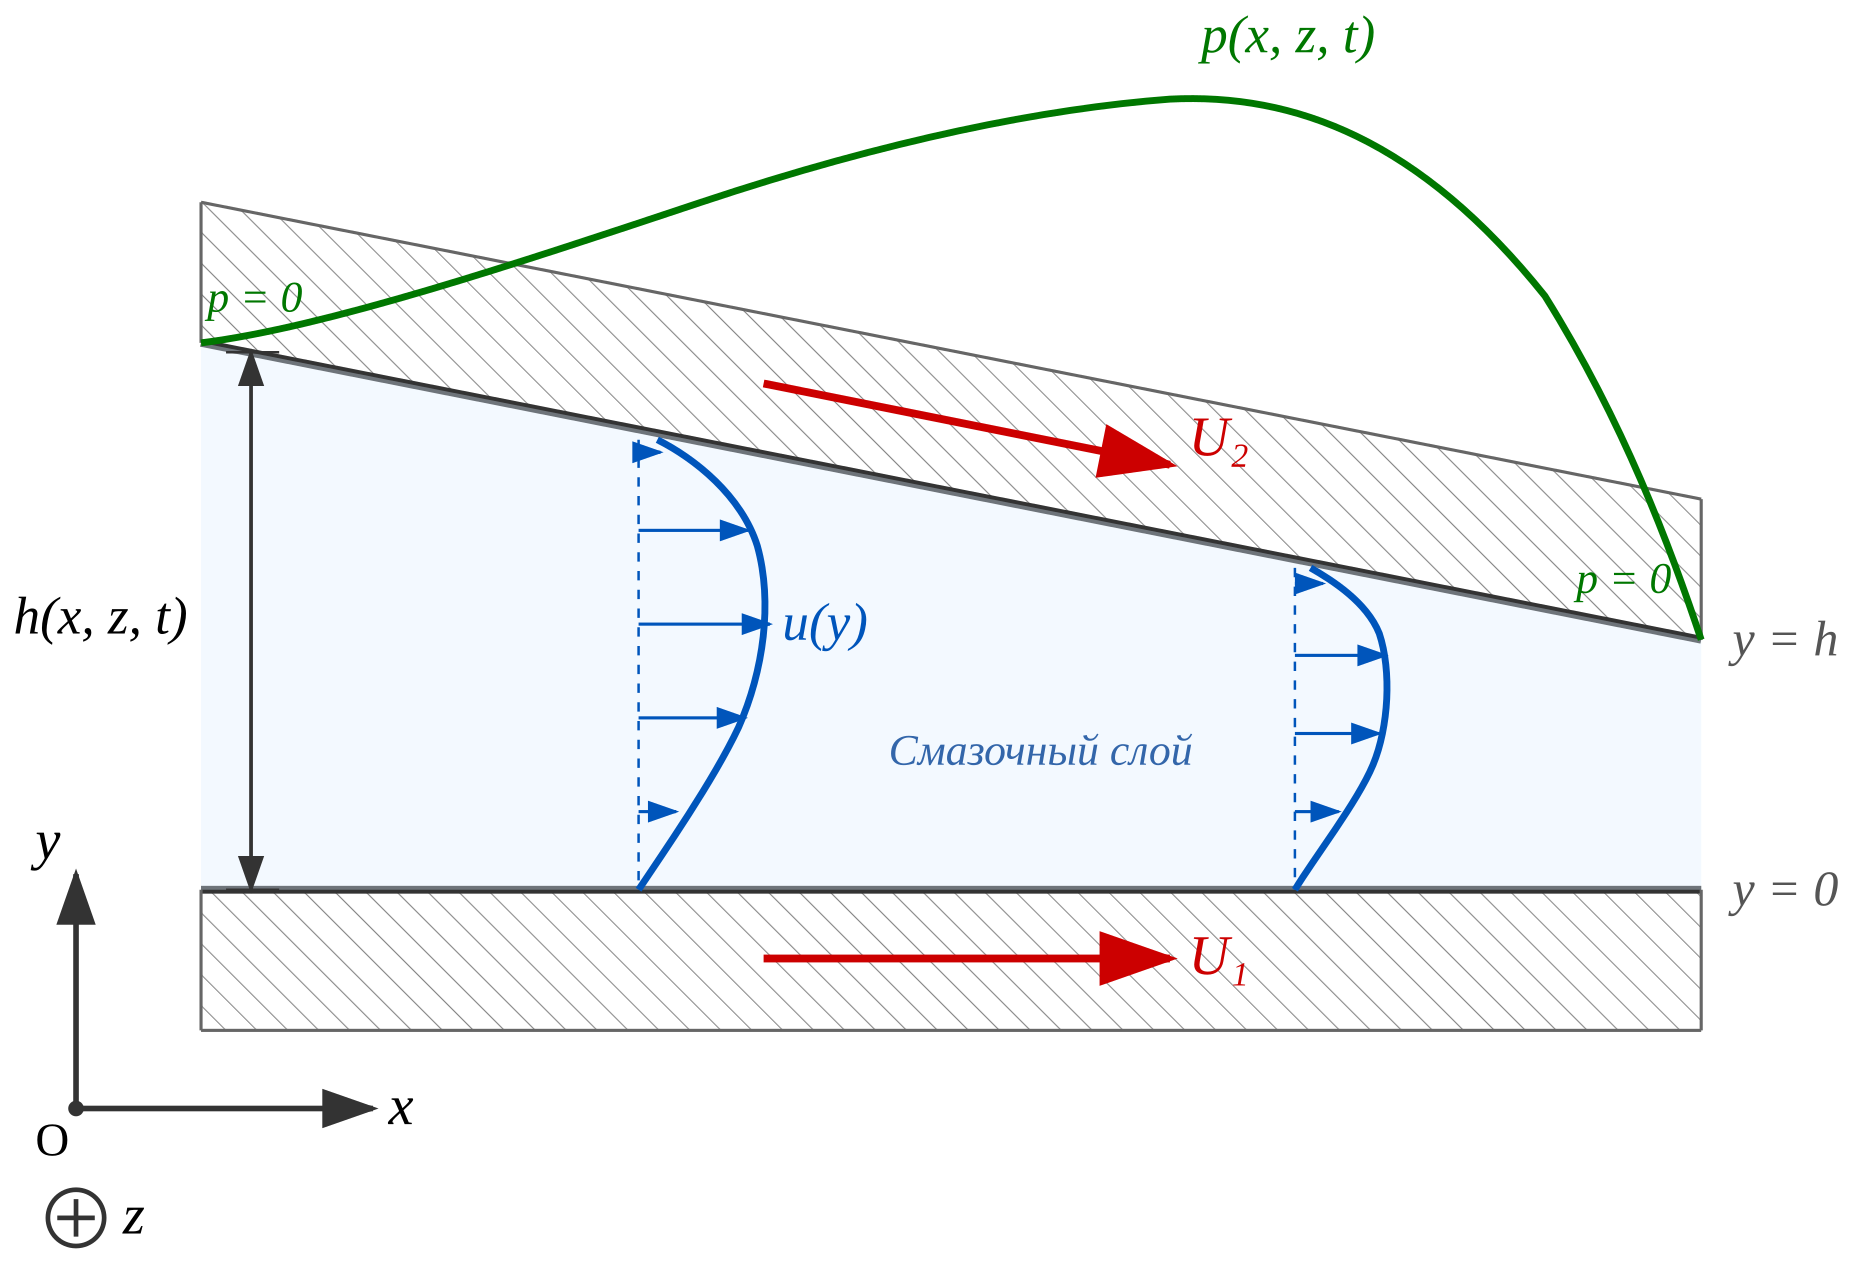
\includegraphics[width=\textwidth,height=0.9\textheight,keepaspectratio]{figures/ch02/fig_2_1.png}
\caption{Схема смазочного слоя между двумя поверхностями}
\label{fig:lubrication_scheme}
\end{figure}

\subsubsection*{Основные допущения}

Вывод уравнения Рейнольдса основан на следующих физических допущениях:

\begin{enumerate}
\item Жидкость ньютоновская: касательные напряжения пропорциональны скоростям деформации, в частности $\tau_{xy} = \mu\,\partial u/\partial y$, $\tau_{yz} = \mu\,\partial w/\partial y$.
\item Жидкость несжимаемая: $\rho = \mathrm{const}$.
\item Тонкий слой: $H \ll L$, где $H$ -- характерный (порядковый) масштаб толщины смазочного слоя $h(x,z,t)$; малые уклоны поверхностей $|\partial h/\partial x| \ll 1$, $|\partial h/\partial z| \ll 1$.
\item Течение ламинарное, инерционные эффекты пренебрежимо малы: $\mathrm{Re}\cdot\epsilon \ll 1$, где $\epsilon = H/L$.
\item Давление постоянно по толщине слоя: $\partial p/\partial y \approx 0$ (следствие смазочной аппроксимации).
\item Динамическая вязкость постоянна: $\mu = \mathrm{const}$ (температурная зависимость рассматривается отдельно при необходимости).
\item На границах жидкости и твёрдых поверхностей выполняется условие прилипания (no-slip).
\item Объёмные силы (гравитация и др.) малы по сравнению с градиентом давления и не учитываются.
\end{enumerate}

\subsubsection*{Исходные уравнения}

Движение жидкости описывается уравнениями Навье--Стокса для несжимаемой жидкости:

\begin{equation}
\rho\left(\frac{\partial \mathbf{v}}{\partial t} + (\mathbf{v} \cdot \nabla)\mathbf{v}\right) = -\nabla p + \mu \nabla^2 \mathbf{v},
\label{eq:navier_stokes}
\end{equation}

и уравнением неразрывности:

\begin{equation}
\nabla \cdot \mathbf{v} = 0,
\label{eq:continuity}
\end{equation}
\begin{conditions}
$\mathbf{v} = (u, v, w)$ -- вектор скорости;\\
$\rho$ -- плотность жидкости;\\
$p$ -- давление;\\
$\mu$ -- динамическая вязкость.
\end{conditions}
В компонентной форме уравнения движения приведены в приложении~А. Уравнение неразрывности~\eqref{eq:continuity} в компонентной записи имеет вид:

\begin{equation}
\frac{\partial u}{\partial x} + \frac{\partial v}{\partial y} + \frac{\partial w}{\partial z} = 0.
\label{eq:continuity_comp}
\end{equation}

Далее, на основе анализа порядков величин, будет получена смазочная аппроксимация и выведено уравнение Рейнольдса.

\subsubsection*{Масштабирование и оценка порядков величин}

Для анализа уравнений введём характерные масштабы задачи:

$L$ -- характерный размер в направлениях $x$ и $z$ (длина подшипника);

$H$ -- характерная толщина смазочного слоя;

$U$ -- характерная скорость движения поверхностей;

$P$ -- характерное давление.

Безразмерные переменные вводятся следующим образом:

\begin{equation}
\bar{x} = \frac{x}{L}, \quad \bar{y} = \frac{y}{H}, \quad \bar{z} = \frac{z}{L}, \quad \bar{u} = \frac{u}{U}, \quad \bar{v} = \frac{v}{V_0}, \quad \bar{w} = \frac{w}{U}, \quad \bar{p} = \frac{p}{P},
\end{equation}
где $V_0$ -- характерная скорость в направлении $y$, которую нужно определить из уравнения неразрывности.

Из уравнения неразрывности следует оценка:

\begin{equation}
\frac{U}{L} \sim \frac{V_0}{H} \quad \Rightarrow \quad V_0 \sim U\frac{H}{L} = U\,\epsilon.
\end{equation}

Ключевым параметром в теории смазки является отношение:

\begin{equation}
\epsilon = \frac{H}{L} \ll 1,
\label{eq:epsilon}
\end{equation}
которое характеризует малость толщины слоя по сравнению с его протяжённостью.

Подставляя безразмерные переменные в компонентные уравнения движения, получаем оценки для различных членов. Из $x$-компоненты уравнения движения при смазочной аппроксимации доминирующий баланс имеет вид:

\begin{equation}
\frac{\partial p}{\partial x} \sim \mu\,\frac{\partial^2 u}{\partial y^2} \quad \Rightarrow \quad \frac{P}{L} \sim \mu\,\frac{U}{H^2} \quad \Rightarrow \quad P \sim \mu\,U\,\frac{L}{H^2}.
\label{eq:pressure_scale}
\end{equation}

Характерное давление определяется балансом вязкого сопротивления потоку в тонком зазоре и продольного градиента давления.

Вводим число Рейнольдса для смазочного слоя:

\begin{equation}
\mathrm{Re} = \frac{\rho U H}{\mu}.
\end{equation}

Отношение инерционных членов к вязким оценивается как:

\begin{equation}
\frac{\rho U^2/L}{P/L} \sim \frac{\rho U^2}{\mu U L/H^2} = \underbrace{\frac{\rho U H}{\mu}}_{\mathrm{Re}}\;\underbrace{\frac{H}{L}}_{\epsilon} = \mathrm{Re}\,\epsilon.
\label{eq:Re_epsilon}
\end{equation}

При условии $\mathrm{Re}\,\epsilon \ll 1$ (что выполняется в большинстве практических случаев) инерционные члены в уравнениях движения пренебрежимо малы по сравнению с вязкими и градиентом давления. Малость этого параметра означает, что инерция жидкости подавлена тонкостью смазочного слоя ($\epsilon = H/L \ll 1$), и течение полностью определяется балансом вязких сил и градиента давления.

Анализируя порядки производных с учётом $\epsilon \ll 1$, получаем:

\begin{equation}
\frac{\partial^2}{\partial y^2} \gg \frac{\partial^2}{\partial x^2}, \quad \frac{\partial^2}{\partial y^2} \gg \frac{\partial^2}{\partial z^2}.
\end{equation}

Таким образом, в $x$- и $z$-компонентах уравнения движения доминируют члены:

\begin{equation}
\frac{\partial p}{\partial x} \sim \mu\frac{\partial^2 u}{\partial y^2}, \quad \frac{\partial p}{\partial z} \sim \mu\frac{\partial^2 w}{\partial y^2}.
\end{equation}

Из $y$-компоненты уравнения движения следует, что величина $\partial p/\partial y$ мала по сравнению с $\partial p/\partial x$ и $\partial p/\partial z$ и имеет порядок $O(\epsilon^2)$, откуда:

\begin{equation}
\frac{\partial p}{\partial y} \approx 0.
\label{eq:dp_dy_zero}
\end{equation}

Это означает, что давление в смазочном слое не зависит от координаты $y$: $p = p(x, z, t)$.

\subsubsection*{Упрощённые уравнения движения}

С учётом сделанных допущений уравнения движения принимают вид:

\begin{equation}
\label{eq:simplified_xz}
\begin{aligned}
\frac{\partial p}{\partial x} &= \mu\frac{\partial^2 u}{\partial y^2}, \\
\frac{\partial p}{\partial z} &= \mu\frac{\partial^2 w}{\partial y^2}.
\end{aligned}
\end{equation}

Уравнение неразрывности сохраняет форму~\eqref{eq:continuity_comp}.

\subsubsection*{Граничные условия}

На поверхностях выполняются условия прилипания (no-slip):

\begin{equation}
\begin{aligned}
&y = 0: \quad u = U_1(x, z, t), \quad w = W_1(x, z, t), \quad v = V_1(x, z, t), \\
&y = h: \quad u = U_2(x, z, t), \quad w = W_2(x, z, t), \quad v = V_2(x, z, t),
\end{aligned}
\label{eq:boundary_conditions}
\end{equation}
где $U_i$, $W_i$, $V_i$ -- компоненты скорости соответствующих поверхностей. В общем случае скорости поверхностей могут зависеть от координат и времени. Далее при выводе уравнения Рейнольдса величины $U_i$ и $W_i$ полагаются постоянными вдоль соответствующей поверхности, что корректно для основных типов подшипников, рассматриваемых в настоящей работе.

\subsubsection*{Профиль скорости}

Интегрируя уравнение~\eqref{eq:simplified_xz} дважды по $y$ и используя граничные условия~\eqref{eq:boundary_conditions}, получаем профиль скорости в направлении $x$:

\begin{equation}
u(x, y, z, t) = U_1 + \frac{y}{h}(U_2 - U_1) + \frac{1}{2\mu}\frac{\partial p}{\partial x}y(y - h).
\label{eq:velocity_profile_u}
\end{equation}

Аналогично для направления $z$:

\begin{equation}
w(x, y, z, t) = W_1 + \frac{y}{h}(W_2 - W_1) + \frac{1}{2\mu}\frac{\partial p}{\partial z}y(y - h).
\label{eq:velocity_profile_w}
\end{equation}

Профиль скорости~\eqref{eq:velocity_profile_u} состоит из двух частей: линейной (куэттовский поток, обусловленный движением поверхностей) и параболической (пуазейлевский поток, обусловленный градиентом давления).

\subsubsection*{Объёмный расход}

Объёмный расход жидкости через единицу длины перпендикулярно направлению $x$ определяется интегрированием скорости по толщине слоя:

\begin{equation}
q_x = \int_0^h u \,\mathrm{d}y.
\end{equation}

Подставляя выражение~\eqref{eq:velocity_profile_u}:

\begin{equation}
q_x = \int_0^h \left[U_1 + \frac{y}{h}(U_2 - U_1) + \frac{1}{2\mu}\frac{\partial p}{\partial x}y(y - h)\right] dy.
\end{equation}

Вычисляем интегралы:

\begin{equation}
\begin{aligned}
&\int_0^h U_1 \,\mathrm{d}y = U_1 h, \\
&\int_0^h \frac{y}{h}(U_2 - U_1) \,\mathrm{d}y = \frac{U_2 - U_1}{h} \cdot \frac{h^2}{2} = \frac{h}{2}(U_2 - U_1), \\
&\int_0^h \frac{1}{2\mu}\frac{\partial p}{\partial x}y(y - h) \,\mathrm{d}y = \frac{1}{2\mu}\frac{\partial p}{\partial x}\left(\frac{h^3}{3} - \frac{h^3}{2}\right) = -\frac{h^3}{12\mu}\frac{\partial p}{\partial x}.
\end{aligned}
\end{equation}

Окончательно для расхода в направлении $x$:

\begin{equation}
q_x = \frac{h}{2}(U_1 + U_2) - \frac{h^3}{12\mu}\frac{\partial p}{\partial x}.
\label{eq:flow_rate_x}
\end{equation}

Аналогично для направления $z$:

\begin{equation}
q_z = \frac{h}{2}(W_1 + W_2) - \frac{h^3}{12\mu}\frac{\partial p}{\partial z}.
\label{eq:flow_rate_z}
\end{equation}

\subsubsection*{Вывод уравнения Рейнольдса}

Из уравнения неразрывности~\eqref{eq:continuity}, интегрируя по толщине слоя от $y = 0$ до $y = h$:

\begin{equation}
\int_0^h \frac{\partial u}{\partial x} \,\mathrm{d}y + \int_0^h \frac{\partial v}{\partial y} \,\mathrm{d}y + \int_0^h \frac{\partial w}{\partial z} \,\mathrm{d}y = 0.
\end{equation}

Используя правило Лейбница для дифференцирования интеграла:

\begin{equation}
\frac{\partial}{\partial x}\int_0^h u \,\mathrm{d}y = \int_0^h \frac{\partial u}{\partial x} \,\mathrm{d}y + u|_{y=h}\frac{\partial h}{\partial x},
\end{equation}
и аналогично для $z$. Таким образом, интегралы производных в уравнении неразрывности выражаются как:

\begin{equation}
\label{eq:leibniz_applied}
\begin{split}
&\int_0^h \frac{\partial u}{\partial x}\,\mathrm{d}y = \frac{\partial}{\partial x}\!\int_0^h u\,\mathrm{d}y
  - u\big|_{y=h}\,\frac{\partial h}{\partial x}, \\
&\int_0^h \frac{\partial w}{\partial z}\,\mathrm{d}y = \frac{\partial}{\partial z}\!\int_0^h w\,\mathrm{d}y
  - w\big|_{y=h}\,\frac{\partial h}{\partial z}.
\end{split}
\end{equation}

Для второго интеграла:

\begin{equation}
\int_0^h \frac{\partial v}{\partial y} \,\mathrm{d}y = v|_{y=h} - v|_{y=0} = V_2 - V_1.
\end{equation}

Кинематическое условие на верхней поверхности $y = h(x,z,t)$:

\begin{equation}
V_2 = \frac{\partial h}{\partial t} + U_2\frac{\partial h}{\partial x} + W_2\frac{\partial h}{\partial z}.
\label{eq:kinematic_upper}
\end{equation}

Нижняя поверхность полагается плоской и неподвижной в направлении $y$, откуда $V_1 = 0$. Здесь использовано условие прилипания на верхней поверхности: $u(h) = U_2$, $w(h) = W_2$, $v(h) = V_2$. Подставляя~\eqref{eq:leibniz_applied} и кинематическое условие~\eqref{eq:kinematic_upper} в интегрированное уравнение неразрывности, после сокращения членов $U_2\,\partial h/\partial x$ и $W_2\,\partial h/\partial z$, приходим к уравнению:

Используя определения расходов~\eqref{eq:flow_rate_x} и~\eqref{eq:flow_rate_z}:

\begin{equation}
\frac{\partial q_x}{\partial x} + \frac{\partial q_z}{\partial z} + \frac{\partial h}{\partial t} = 0.
\label{eq:continuity_integrated}
\end{equation}

Уравнение~\eqref{eq:continuity_integrated} допускает наглядную интерпретацию в терминах контрольного объёма (рисунок~\ref{fig:control_volume}): изменение толщины слоя $\partial h/\partial t$ компенсируется потоками $q_x$ и $q_z$ через боковые грани элемента $dx \times dz$.

% [РИСУНОК: Контрольный объём смазочного слоя]
% Должен показывать:
% - Элемент dx × dz, толщина h
% - Потоки q_x и q_x + ∂q_x/∂x·dx через левую и правую грани
% - Потоки q_z и q_z + ∂q_z/∂z·dz через переднюю и заднюю грани
% - Стрелка ∂h/∂t сверху (выжимание)
% - Формула баланса: ∂q_x/∂x + ∂q_z/∂z + ∂h/∂t = 0
\begin{figure}[!ht]
\centering
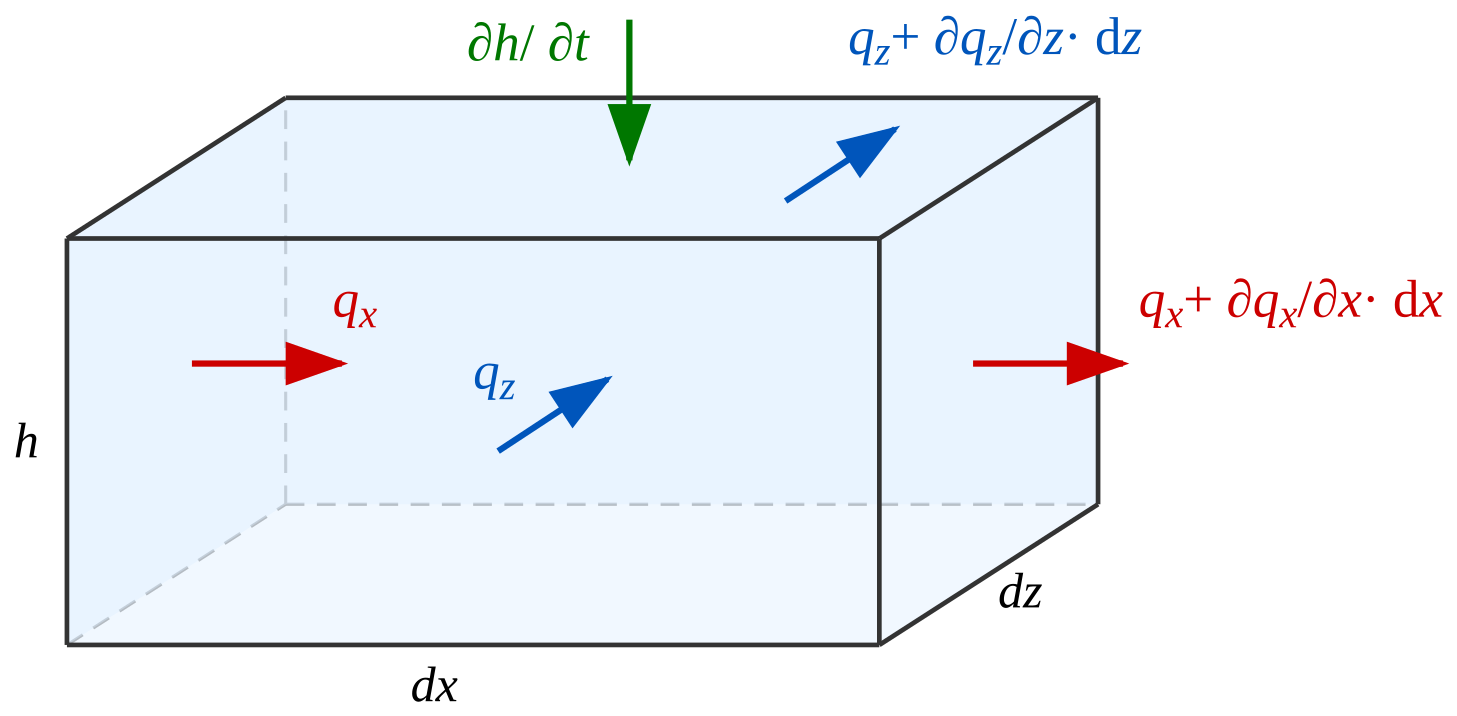
\includegraphics[width=\textwidth,height=0.9\textheight,keepaspectratio]{figures/ch02/fig_2_2.png}
\caption{Контрольный объём смазочного слоя и баланс расходов}
\label{fig:control_volume}
\end{figure}

\FloatBarrier

Подставляя выражения для $q_x$ и $q_z$:

\begin{equation}
\begin{split}
&\frac{\partial}{\partial x}\left[\frac{h}{2}(U_1 + U_2) - \frac{h^3}{12\mu}\frac{\partial p}{\partial x}\right] + {} \\
&+ \frac{\partial}{\partial z}\left[\frac{h}{2}(W_1 + W_2) - \frac{h^3}{12\mu}\frac{\partial p}{\partial z}\right] + \frac{\partial h}{\partial t} = 0.
\end{split}
\end{equation}

Раскрывая производные:

\begin{equation}
\label{eq:reynolds_full}
\begin{split}
&\frac{\partial}{\partial x}\left(\frac{h^3}{12\mu}\frac{\partial p}{\partial x}\right) + \frac{\partial}{\partial z}\left(\frac{h^3}{12\mu}\frac{\partial p}{\partial z}\right) = {} \\
&= \frac{\partial}{\partial x}\left[\frac{h}{2}(U_1 + U_2)\right] + \frac{\partial}{\partial z}\left[\frac{h}{2}(W_1 + W_2)\right] + \frac{\partial h}{\partial t}.
\end{split}
\end{equation}

Уравнение~\eqref{eq:reynolds_full} является \textbf{обобщённым уравнением Рейнольдса} для случая нестационарного течения с подвижными границами произвольной формы.
Вязкость~$\mu$ записана под знаком производных, что обеспечивает корректность формулы и при переменной вязкости $\mu = \mu(x, z)$ (например, при учёте температурной зависимости в главе~4).

Для стационарного случая ($\partial h/\partial t = 0$) и при условии $W_1 = W_2 = 0$ (движение только в направлении $x$) уравнение упрощается:

\begin{equation}
\frac{\partial}{\partial x}\left(\frac{h^3}{12\mu}\frac{\partial p}{\partial x}\right) + \frac{\partial}{\partial z}\left(\frac{h^3}{12\mu}\frac{\partial p}{\partial z}\right) = \frac{U_1 + U_2}{2}\frac{\partial h}{\partial x}.
\label{eq:reynolds_steady}
\end{equation}

Уравнение~\eqref{eq:reynolds_steady} представляет собой \textbf{классическое уравнение Рейнольдса} для гидродинамической смазки.

В случае одной движущейся поверхности (например, $U_1 = U$, $U_2 = 0$) и постоянной вязкости $\mu = \mathrm{const}$ обе части уравнения можно умножить на~$12\mu$, что даёт эквивалентную форму, удобную для численной реализации:

\begin{equation}
\frac{\partial}{\partial x}\left(h^3\frac{\partial p}{\partial x}\right) + \frac{\partial}{\partial z}\left(h^3\frac{\partial p}{\partial z}\right) = 6\mu\,U\frac{\partial h}{\partial x}.
\label{eq:reynolds_one_surface}
\end{equation}

Полученное уравнение Рейнольдса~\eqref{eq:reynolds_one_surface} является основным уравнением теории гидродинамической смазки и связывает распределение давления $p(x, z)$ в смазочном слое с геометрией зазора $h(x, z)$ и скоростью движения поверхности $U$~\cite{hori2002,szeri1998}.

Следует отметить, что при решении уравнения Рейнольдса в областях расходящегося зазора могут возникать зоны отрицательного давления, не имеющие физического смысла. Для корректного описания таких областей необходима массо-сохраняющая модель кавитации, которая рассматривается в разделе~2.3 на основе подхода Jakobsson--Floberg--Olsson (JFO).

\FloatBarrier
\subsection{Постановка задачи для торцевого зазора}

% Упорный подшипник (thrust bearing)
% Полная постановка задачи: геометрия, кинематика, уравнение Рейнольдса,
% граничные условия, расходы, целевые функционалы

Рассмотрим упорный (осевой) подшипник скольжения -- узел, в котором осевая нагрузка воспринимается тонким слоем вязкой жидкости, заключённым между двумя поверхностями: вращающимся диском (ротором) и неподвижной опорной поверхностью (колодкой, или сектором). Несущая способность подшипника обусловлена гидродинамическим давлением, которое генерируется в сходящемся зазоре при относительном движении поверхностей.

Упорные подшипники скольжения находят широкое применение в инженерной практике. В турбинах гидро- и теплоэнергетических установок они воспринимают осевое усилие, создаваемое рабочим телом на рабочем колесе. В центробежных насосах и компрессорах упорные подшипники фиксируют осевое положение ротора, предотвращая контакт вращающихся и неподвижных элементов. В тяжёлых прокатных станах и вертикальных гидрогенераторах упорные подшипники несут вес ротора и всего рабочего оборудования~\cite{hori2002,szeri1998}.

Цель постановки: для заданной геометрии зазора $h(r,\theta)$ и режима движения поверхностей получить распределение давления $p(r,\theta)$ в смазочном слое. По найденному полю давления далее вычисляются интегральные характеристики, приведённые в подразделе~2.1.7. Все допущения, принятые при выводе уравнения Рейнольдса в подразделе~2.1.1, сохраняют силу: жидкость ньютоновская и несжимаемая, течение ламинарное и стационарное, давление постоянно по толщине смазочного слоя. Далее рассматривается один сектор (колодка) подшипника; полный подшипник состоит из $N$ одинаковых секторов, расположенных равномерно по окружности.


\subsubsection*{Геометрия и система координат}

Для описания упорного подшипника естественно использовать цилиндрические координаты $(r, \theta, y)$:
\begin{itemize}
\item $r$ -- радиальная координата в плоскости подшипника;
\item $\theta$ -- окружная координата, отсчитываемая по направлению вращения;
\item $y$ -- координата по толщине смазочного слоя, направленная перпендикулярно рабочим поверхностям (от $y = 0$ на неподвижной колодке до $y = h$ на вращающемся диске).
\end{itemize}

Область расчёта для одного сектора определяется следующим образом:
\begin{equation}
r \in [R_{\mathrm{in}},\; R_{\mathrm{out}}], \quad \theta \in [\theta_0,\; \theta_1],
\label{eq:thrust_domain}
\end{equation}
\begin{conditions}
$R_{\mathrm{in}}$ и $R_{\mathrm{out}}$ -- внутренний и наружный радиусы рабочей зоны подшипника;\\
$\theta_0$ и $\theta_1$ -- угловые границы сектора.
\end{conditions}
Угловая протяжённость сектора обозначается
\begin{equation}
\beta = \theta_1 - \theta_0.
\label{eq:thrust_beta}
\end{equation}

Граница $\theta_0$ соответствует входной кромке (leading edge), а $\theta_1$ -- выходной кромке (trailing edge) по направлению вращения диска. Толщина смазочного слоя в каждой точке расчётной области составляет $y \in [0,\; h(r,\theta)]$.

Для подшипника из $N$ одинаковых секторов, расположенных равномерно по окружности, угловая протяжённость одного сектора определяется как $\beta = 2\pi/N$ за вычетом углового зазора между соседними колодками. Расчётная область одного сектора схематически изображена на рисунке~\ref{fig:thrust_bearing}.

% [РИСУНОК: Схема упорного подшипника — вид сверху на сектор]
% Должен показывать:
% - Вид сверху на один сектор подшипника
% - Оси r, θ, направление вращения ω
% - Границы R_in, R_out, θ_0, θ_1
% - Угловую протяжённость β
\begin{figure}[!ht]
\centering
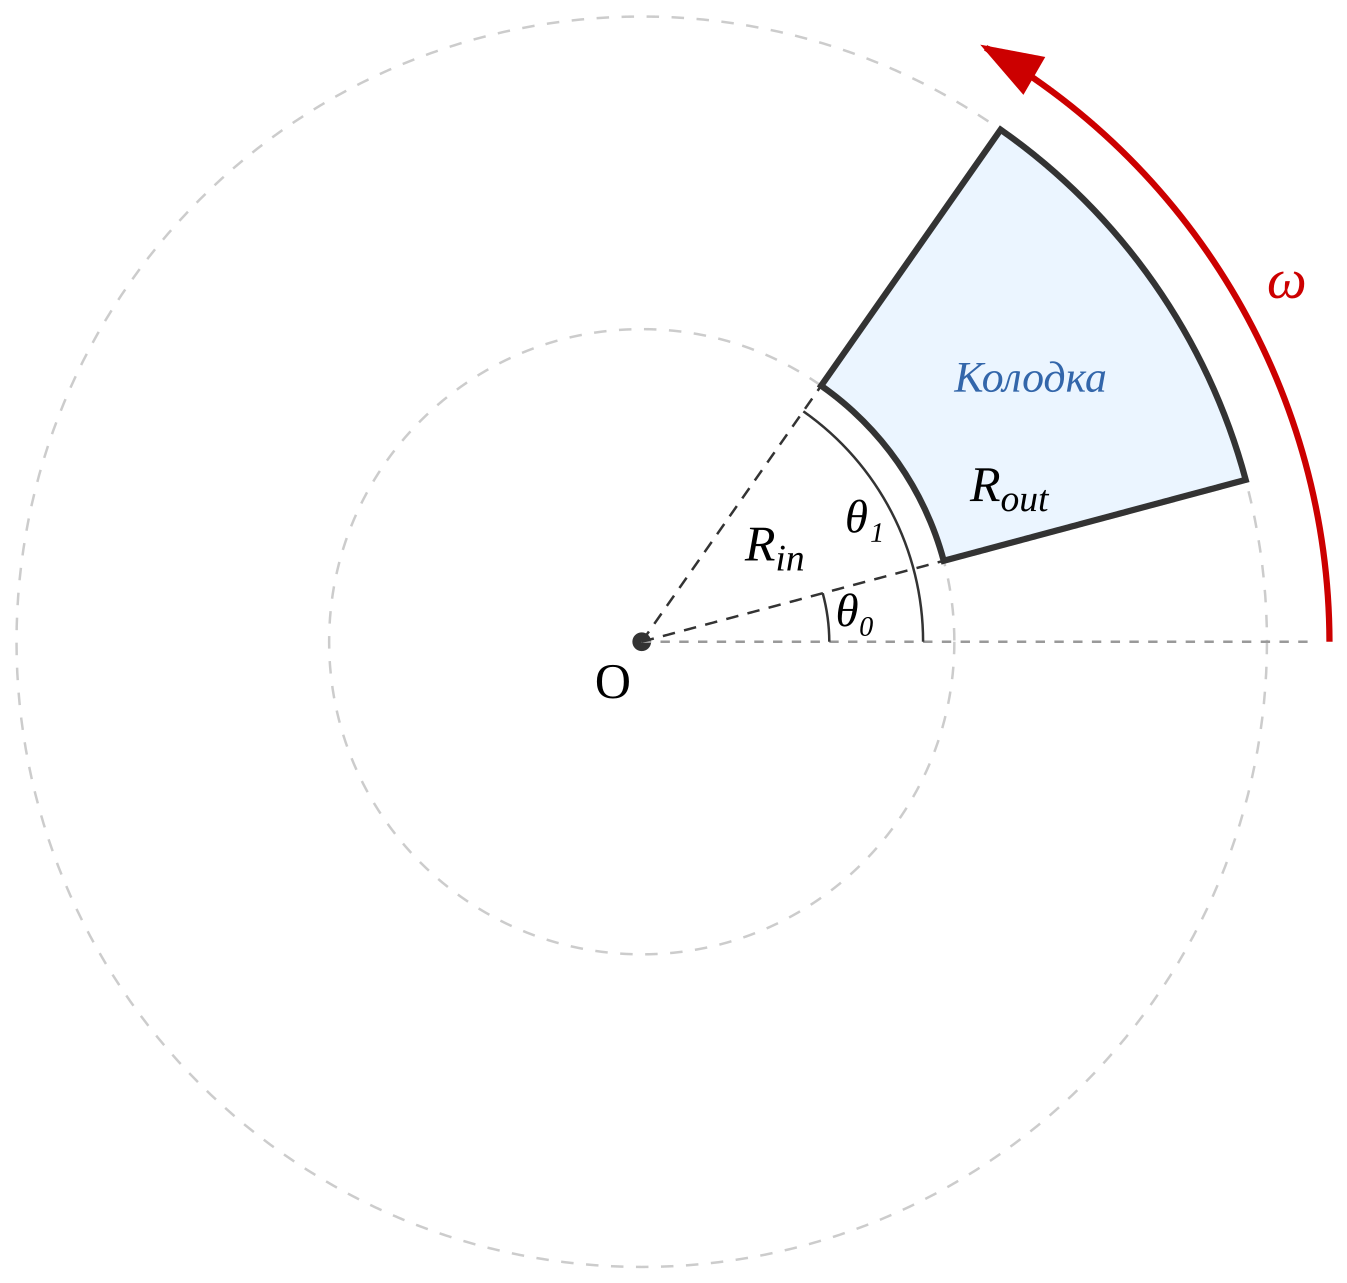
\includegraphics[width=\textwidth,height=0.9\textheight,keepaspectratio]{figures/ch02/fig_2_3.png}
\caption{Схема упорного подшипника: вид сверху на один сектор}
\label{fig:thrust_bearing}
\end{figure}


\subsubsection*{Кинематика движения поверхностей}

Нижняя поверхность ($y = 0$) представляет собой неподвижную колодку, верхняя поверхность ($y = h$) -- вращающийся диск с постоянной угловой скоростью $\omega$. Тангенциальная (окружная) скорость скольжения вращающегося диска в точке с радиальной координатой $r$ составляет:
\begin{equation}
U_\theta(r) = \omega\,r.
\label{eq:thrust_U_theta}
\end{equation}

Радиальные скорости обеих поверхностей равны нулю: $U_{r,1} = U_{r,2} = 0$. В стационарном режиме нормальные скорости поверхностей также обращаются в нуль: $V_1 = V_2 = 0$, что исключает эффект выжимания ($\partial h/\partial t = 0$).

Динамическая вязкость смазки полагается постоянной: $\mu = \mathrm{const}$ (допущение~6 из подраздела~2.1.1). Влияние температурной зависимости вязкости $\mu(T)$ на характеристики подшипника рассматривается отдельно в главе~4.

Вращение диска создаёт тангенциальный увлекающий поток (куэттовскую составляющую течения): жидкость, увлекаемая подвижной поверхностью за счёт условия прилипания, движется в окружном направлении. Когда такой поток проходит через участок зазора с уменьшающейся толщиной, условие неразрывности (сохранения массы) приводит к росту давления в смазочном слое -- именно этот механизм, называемый клиновым эффектом, обеспечивает несущую способность подшипника.


\subsubsection*{Закон толщины смазочного слоя}

В общем случае толщина смазочного слоя является заданной функцией координат:
\begin{equation}
h = h(r, \theta),
\label{eq:thrust_h_general}
\end{equation}
определяющей профиль зазора между колодкой и вращающимся диском. В разделе~2.2 функция $h(r,\theta)$ будет расширена для учёта детерминированных микроструктур рабочей поверхности.

Для тестирования численных методов и верификации результатов широко используется базовая геометрия -- линейный клин, в котором толщина зазора линейно изменяется по окружной координате:
\begin{equation}
h(r,\theta) = h_{\mathrm{in}} + (h_{\mathrm{out}} - h_{\mathrm{in}})\,\frac{\theta - \theta_0}{\theta_1 - \theta_0},
\label{eq:thrust_h_wedge}
\end{equation}
\begin{conditions}
$h_{\mathrm{in}} = h(\theta_0)$ -- толщина смазочного слоя на входной кромке сектора;\\
$h_{\mathrm{out}} = h(\theta_1)$ -- толщина на выходной кромке.
\end{conditions}
Необходимым условием генерации давления является сходящийся характер зазора по направлению движения, т.\,е.
\begin{equation}
h_{\mathrm{in}} > h_{\mathrm{out}}.
\label{eq:thrust_convergence_condition}
\end{equation}

В частном случае $h_{\mathrm{in}} = h_{\mathrm{out}}$ (плоскопараллельный зазор) правая часть уравнения Рейнольдса обращается в нуль и давление не генерируется.

В формуле~\eqref{eq:thrust_h_wedge} величины $h_{\mathrm{in}}$ и $h_{\mathrm{out}}$ приняты постоянными по радиальной координате $r$, что соответствует плоскому клину. Минимальная толщина смазочного слоя обозначается
\begin{equation}
h_{\min} = \min_{(r,\theta)} h(r,\theta);
\label{eq:thrust_h_min}
\end{equation}
для линейного клина $h_{\min} = h_{\mathrm{out}}$.

Для характеристики формы клина вводятся безразмерные параметры конвергенции:
\begin{equation}
K = \frac{h_{\mathrm{in}}}{h_{\mathrm{out}}}, \quad \delta = \frac{h_{\mathrm{in}} - h_{\mathrm{out}}}{h_{\mathrm{out}}} = K - 1.
\label{eq:thrust_convergence}
\end{equation}

При $K = 1$ ($\delta = 0$) зазор является плоскопараллельным и давление не генерируется. Оптимальное значение параметра $K$, обеспечивающее максимальную несущую способность, зависит от соотношения размеров подшипника и определяется численно.

Помимо линейного клина, на практике применяются более сложные профили зазора: ступенчатый (профиль Рэлея), параболический, составной (с плоским участком и клиновой частью). Все перечисленные варианты описываются тем же уравнением Рейнольдса при соответствующем задании функции $h(r,\theta)$. Линейный клин~\eqref{eq:thrust_h_wedge} используется в настоящей работе как базовый верификационный профиль; в реальной колодке профиль зазора $h(r,\theta)$ определяется наклоном опоры и формой рабочей поверхности, что может приводить к зависимости $h$ от радиальной координаты~$r$. Продольное сечение клинового зазора при фиксированном $r$ аналогично общей схеме смазочного слоя (рисунок~\ref{fig:lubrication_scheme}), где горизонтальная координата~$x$ заменяется на~$\theta$, нижняя поверхность соответствует неподвижной колодке, а верхняя~-- плоскому вращающемуся диску со скоростью~$U_\theta = \omega r$. Зазор сужается от~$h_{\mathrm{in}}$ на входном крае колодки до~$h_{\mathrm{out}}$ на выходном.



\subsubsection*{Уравнение Рейнольдса в цилиндрических координатах}

Обобщённое уравнение Рейнольдса~\eqref{eq:reynolds_full}, полученное в подразделе~2.1.1 в декартовых координатах, необходимо переписать в цилиндрических координатах $(r, \theta)$, естественных для задачи об упорном подшипнике. Переход осуществляется введением дуговой координаты $s = r\theta$, вдоль которой производная принимает вид $\partial/\partial s = (1/r)\,\partial/\partial\theta$. Оператор дивергенции и градиента в плоскости $(r, \theta)$ приобретает стандартные множители $1/r$ и $1/r^2$, присутствующие в левой части уравнения Рейнольдса.

В рассматриваемой задаче скорость скольжения направлена по окружной координате~$\theta$: нижняя поверхность неподвижна ($U_{\theta,1} = 0$), верхняя движется со скоростью $U_{\theta,2} = \omega r$; радиальные скорости обеих поверхностей равны нулю. Правая часть обобщённого уравнения Рейнольдса~\eqref{eq:reynolds_full} в цилиндрических координатах записывается в дивергентной форме:
\begin{equation}
\mathrm{RHS} = \frac{1}{r}\frac{\partial}{\partial\theta}\!\left[\frac{h}{2}
(U_{\theta,1} + U_{\theta,2})\right], \quad U_{\theta,1} = 0,\quad U_{\theta,2} = \omega r,
\label{eq:thrust_rhs_div}
\end{equation}
откуда, учитывая, что произведение $\omega r$ не зависит от~$\theta$:
\begin{equation}
\frac{U_{\theta,1} + U_{\theta,2}}{2}\,\frac{1}{r}\,\frac{\partial h}{\partial \theta} = \frac{\omega r}{2}\,\frac{1}{r}\,\frac{\partial h}{\partial \theta} = \frac{\omega}{2}\,\frac{\partial h}{\partial \theta}.
\label{eq:thrust_rhs_derivation}
\end{equation}

Стационарное уравнение Рейнольдса для несжимаемой ньютоновской жидкости в цилиндрических координатах принимает вид:
\begin{equation}
\label{eq:thrust_reynolds}
\frac{1}{r}\frac{\partial}{\partial r}\!\left[r\,\frac{h^3}{12\mu}\,\frac{\partial p}{\partial r}\right] + \frac{1}{r^2}\frac{\partial}{\partial \theta}\!\left[\frac{h^3}{12\mu}\,\frac{\partial p}{\partial \theta}\right] = \frac{\omega}{2}\,\frac{\partial h}{\partial \theta}.
\end{equation}

Множители $1/r$ и $1/r^2$ перед производными в левой части обусловлены дивергентной формой эллиптического оператора $\nabla \cdot (h^3 \nabla p)$ в цилиндрических координатах. Оператор Лапласа является его частным случаем при $h = \mathrm{const}$.

Умножая обе части уравнения~\eqref{eq:thrust_reynolds} на~$12\mu$ (что допустимо при $\mu = \mathrm{const}$), получаем эквивалентную форму, удобную для численной реализации:
\begin{equation}
\frac{1}{r}\frac{\partial}{\partial r}\!\left[r\,h^3\,\frac{\partial p}{\partial r}\right] + \frac{1}{r^2}\frac{\partial}{\partial \theta}\!\left[h^3\,\frac{\partial p}{\partial \theta}\right] = 6\mu\omega\,\frac{\partial h}{\partial \theta}.
\label{eq:thrust_reynolds_num}
\end{equation}

Уравнение~\eqref{eq:thrust_reynolds_num} является основным расчётным уравнением для упорного подшипника в настоящей работе.

Левая часть уравнений~\eqref{eq:thrust_reynolds}-\eqref{eq:thrust_reynolds_num} представляет собой эллиптический оператор, описывающий перераспределение давления через вязкий смазочный слой: давление <<диффундирует>> как в радиальном, так и в окружном направлениях, причём <<проводимость>> пропорциональна кубу толщины зазора~$h^3$. Правая часть -- источниковый член, обусловленный изменением толщины зазора в направлении движения (клиновой эффект). При $\partial h/\partial \theta = 0$ (плоскопараллельный зазор) правая часть обращается в нуль, и при однородных граничных условиях уравнение допускает лишь тривиальное решение $p = 0$ -- давление не генерируется.

При наличии детерминированных микроструктур на рабочей поверхности функция $h(r,\theta)$ приобретает быстрые локальные вариации. Формально уравнение~\eqref{eq:thrust_reynolds_num} остаётся тем же, однако функция зазора существенно усложняется, что описывается в разделе~2.2.


\subsubsection*{Граничные условия}

Для замыкания уравнения Рейнольдса~\eqref{eq:thrust_reynolds_num} необходимо задать граничные условия на давление по всему контуру расчётной области~\eqref{eq:thrust_domain}. Рассмотрим три практически важных варианта.

\textit{Базовый вариант (атмосферные кромки).} На всех четырёх границах сектора давление принимается равным атмосферному:
\begin{equation}
\begin{aligned}
&p(r,\,\theta_0) = 0, \quad p(r,\,\theta_1) = 0, \\
&p(R_{\mathrm{in}},\,\theta) = 0, \quad p(R_{\mathrm{out}},\,\theta) = 0.
\end{aligned}
\label{eq:thrust_bc_base}
\end{equation}

Здесь давление отсчитывается от атмосферного ($p = p_{\mathrm{abs}} - p_{\mathrm{atm}}$). Условие~\eqref{eq:thrust_bc_base} соответствует изолированному сектору, кромки которого свободно сообщаются с окружающей средой, а принудительная подача смазки отсутствует. Данный вариант является наиболее распространённым при расчёте несамоустанавливающихся колодок.

\textit{Вариант с давлением подачи.} Если система смазки обеспечивает принудительную подачу жидкости через входную кромку сектора, граничное условие на $\theta = \theta_0$ модифицируется:
\begin{equation}
p(r,\,\theta_0) = p_{\mathrm{sup}}(r),
\label{eq:thrust_bc_supply}
\end{equation}
где $p_{\mathrm{sup}}(r)$ -- заданное давление подачи смазки; в простейшем случае $p_{\mathrm{sup}} = \mathrm{const}$. Остальные граничные условия остаются такими же, как в базовом варианте~\eqref{eq:thrust_bc_base}. Величина $p_{\mathrm{sup}}$ определяется конструкцией системы смазки и режимом работы насоса подачи.

\textit{Кавитация.} При решении уравнения Рейнольдса в областях расходящегося зазора расчётное давление может оказаться отрицательным. Отрицательное давление физически не реализуется: при снижении давления ниже давления насыщенных паров смазки жидкость разрывается и образуется кавитационная зона с парогазовой смесью. В простейшей постановке применяют ограничение $p \geq 0$ (условие Гюмбеля), при котором отрицательные давления обнуляются после решения. Такой подход, однако, нарушает закон сохранения массы на границе кавитационной зоны. Корректная массо-сохраняющая постановка, основанная на модели Jakobsson--Floberg--Olsson (JFO), вводится в разделе~2.3. Граница между зоной полного смазочного слоя и кавитационной зоной заранее неизвестна и определяется в процессе решения как часть задачи.

Следует отметить, что условия Дирихле $p = 0$ на всех четырёх границах сектора представляют лишь один из возможных вариантов замыкания задачи. В зависимости от конструкции узла и схемы смазки могут применяться и другие постановки: периодичность по $\theta$ (при моделировании полного кольцевого сегмента без разрывов), условие непротекания через радиальные границы $q_r = 0$, что эквивалентно $\partial p/\partial r = 0$ (при наличии уплотнений или перемычек), а также смешанные условия при комбинированной подаче смазки. Конкретный набор граничных условий определяется конструкцией узла и схемой подвода смазки.

Перечисленные варианты граничных условий схематически показаны на рисунке~\ref{fig:thrust_bc_schemes}.

% [РИСУНОК: Варианты граничных условий на секторе]
% Должен показывать три подрисунка (a), (b), (c):
% (a) Базовый: p = 0 на всех 4 границах сектора
% (b) С подпиткой: p = p_sup на θ = θ_0, остальные p = 0
% (c) Альтернативный: ∂p/∂r = 0 на радиальных границах (уплотнения)
%     или периодичность по θ
% На каждом подрисунке — контур сектора с обозначением ГУ на каждой стороне
\begin{figure}[!ht]
\centering
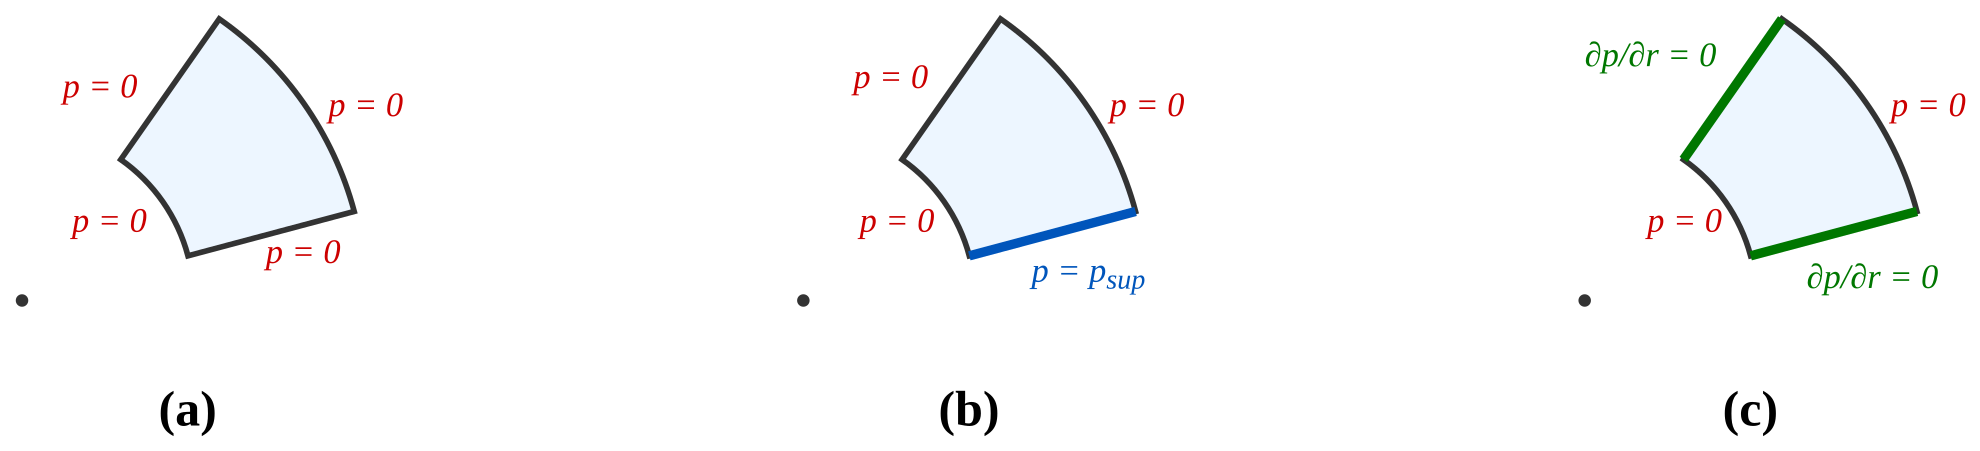
\includegraphics[width=\textwidth,height=0.9\textheight,keepaspectratio]{figures/ch02/fig_2_4.png}
\caption{Варианты граничных условий для упорного подшипника: (a)~$p=0$ на всех четырёх границах сектора (атмосферные кромки); (b)~$p=p_{\mathrm{sup}}$ на входной кромке $\theta=\theta_0$ (принудительная подача), остальные границы $p=0$; (c)~$\partial p/\partial r=0$ на радиальных границах (уплотнения), $p=0$ на дуговых кромках}
\label{fig:thrust_bc_schemes}
\end{figure}

\begin{figure}[!ht]
\centering
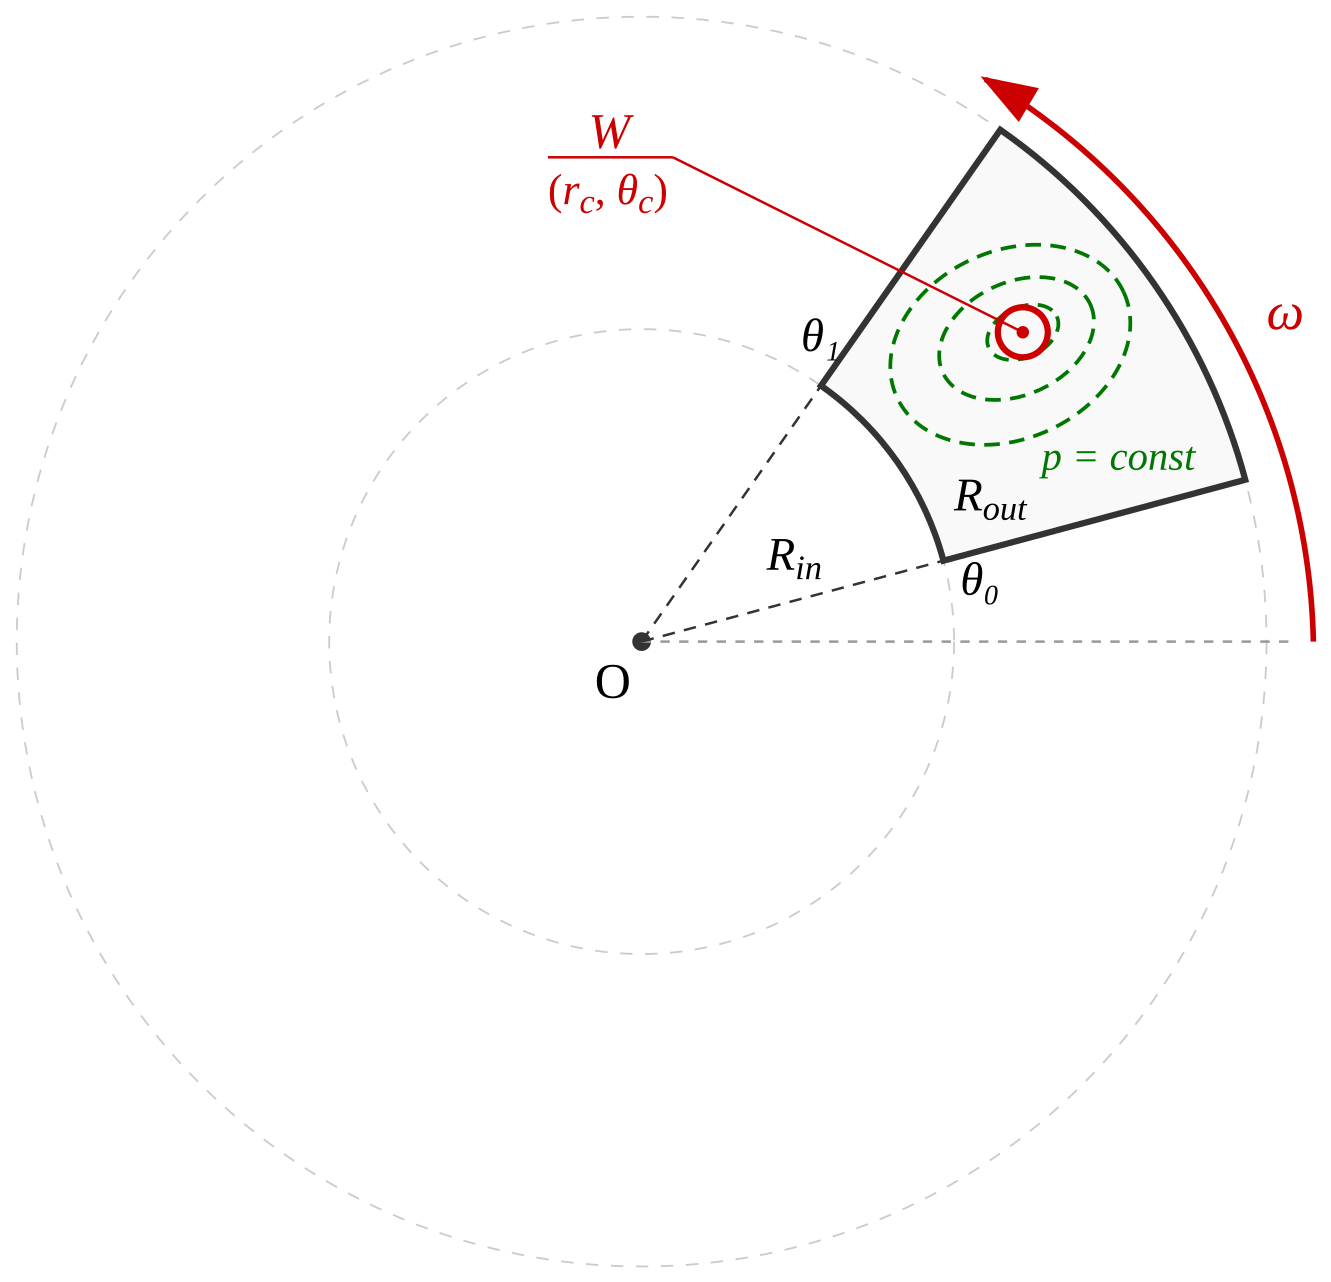
\includegraphics[width=\textwidth,height=0.9\textheight,keepaspectratio]{figures/ch02/fig_2_5.png}
\caption{Результирующая сила~$W$ и изобары давления на секторе упорного подшипника;
  $(r_c,\,\theta_c)$~--- координаты центра давления}
\label{fig:thrust_pressure_map}
\end{figure}


\subsubsection*{Объёмные расходы}

Объёмные расходы жидкости через единицу длины определяются путём интегрирования профилей скорости по толщине смазочного слоя, аналогично выражениям~\eqref{eq:flow_rate_x}-\eqref{eq:flow_rate_z}, полученным в подразделе~2.1.1 в декартовых координатах. Ниже приведены формулы, адаптированные к цилиндрической системе координат.

Радиальный расход (на единицу длины по окружной координате):
\begin{equation}
q_r(r,\theta) = -\frac{h^3}{12\mu}\,\frac{\partial p}{\partial r}.
\label{eq:thrust_q_r}
\end{equation}

Поскольку радиальные скорости обеих поверхностей равны нулю, куэттовская составляющая в радиальном направлении отсутствует. Радиальный расход полностью определяется градиентом давления (пуазейлевская составляющая).

Окружной расход (на единицу длины по радиальной координате):
\begin{equation}
q_\theta(r,\theta) = \frac{h\,\omega\,r}{2} - \frac{h^3}{12\mu\,r}\,\frac{\partial p}{\partial \theta}.
\label{eq:thrust_q_theta}
\end{equation}

Первое слагаемое в~\eqref{eq:thrust_q_theta} представляет куэттовскую составляющую расхода, обусловленную увлечением жидкости вращающейся поверхностью. При $U_{\theta,1}=0$ и $U_{\theta,2}=\omega r$ средняя скорость потока составляет $\bar{U}_\theta = \omega r / 2$, а объёмный расход через единицу длины равен $h\,\bar{U}_\theta = h\omega r/2$. Второе слагаемое -- пуазейлевская составляющая; множитель $1/r$ в знаменателе возникает из-за метрического коэффициента при переходе от производной по дуге $\partial/\partial(r\theta)$ к производной по углу $\partial/\partial\theta$.

Суммарные объёмные расходы через радиальные границы подшипника получаются интегрированием удельных расходов по окружной кромке:
\begin{equation}
\label{eq:thrust_Q_radial}
\begin{split}
&Q_{\mathrm{out}} = \int_{\theta_0}^{\theta_1} q_r(R_{\mathrm{out}}, \theta)\,R_{\mathrm{out}}\,\mathrm{d}\theta, \\
&Q_{\mathrm{in}} = \int_{\theta_0}^{\theta_1} q_r(R_{\mathrm{in}}, \theta)\,R_{\mathrm{in}}\,\mathrm{d}\theta.
\end{split}
\end{equation}

Множитель $R_{\mathrm{out}}$ (соответственно, $R_{\mathrm{in}}$) перед $d\theta$ обусловлен элементом длины дуги $dl = r\,\mathrm{d}\theta$ на окружности радиуса $r$.

Разность $Q_{\mathrm{out}} - Q_{\mathrm{in}}$ определяет утечку смазки через радиальные кромки сектора. Суммарный окружной расход через входную и выходную окружные кромки дополняет баланс массы: полный расход жидкости, поступающей в сектор, равен полному расходу, покидающему его.

Баланс массы в стационарном режиме без выжимания записывается в дифференциальной форме:
\begin{equation}
\frac{1}{r}\,\frac{\partial (r\,q_r)}{\partial r} + \frac{1}{r}\,\frac{\partial q_\theta}{\partial \theta} = 0.
\label{eq:thrust_mass_balance}
\end{equation}

Подстановка выражений~\eqref{eq:thrust_q_r} и~\eqref{eq:thrust_q_theta} в уравнение~\eqref{eq:thrust_mass_balance} приводит к уравнению Рейнольдса~\eqref{eq:thrust_reynolds}, что подтверждает внутреннюю согласованность полученных соотношений.


Решение уравнения Рейнольдса даёт поле давления~$p$ в расчётной области. По найденному давлению вычисляются интегральные характеристики узла: несущая способность, расходы смазки, силы и моменты трения, минимальная толщина плёнки~\cite{majumdar2004}. Унифицированные формулы для всех выходных величин приведены в подразделе~2.1.7.

Сформулированная задача сводится к решению эллиптического уравнения Рейнольдса~\eqref{eq:thrust_reynolds_num} в области~\eqref{eq:thrust_domain} при заданном профиле зазора $h(r,\theta)$ и граничных условиях на давление. Структура уравнения (эллиптический оператор в левой части, источниковый член в правой) обеспечивает единственность решения при корректно поставленных граничных условиях Дирихле в отсутствие кавитации, т.\,е. для линейной постановки без ограничений на знак давления.

Численная дискретизация уравнения~\eqref{eq:thrust_reynolds_num} методом конечных разностей и алгоритм учёта кавитации на основе модели JFO рассматриваются в главе~3. При наличии микроструктур на рабочей поверхности функция зазора $h(r,\theta)$ приобретает быстрые локальные вариации, параметризация которых описывается в разделе~2.2.

\FloatBarrier
\subsection{Постановка задачи для радиального зазора при окружном сдвиге}

% Радиальный подшипник (journal bearing)

Рассмотрим радиальный (опорный) подшипник скольжения -- узел, в котором цилиндрический вал (цапфа) вращается внутри неподвижной втулки (вкладыша), а тонкий слой вязкой жидкости, заполняющий зазор между валом и втулкой, воспринимает радиальную нагрузку, перпендикулярную оси вала. Несущая способность подшипника обусловлена гидродинамическим давлением, генерируемым в сходящейся части зазора при вращении вала.

Радиальные подшипники скольжения широко применяются в инженерной практике. В двигателях внутреннего сгорания они служат опорами коленчатого вала и шатунов. В паровых и газовых турбоагрегатах радиальные подшипники обеспечивают устойчивую работу ротора при высоких частотах вращения. В центробежных насосах и компрессорах они воспринимают радиальные усилия, возникающие от неуравновешенности и аэро- или гидродинамических сил. В шарошечных долотах для бурения нефтяных и газовых скважин радиальные подшипники работают в условиях высоких нагрузок и ограниченного пространства~\cite{sfyris2012,chasalevris2013}.

Цель постановки: для заданной геометрии зазора $h(\theta)$, определяемой эксцентриситетом вала, и режима движения поверхностей получить распределение давления $p(\theta, z)$ в смазочном слое. По найденному полю давления далее вычисляются интегральные характеристики, приведённые в подразделе~2.1.7. Все допущения, принятые при выводе уравнения Рейнольдса в подразделе~2.1.1, сохраняют силу: жидкость ньютоновская и несжимаемая, течение ламинарное и стационарное, давление постоянно по толщине смазочного слоя. В отличие от упорного подшипника (подраздел~2.1.2), где нагрузка осевая и расчётная область представляет собой сектор в плоскости $(r, \theta)$, в радиальном подшипнике нагрузка действует перпендикулярно оси вала, а расчётная область формируется на <<развёрнутой>> цилиндрической поверхности зазора в координатах $(\theta, z)$.


\subsubsection*{Геометрия и система координат}

Основными геометрическими параметрами радиального подшипника являются:
\begin{itemize}
\item $R$ -- радиус вала (цапфы);
\item $R_b$ -- радиус внутренней поверхности втулки (вкладыша);
\item $c = R_b - R$ -- радиальный зазор;
\item $e$ -- эксцентриситет, т.\,е. расстояние между центром втулки $O_b$ и центром вала $O_j$;
\item $\varepsilon = e/c$ -- относительный эксцентриситет ($0 \leq \varepsilon < 1$).
\end{itemize}

Параметр тонкослойности~$\epsilon = H/L$, введённый в подразделе~2.1.1, не следует путать с относительным эксцентриситетом~$\varepsilon$: первый характеризует геометрию смазочного слоя как целого, второй~-- положение вала внутри втулки.

Прямая, соединяющая центр втулки $O_b$ с центром вала $O_j$, называется линией центров. Положение вала внутри втулки характеризуется двумя величинами: эксцентриситетом~$e$ (или относительным эксцентриситетом~$\varepsilon$) и углом нагрузки $\varphi$ (attitude angle) -- углом между линией центров и направлением результирующей силы давления.

Для описания задачи используется <<развёрнутая>> цилиндрическая система координат:
\begin{itemize}
\item $\theta$ -- окружная координата, отсчитываемая от точки максимального зазора (диаметрально противоположной точке минимального зазора) в направлении вращения вала; при этом $h(\theta = 0) = h_{\max}$ и $h(\theta = \pi) = h_{\min}$;
\item $z$ -- осевая координата вдоль оси вала, $z \in [-L/2,\; L/2]$, где $L$ -- длина подшипника (ширина рабочей поверхности втулки);
\item $y$ -- координата по толщине смазочного слоя, направленная от неподвижной втулки ($y = 0$) к поверхности вала ($y = h$).
\end{itemize}

При таком выборе начала отсчёта угла~$\theta$ выражение для толщины зазора $h(\theta)$ приобретает наиболее простую форму (см.\ далее), а угол нагрузки $\varphi$ определяется как результат расчёта:
\begin{equation}
\varphi = \operatorname{atan2}(W_t,\; W_r),
\label{eq:journal_attitude}
\end{equation}
где $W_r$ и $W_t$ -- компоненты результирующей силы давления вдоль и перпендикулярно линии центров соответственно (см.~подраздел~2.1.7).

Область расчёта представляет собой прямоугольник:
\begin{equation}
\theta \in [0,\; 2\pi], \quad z \in [-L/2,\; L/2].
\label{eq:journal_domain}
\end{equation}

В отличие от упорного подшипника (подраздел~2.1.2), здесь область по окружной координате~$\theta$ охватывает полную окружность, что обеспечивает периодичность решения. <<Третья>> координата -- осевая~$z$ (а не радиальная~$r$, как в упорном подшипнике). Поперечное сечение подшипника с основными обозначениями показано на рисунке~\ref{fig:force_components} (подраздел~2.1.7).

Развёрнутый вид расчётной области представлен на рисунке~\ref{fig:journal_unwrapped}: зазор <<разрезан>> вдоль образующей при $\theta = 0$ и развёрнут в прямоугольник, верхняя граница которого соответствует профилю $h(\theta)$.

% [РИСУНОК: Развёрнутый вид зазора радиального подшипника]
% Должен показывать:
% - Развёрнутый вид зазора h(θ) как прямоугольник θ × z
% - Синусоидальный профиль h(θ) сверху
% - Границы z = ±L/2
% - Обозначения ГУ на границах
\begin{figure}[!ht]
\centering
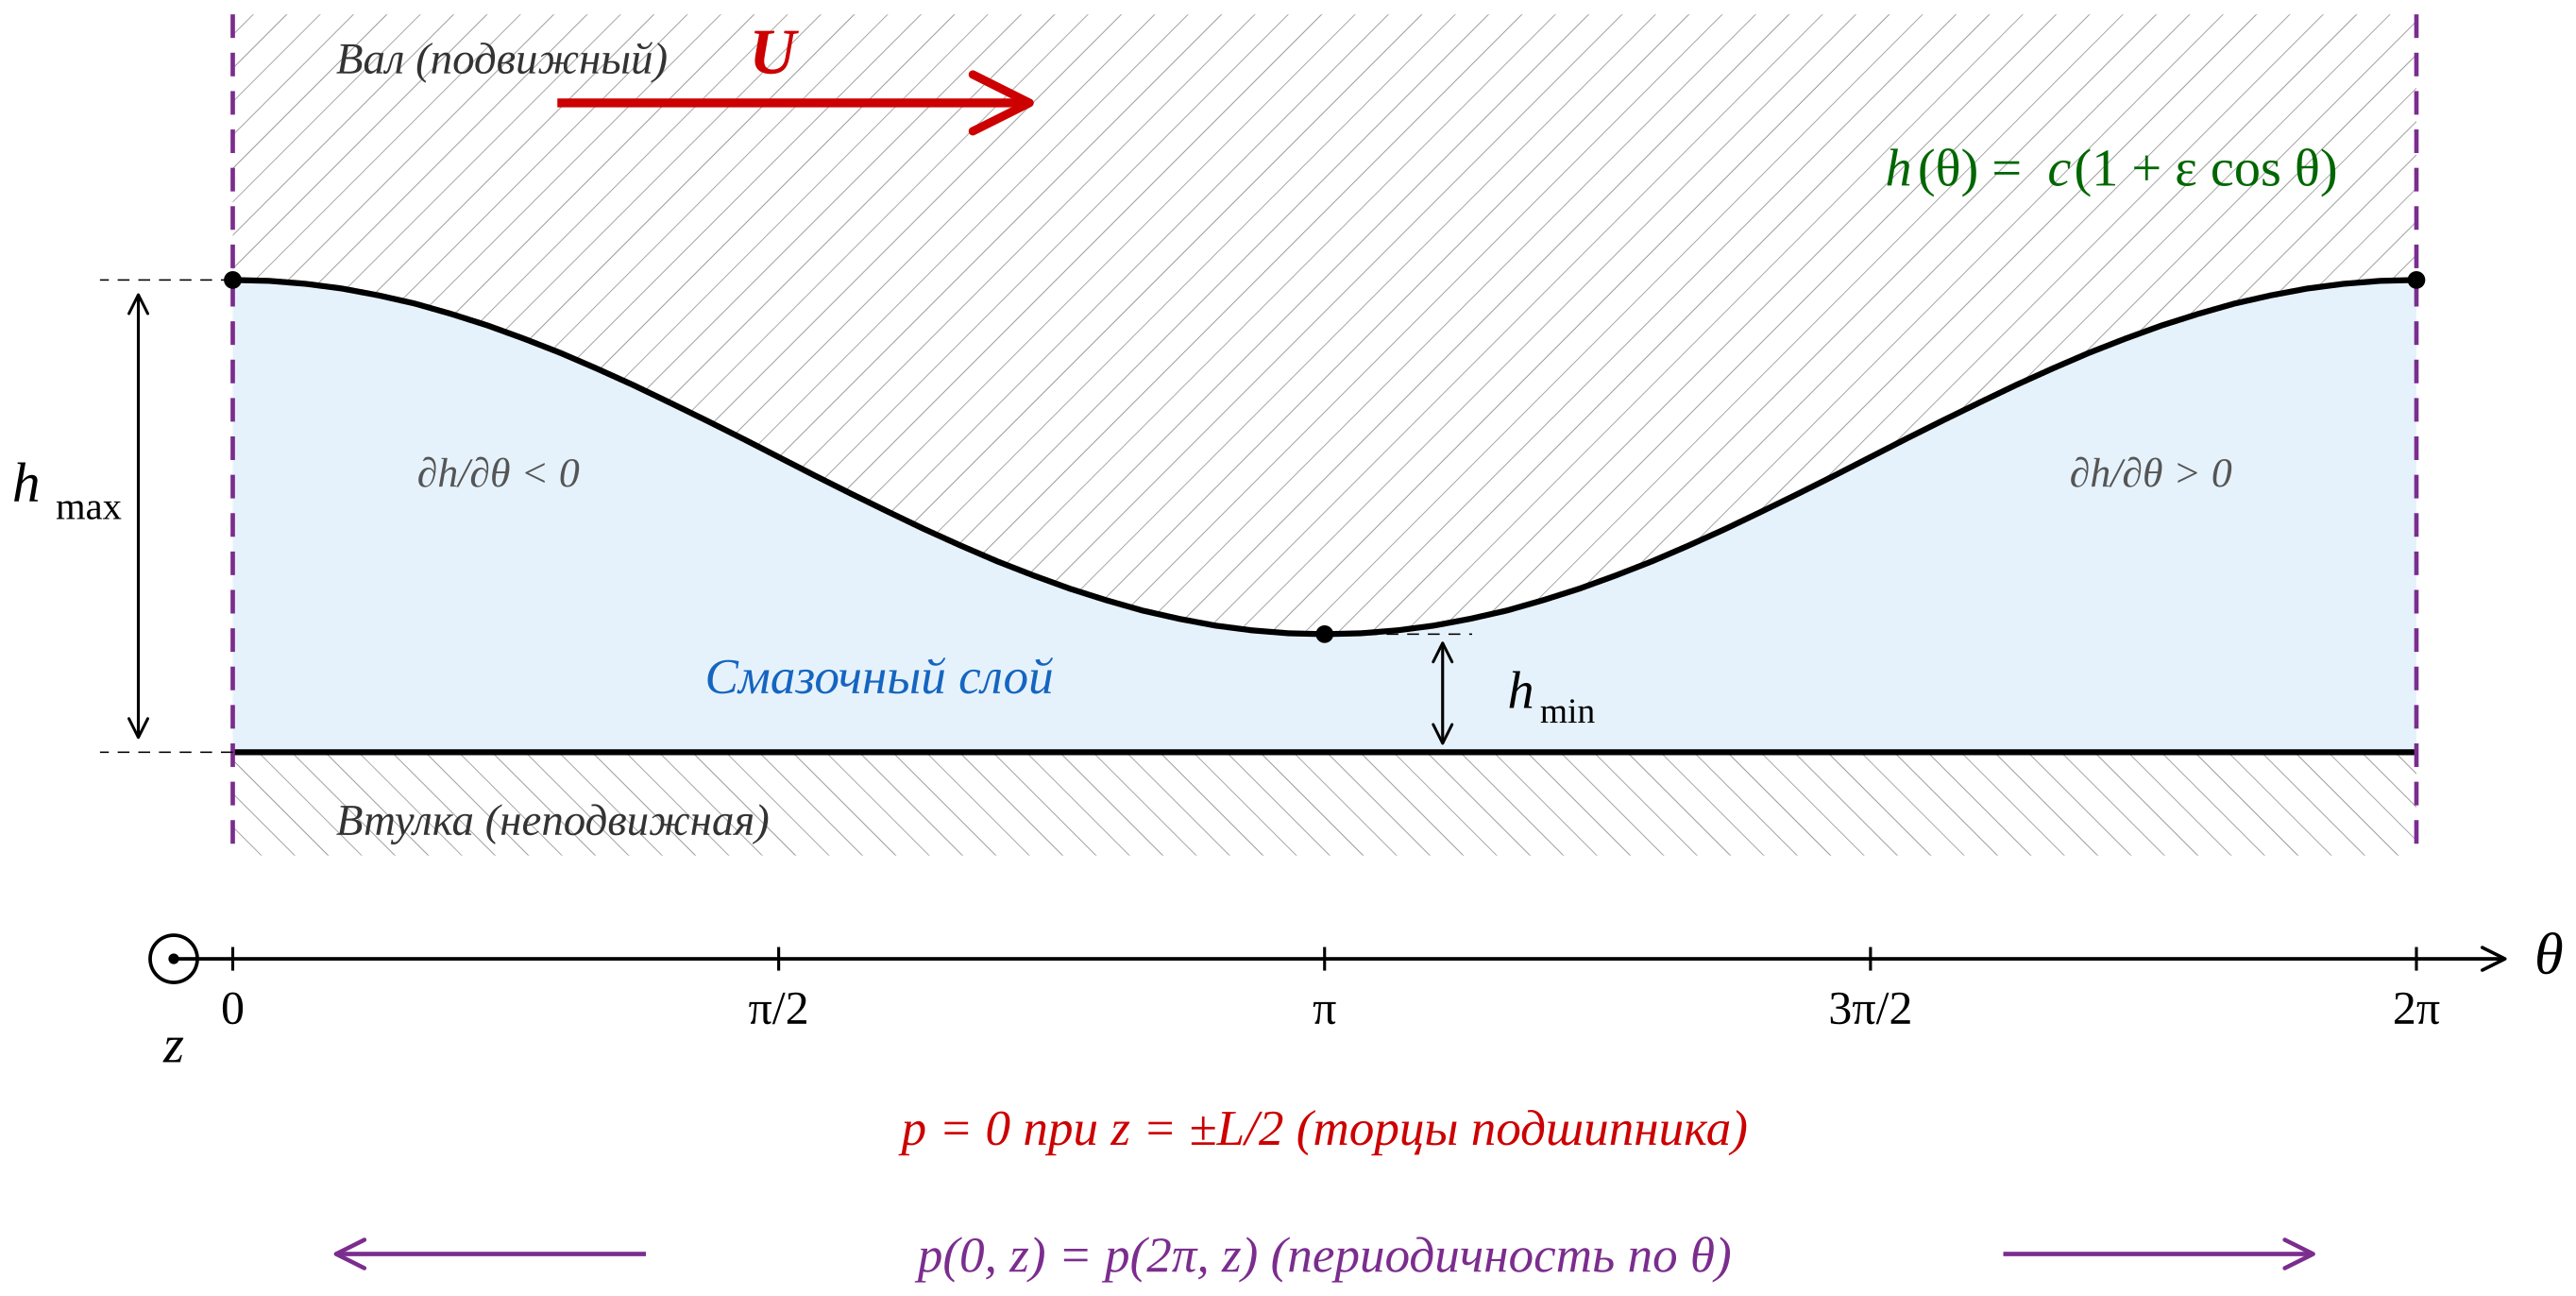
\includegraphics[width=\textwidth,height=0.9\textheight,keepaspectratio]{figures/ch02/fig_2_6.png}
\caption{Развёрнутый вид расчётной области радиального подшипника}
\label{fig:journal_unwrapped}
\end{figure}


\subsubsection*{Кинематика движения поверхностей}

Вал вращается с постоянной угловой скоростью~$\omega$ внутри неподвижной втулки. Окружная скорость поверхности вала составляет:
\begin{equation}
U = \omega\,R.
\label{eq:journal_U}
\end{equation}

Осевые скорости обеих поверхностей равны нулю. В стационарном режиме положение вала фиксировано: $\varepsilon = \mathrm{const}$, и нормальные скорости поверхностей обращаются в нуль, что исключает эффект выжимания ($\partial h/\partial t = 0$). При нестационарном анализе (динамика ротора) эксцентриситет $\varepsilon$ и угол нагрузки $\varphi$ зависят от времени, и в правой части уравнения Рейнольдса появляется squeeze-term $\partial h/\partial t$; такой случай выходит за рамки настоящего раздела.

Динамическая вязкость смазки полагается постоянной: $\mu = \mathrm{const}$ (допущение~6 из подраздела~2.1.1). Влияние температурной зависимости вязкости $\mu(T)$ рассматривается в главе~4.

Вращение вала создаёт увлекающий (куэттовский) поток смазки в окружном направлении. В зоне сходящегося зазора ($0 < \theta < \pi$, где толщина уменьшается от $h_{\max}$ к $h_{\min}$) условие неразрывности приводит к росту давления. В зоне расходящегося зазора ($\pi < \theta < 2\pi$) давление стремится к отрицательным значениям, однако физически отрицательное давление не реализуется: жидкость разрывается и образуется кавитационная зона. Именно сочетание клинового эффекта и кавитации определяет распределение давления и несущую способность радиального подшипника.


\subsubsection*{Закон толщины смазочного слоя}

Толщина смазочного слоя определяется геометрией двух эксцентричных цилиндров -- вала и втулки. При условии тонкого зазора ($c/R \ll 1$, что согласуется с допущением~3 из подраздела~2.1.1) и пренебрежении членами порядка $(c/R)^2$ и выше, толщина зазора записывается в виде:
\begin{equation}
h(\theta) = c\,(1 + \varepsilon\,\cos\theta),
\label{eq:journal_h}
\end{equation}
\begin{conditions}
$c = R_b - R$ -- радиальный зазор;\\
$\varepsilon = e/c$ -- относительный эксцентриситет.
\end{conditions}
Из формулы~\eqref{eq:journal_h} следует:
\begin{itemize}
\item максимальная толщина зазора $h_{\max} = c(1 + \varepsilon)$ достигается при $\theta = 0$ (точка, диаметрально противоположная минимальному зазору);
\item минимальная толщина зазора $h_{\min} = c(1 - \varepsilon)$ достигается при $\theta = \pi$ (точка наибольшего сближения вала и втулки).
\end{itemize}

Толщина зазора~\eqref{eq:journal_h} не зависит от осевой координаты~$z$, что соответствует осевой однородности геометрии (вал и втулка имеют цилиндрическую форму с параллельными осями). Зависимость $h$ от $z$ может возникать при перекосе вала (misalignment), однако этот случай в настоящей работе не рассматривается.

В общем случае, при наличии детерминированных микроструктур на рабочей поверхности, толщина смазочного слоя записывается как суперпозиция:
\begin{equation}
h(\theta, z) = c\,(1 + \varepsilon\,\cos\theta) + \Delta h(\theta, z),
\label{eq:journal_h_textured}
\end{equation}
где $\Delta h(\theta, z)$ -- добавка, описывающая геометрию микроструктуры (раздел~2.2).

Для характеристики геометрии радиального подшипника вводятся следующие безразмерные параметры:
\begin{itemize}
\item $\varepsilon = e/c$ -- относительный эксцентриситет, являющийся основным параметром нагружения ($\varepsilon = 0$ соответствует концентричному расположению, $\varepsilon \to 1$ -- контакту поверхностей);
\item $\psi = c/R$ -- относительный зазор (для типичных подшипников $\psi \sim 10^{-3}$);
\item $L/D$ -- отношение длины подшипника к диаметру ($D = 2R$), определяющее степень влияния осевых утечек: при $L/D > 1$ подшипник считается длинным, при $L/D < 0{,}5$ -- коротким, промежуточные значения соответствуют подшипнику конечной длины.
\end{itemize}


\subsubsection*{Уравнение Рейнольдса для радиального подшипника}

Обобщённое уравнение Рейнольдса~\eqref{eq:reynolds_full}, полученное в подразделе~2.1.1 в декартовых координатах, необходимо переписать для цилиндрической поверхности зазора радиального подшипника. Введём дуговую координату $x = R\theta$ (расстояние вдоль окружности вала), вдоль которой производная принимает вид $\partial/\partial x = (1/R)\,\partial/\partial\theta$. Осевая координата~$z$ остаётся без изменений.

В рассматриваемой задаче втулка неподвижна ($U_1 = 0$), вал движется с окружной скоростью $U_2 = \omega R = U$; осевые скорости обеих поверхностей равны нулю ($W_1 = W_2 = 0$). В стационарном режиме ($\partial h/\partial t = 0$) правая часть обобщённого уравнения Рейнольдса содержит единственный член:
\begin{equation}
\frac{U_1 + U_2}{2}\,\frac{1}{R}\,\frac{\partial h}{\partial \theta} = \frac{U}{2R}\,\frac{\partial h}{\partial \theta} = \frac{\omega}{2}\,\frac{\partial h}{\partial \theta}.
\label{eq:journal_rhs_derivation}
\end{equation}

Стационарное уравнение Рейнольдса для несжимаемой ньютоновской жидкости в координатах $(\theta, z)$ принимает вид:
\begin{equation}
\frac{1}{R^2}\frac{\partial}{\partial \theta}\!\left[\frac{h^3}{12\mu}\,\frac{\partial p}{\partial \theta}\right] + \frac{\partial}{\partial z}\!\left[\frac{h^3}{12\mu}\,\frac{\partial p}{\partial z}\right] = \frac{\omega}{2}\,\frac{\partial h}{\partial \theta}.
\label{eq:journal_reynolds}
\end{equation}

Множитель $1/R^2$ перед первым слагаемым в левой части обусловлен двукратным применением оператора $\partial/\partial x = (1/R)\,\partial/\partial\theta$ при переходе от декартовой координаты~$x$ к угловой~$\theta$.

Умножая обе части уравнения~\eqref{eq:journal_reynolds} на~$12\mu$ (что допустимо при $\mu = \mathrm{const}$), получаем эквивалентную форму, удобную для численной реализации:
\begin{equation}
\frac{1}{R^2}\frac{\partial}{\partial \theta}\!\left[h^3\,\frac{\partial p}{\partial \theta}\right] + \frac{\partial}{\partial z}\!\left[h^3\,\frac{\partial p}{\partial z}\right] = 6\mu\omega\,\frac{\partial h}{\partial \theta}.
\label{eq:journal_reynolds_num}
\end{equation}

Уравнение~\eqref{eq:journal_reynolds_num} является основным расчётным уравнением для радиального подшипника в настоящей работе.

Подставляя конкретное выражение для толщины зазора~\eqref{eq:journal_h}, получаем производную в правой части:
\begin{equation}
\frac{\partial h}{\partial \theta} = -c\,\varepsilon\,\sin\theta.
\label{eq:journal_dh_dtheta}
\end{equation}

Правая часть уравнения~\eqref{eq:journal_reynolds_num} принимает вид $-6\mu\omega\,c\,\varepsilon\,\sin\theta$. Источниковый член в правой части пропорционален $-\sin\theta$, поэтому максимум генерации давления приходится на $\theta \approx \pi/2$, где скорость сужения зазора наибольшая. В зоне $0 < \theta < \pi$ выполняется $\partial h/\partial\theta < 0$ (сходящийся клин): зазор уменьшается по направлению вращения, и давление генерируется. В зоне $\pi < \theta < 2\pi$ выполняется $\partial h/\partial\theta > 0$ (расходящийся клин): зазор увеличивается, давление стремится к отрицательным значениям, и вступает в действие кавитация.

Левая часть уравнений~\eqref{eq:journal_reynolds}-\eqref{eq:journal_reynolds_num} представляет собой эллиптический оператор $\nabla \cdot (h^3 \nabla p)$, записанный в координатах $(\theta, z)$ на цилиндрической поверхности. По структуре он аналогичен оператору в уравнении для упорного подшипника~\eqref{eq:thrust_reynolds_num}, однако здесь вместо координат $(r, \theta)$ используются $(\theta, z)$. Правая часть -- источниковый член, пропорциональный $\sin\theta$: максимум генерации давления приходится на $\theta = \pi/2$. При $\varepsilon = 0$ (концентричное расположение вала и втулки) $\partial h/\partial \theta = 0$, правая часть обращается в нуль и давление не генерируется -- подшипник не несёт нагрузки.

Уравнение~\eqref{eq:journal_reynolds_num} допускает два классических предельных случая, для которых известны аналитические решения.

\textit{Бесконечно длинный подшипник ($L/D \to \infty$).} В этом пределе давление не зависит от осевой координаты: $\partial p/\partial z = 0$, и уравнение~\eqref{eq:journal_reynolds_num} вырождается в обыкновенное дифференциальное уравнение по~$\theta$. Полное аналитическое решение этого ОДУ с периодическими граничными условиями и без учёта кавитации известно как решение Зоммерфельда (Sommerfeld, 1904). Учёт кавитации приводит к половинному решению (half-Sommerfeld), в котором давление обнуляется в зоне расходящегося зазора.

\textit{Бесконечно короткий подшипник ($L/D \to 0$).} В этом пределе осевой градиент давления значительно превышает окружной: $\partial^2 p/\partial z^2 \gg (1/R^2)\,\partial^2 p/\partial \theta^2$, и окружной член в левой части уравнения~\eqref{eq:journal_reynolds_num} может быть опущен. Уравнение вырождается в ОДУ по~$z$ при каждом фиксированном~$\theta$, что допускает аналитическое решение. Это приближение известно как приближение Дюбуа--Оквирка (Dubois--Ocvirk, short-bearing approximation) и даёт удовлетворительные результаты при $L/D < 0{,}5$.

Для подшипника конечной длины ($0{,}5 \lesssim L/D \lesssim 2$) ни один из предельных случаев не обеспечивает достаточной точности, и уравнение~\eqref{eq:journal_reynolds_num} решается численно (глава~3).


\subsubsection*{Граничные условия}

Для замыкания уравнения Рейнольдса~\eqref{eq:journal_reynolds_num} необходимо задать граничные условия на давление по всему контуру расчётной области~\eqref{eq:journal_domain}.

\textit{По окружной координате~$\theta$.} Область по~$\theta$ охватывает полную окружность, поэтому естественным условием является периодичность:
\begin{equation}
p(0, z) = p(2\pi, z), \quad \frac{\partial p}{\partial \theta}\bigg|_{\theta=0} = \frac{\partial p}{\partial \theta}\bigg|_{\theta=2\pi}.
\label{eq:journal_bc_periodic}
\end{equation}

\textit{По осевой координате~$z$.} На торцах подшипника давление принимается равным атмосферному:
\begin{equation}
p(\theta,\,-L/2) = 0, \quad p(\theta,\,L/2) = 0,
\label{eq:journal_bc_axial}
\end{equation}
где давление отсчитывается от атмосферного ($p = p_{\mathrm{abs}} - p_{\mathrm{atm}}$), как и в подразделе~2.1.2. При наличии принудительной подачи смазки через осевую канавку условие на соответствующем угле $\theta = \theta_{\mathrm{groove}}$ модифицируется: $p(\theta_{\mathrm{groove}}, z) = p_{\mathrm{sup}}$, где $p_{\mathrm{sup}}$ -- давление подачи. Помимо условий Дирихле на торцах, в специальных конструкциях могут применяться условия непротекания $q_z = 0$, эквивалентные $\partial p/\partial z = 0$ (при наличии уплотнений на торцах подшипника), или смешанные условия, когда на части окружности задаётся давление подачи, а на остальной -- атмосферное давление.

\textit{Кавитация.} Принципиальной особенностью радиального подшипника является неизбежное возникновение кавитации в зоне расходящегося зазора ($\pi < \theta < 2\pi$), где расчётное давление стремится к отрицательным значениям. В простейшей постановке применяют ограничение $p \geq 0$ (условие Гюмбеля), при котором отрицательные давления обнуляются после решения. Более физичным является условие Рейнольдса (Swift--Stieber), требующее одновременного выполнения $p = 0$ и $\partial p/\partial \theta = 0$ на границе кавитации. Оба подхода, однако, не обеспечивают точного сохранения массы. Корректная массо-сохраняющая постановка, основанная на модели Jakobsson--Floberg--Olsson (JFO), вводится в разделе~2.3.

Граница кавитационной зоны является внутренней границей задачи, положение которой заранее неизвестно и определяется в процессе решения. Периодичность задаётся как граничное условие на контуре области~\eqref{eq:journal_domain}, а кавитационная зона является внутренней частью решения. Само поле давления $p(\theta, z)$ при этом остаётся непрерывным и периодическим, хотя и состоит из двух участков: зоны полного смазочного слоя ($p > 0$) и зоны кавитации ($p = 0$). Качественное распределение давления $p(\theta)$ в среднем сечении подшипника ($z = 0$) показано на рисунке~\ref{fig:journal_pressure_profile}.

% [РИСУНОК: Качественный профиль давления в радиальном подшипнике]
% Должен показывать:
% - Ось абсцисс: θ от 0 до 2π
% - p(θ) при z=0: рост в зоне 0 < θ < π, максимум вблизи θ = π/2
% - Зона кавитации: p = 0 при π < θ < 2π (приблизительно)
% - Границы разрыва и восстановления
% - Пунктир: полное решение Зоммерфельда (без кавитации, отрицательные давления)
\begin{figure}[!ht]
\centering
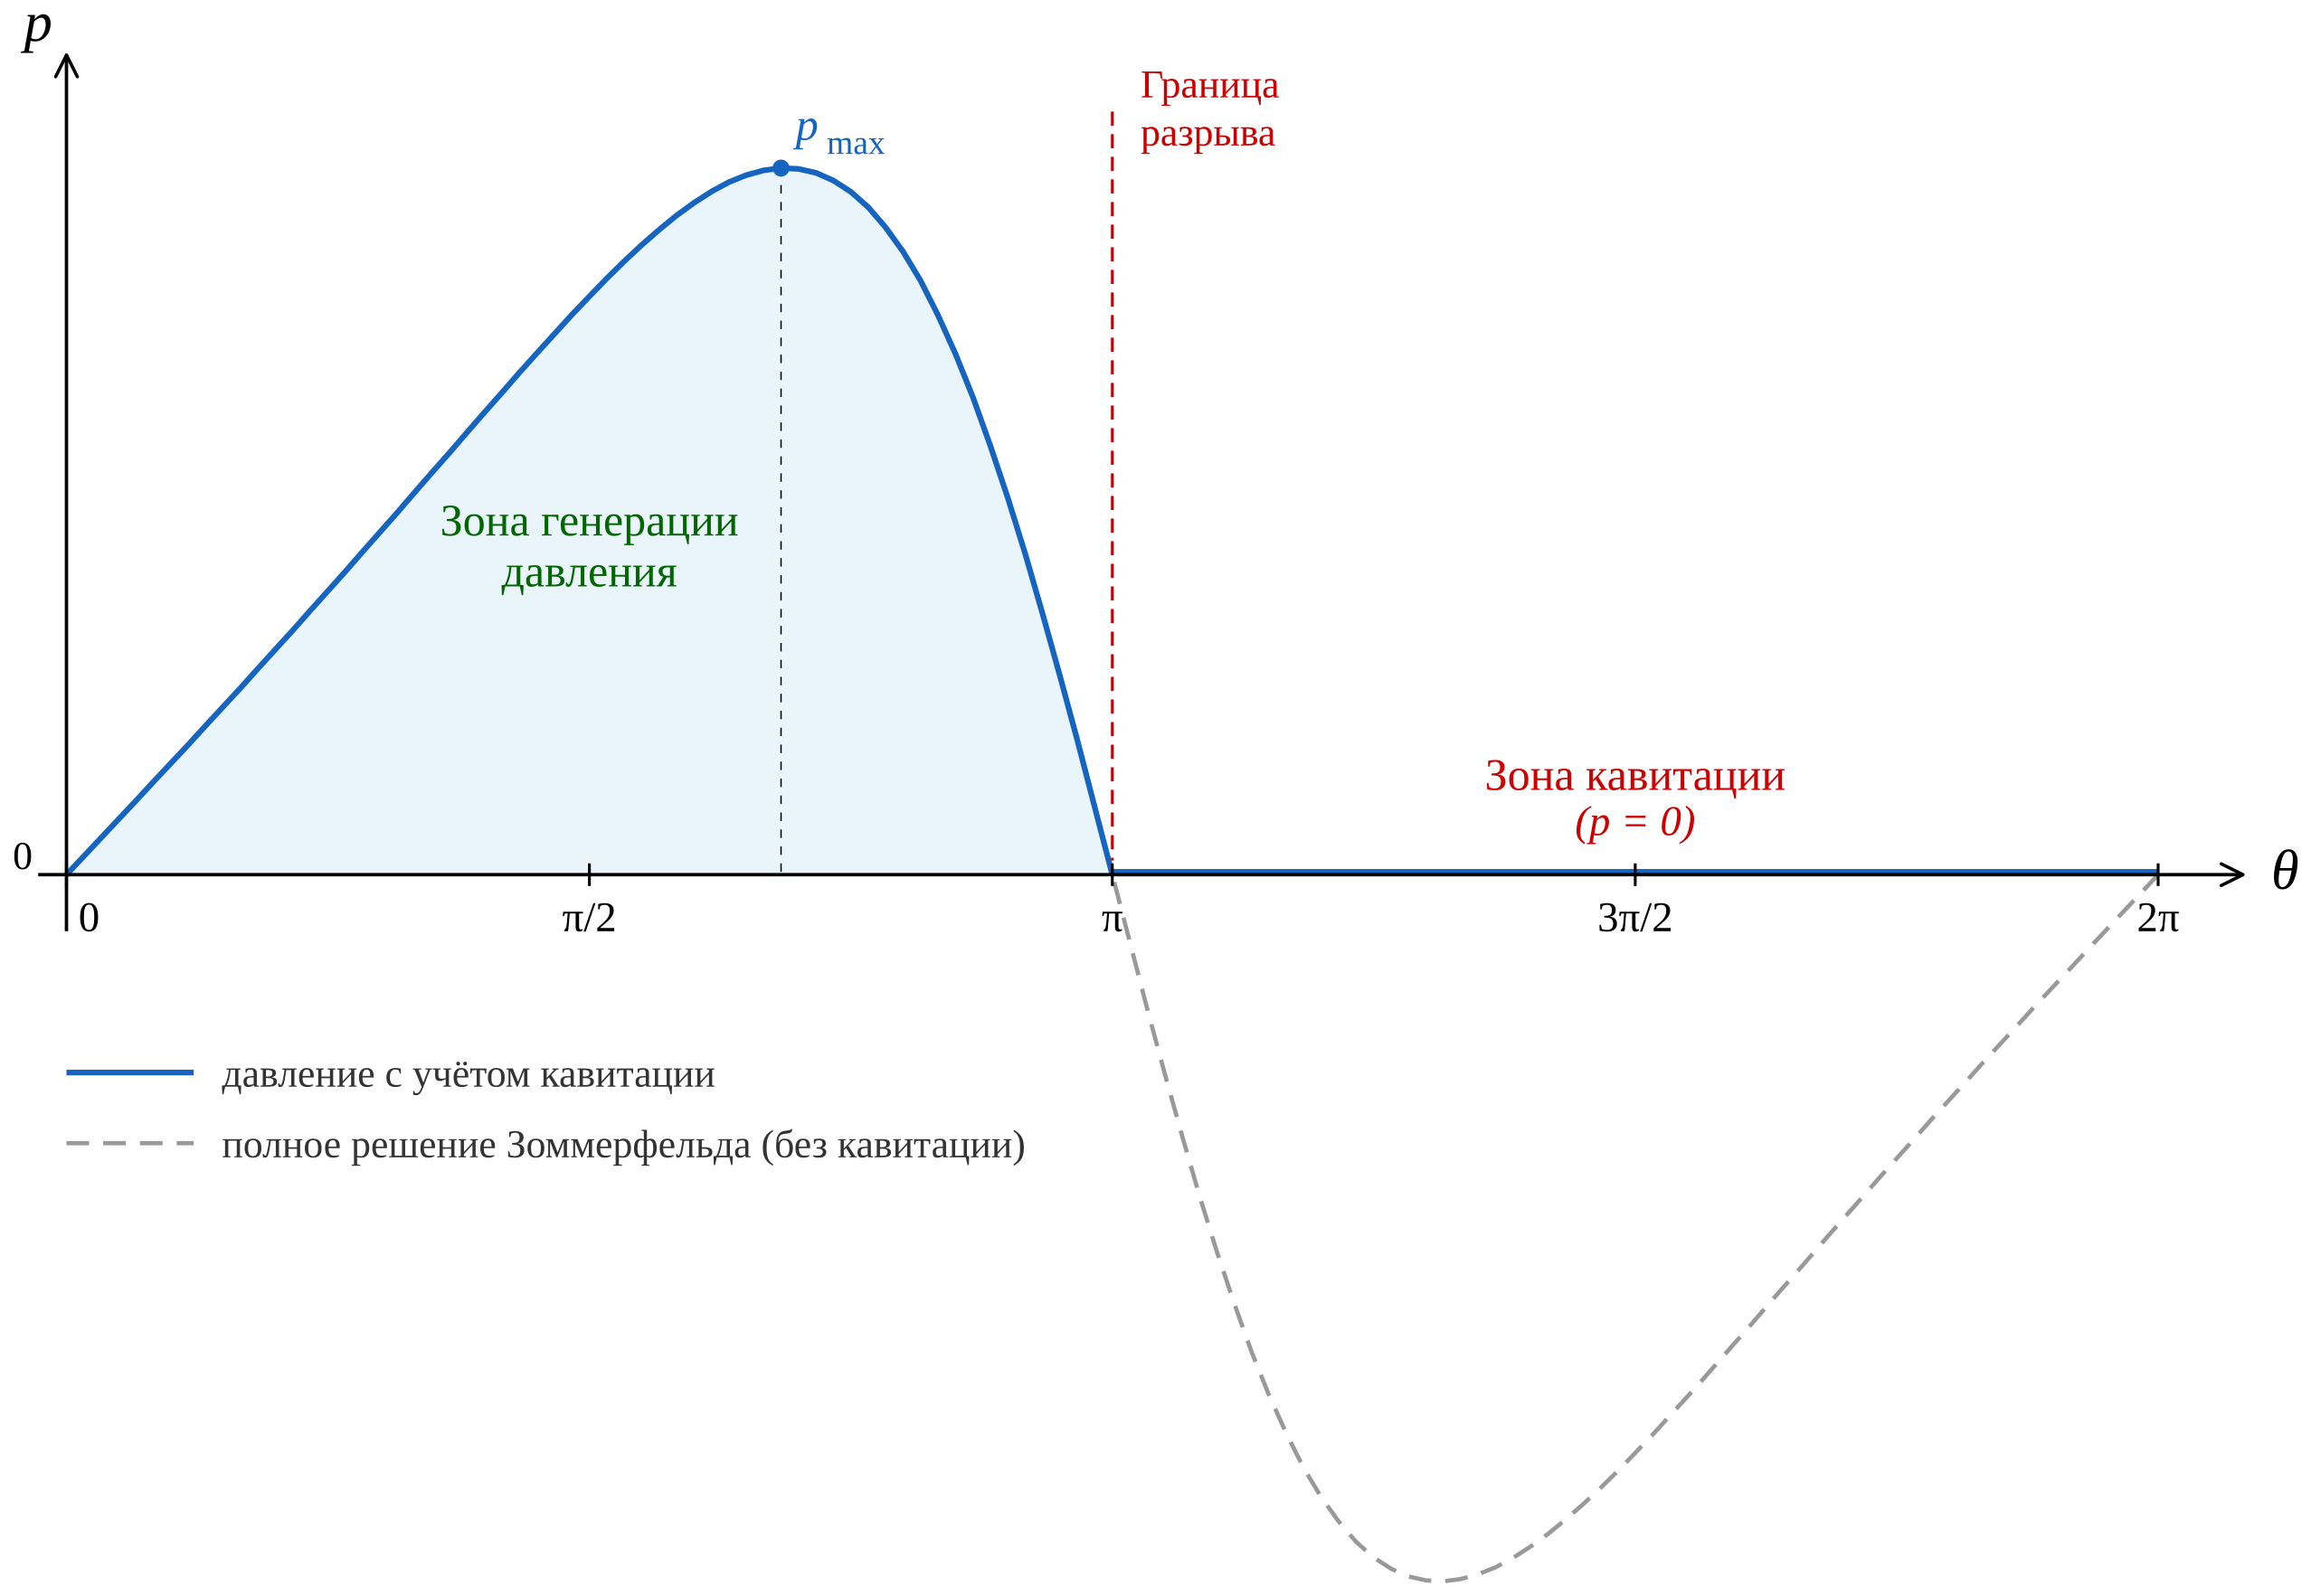
\includegraphics[width=\textwidth,height=0.9\textheight,keepaspectratio]{figures/ch02/fig_2_7.png}
\caption{Качественное распределение давления в радиальном подшипнике и зона кавитации}
\label{fig:journal_pressure_profile}
\end{figure}


\subsubsection*{Объёмные расходы}

Объёмные расходы жидкости через единицу длины определяются путём интегрирования профилей скорости по толщине смазочного слоя, аналогично подразделу~2.1.2.

Окружной расход (на единицу длины по осевой координате~$z$):
\begin{equation}
\label{eq:journal_q_theta}
q_\theta(\theta, z) = \frac{h\,U}{2} - \frac{h^3}{12\mu\,R}\,\frac{\partial p}{\partial \theta} = \frac{h\,\omega R}{2} - \frac{h^3}{12\mu\,R}\,\frac{\partial p}{\partial \theta}.
\end{equation}

Первое слагаемое представляет куэттовскую составляющую расхода, обусловленную увлечением жидкости вращающимся валом; второе -- пуазейлевскую составляющую, определяемую окружным градиентом давления. Множитель $1/R$ во втором слагаемом обусловлен переходом от производной по дуге $\partial/\partial(R\theta)$ к производной по углу $\partial/\partial\theta$.

Осевой расход (на единицу длины по окружной координате):
\begin{equation}
q_z(\theta, z) = -\frac{h^3}{12\mu}\,\frac{\partial p}{\partial z}.
\label{eq:journal_q_z}
\end{equation}

Поскольку осевые скорости обеих поверхностей равны нулю, осевой расход полностью определяется градиентом давления (пуазейлевская составляющая). Именно осевой расход обусловливает боковую утечку смазки через торцы подшипника.

Суммарная утечка через торцы подшипника определяется интегрированием осевого расхода по окружности:
\begin{equation}
Q_{\mathrm{side}} = \int_0^{2\pi} \bigl[ q_z(\theta,\,L/2) - q_z(\theta,\,-L/2) \bigr]\,R\,\mathrm{d}\theta.
\label{eq:journal_Q_side}
\end{equation}

Множитель $R\,\mathrm{d}\theta$ соответствует элементу длины дуги на окружности вала. Здесь $q_z(\theta, L/2) > 0$ соответствует потоку, вытекающему через торец $z = L/2$ (по направлению внешней нормали $+\mathbf{e}_z$), а $q_z(\theta, -L/2) < 0$ -- потоку, вытекающему через торец $z = -L/2$ (нормаль $-\mathbf{e}_z$). Обозначая утечки через отдельные торцы как $Q_+ = \int_0^{2\pi} q_z(\theta, L/2)\,R\,\mathrm{d}\theta$ и $Q_- = -\int_0^{2\pi} q_z(\theta, -L/2)\,R\,\mathrm{d}\theta$, получаем $Q_{\mathrm{side}} = Q_+ + Q_-$.

При симметрии давления относительно средней плоскости подшипника ($p(\theta, z) = p(\theta, -z)$) утечки через оба торца одинаковы, и выражение~\eqref{eq:journal_Q_side} упрощается:
\begin{equation}
Q_{\mathrm{side}} = 2\int_0^{2\pi} q_z(\theta,\,L/2)\,R\,\mathrm{d}\theta.
\label{eq:journal_Q_side_sym}
\end{equation}

Боковая утечка является основным механизмом потери смазки в радиальном подшипнике. При уменьшении отношения $L/D$ доля давления, <<разгружаемая>> через торцы, возрастает, что снижает несущую способность. В предельном случае бесконечно короткого подшипника ($L/D \to 0$) осевые утечки полностью доминируют, и именно это обстоятельство позволяет пренебречь окружным членом в уравнении Рейнольдса (приближение Дюбуа--Оквирка).

Баланс массы в стационарном режиме без выжимания записывается в дифференциальной форме (аналогично уравнению~\eqref{eq:thrust_mass_balance} для упорного подшипника):
\begin{equation}
\frac{1}{R}\,\frac{\partial q_\theta}{\partial \theta} + \frac{\partial q_z}{\partial z} = 0.
\label{eq:journal_mass_balance}
\end{equation}

Подстановка выражений~\eqref{eq:journal_q_theta} и~\eqref{eq:journal_q_z} в уравнение~\eqref{eq:journal_mass_balance} приводит к уравнению Рейнольдса~\eqref{eq:journal_reynolds}.


Решение уравнения Рейнольдса даёт поле давления~$p$ в расчётной области. По найденному давлению вычисляются интегральные характеристики узла: несущая способность, расходы смазки, силы и моменты трения, минимальная толщина плёнки. Унифицированные формулы для всех выходных величин приведены в подразделе~2.1.7.

В практической постановке задачи внешняя радиальная нагрузка $\mathbf{W}_{\mathrm{ext}}$ и параметры режима ($\omega$, $\mu$, $c$, $R$, $L$) считаются заданными, тогда как положение вала $(\varepsilon, \varphi)$ является неизвестным. Равновесное положение определяется из условия статического баланса сил: $\mathbf{W}(\varepsilon, \varphi) = -\mathbf{W}_{\mathrm{ext}}$, т.\,е. из системы двух нелинейных уравнений относительно $\varepsilon$ и $\varphi$. Численное решение этой системы методом итерационного поиска описывается в главе~3.

Сформулированная задача сводится к решению эллиптического уравнения Рейнольдса~\eqref{eq:journal_reynolds_num} в прямоугольной области~\eqref{eq:journal_domain} с периодическими условиями по окружной координате~$\theta$ и условиями Дирихле по осевой координате~$z$. Принципиальной особенностью радиального подшипника, отличающей его от упорного (подраздел~2.1.2), является неизбежное возникновение кавитации в зоне расходящегося зазора: при любом ненулевом эксцентриситете $\varepsilon > 0$ правая часть уравнения Рейнольдса меняет знак, и в отсутствие ограничений на давление решение содержит области с $p < 0$~\cite{gao2014}.

Численная дискретизация уравнения~\eqref{eq:journal_reynolds_num} методом конечных разностей и алгоритм учёта кавитации на основе модели JFO рассматриваются в главе~3. При наличии микроструктур на рабочей поверхности функция зазора~\eqref{eq:journal_h_textured} приобретает быстрые локальные вариации, параметризация которых описывается в разделе~2.2.

\FloatBarrier
\subsection{Постановка задачи для радиального зазора при возвратно-поступательном движении}

Рассмотрим узел трения с осевым возвратно-поступательным относительным движением поверхностей: плунжер (поршень, шток) совершает возвратно-поступательное перемещение внутри цилиндра (втулки). Тонкий слой вязкой жидкости заполняет кольцевой зазор между сопряжёнными цилиндрическими поверхностями и выполняет функцию смазки и уплотнения.

Узлы данного типа широко распространены в машиностроении. В плунжерных насосах высокого давления зазор между плунжером и гильзой одновременно уплотняет рабочую жидкость и обеспечивает смазку. В гидроцилиндрах поршень перемещается внутри гильзы под действием давления рабочей жидкости. В поршневых компрессорах и двигателях внутреннего сгорания поршень с кольцами образует трибологическую пару скольжения с гильзой цилиндра. В направляющих скольжения металлорежущих станков возвратно-поступательное движение суппорта или стола сопровождается формированием смазочного слоя~\cite{hori2002,szeri1998}.

Ключевое отличие рассматриваемой постановки от подразделов~2.1.2-2.1.3 состоит в следующем. Скорость увлечения $U(t)$ меняет знак при реверсе хода, вследствие чего клиновой член в правой части уравнения Рейнольдса меняет знак: зона повышенного давления <<переезжает>> от одного конца рабочей зоны к другому. При каждом реверсе возможны разрыв и последующее восстановление сплошности смазочного слоя. Второе существенное отличие -- нестационарный squeeze-член $\partial h/\partial t$ зачастую играет определяющую роль: колебания эксцентриситета, вибрации и перекос плунжера приводят к изменению зазора во времени, что генерирует давление даже при отсутствии клинового эффекта. Все общие допущения, принятые при выводе уравнения Рейнольдса, наследуются из подраздела~2.1.1.


\subsubsection*{Геометрия и система координат}

Основными геометрическими параметрами узла являются:
\begin{itemize}
\item $R$ -- радиус плунжера;
\item $R_b$ -- радиус внутренней поверхности цилиндра (втулки);
\item $c = R_b - R$ -- радиальный зазор;
\item $L$ -- длина рабочей зоны контакта (длина втулки);
\item $e(t)$ -- эксцентриситет (расстояние между осями плунжера и цилиндра), в общем случае зависящий от времени;
\item $\varepsilon(t) = e(t)/c$ -- относительный эксцентриситет;
\item $\varphi(t)$ -- угол положения линии центров.
\end{itemize}

Для описания задачи используется цилиндрическая система координат $(\theta, z, y)$:
\begin{itemize}
\item $z$ -- ось движения плунжера (вдоль хода), $z \in [0,\; L]$;
\item $\theta$ -- окружная координата, $\theta \in [0,\; 2\pi]$;
\item $y$ -- координата по толщине смазочного слоя, направленная от поверхности цилиндра ($y = 0$) к поверхности плунжера ($y = h$).
\end{itemize}

Область расчёта представляет собой прямоугольник:
\begin{equation}
\theta \in [0,\; 2\pi], \quad z \in [0,\; L].
\label{eq:recip_domain}
\end{equation}

В отличие от радиального подшипника (подраздел~2.1.3), где основное течение является окружным ($\theta$-направление), вызванным вращением вала, а утечка -- осевой ($z$), в возвратно-поступательном узле картина обратная: основное течение направлено вдоль оси $z$ и вызвано поступательным движением плунжера, а окружное течение является вторичным, обусловленным неоднородностью давления по~$\theta$. Схема узла представлена на рис.~\ref{fig:recip_scheme}.

% [РИСУНОК: Схема возвратно-поступательного узла]
\begin{figure}[!ht]
\centering
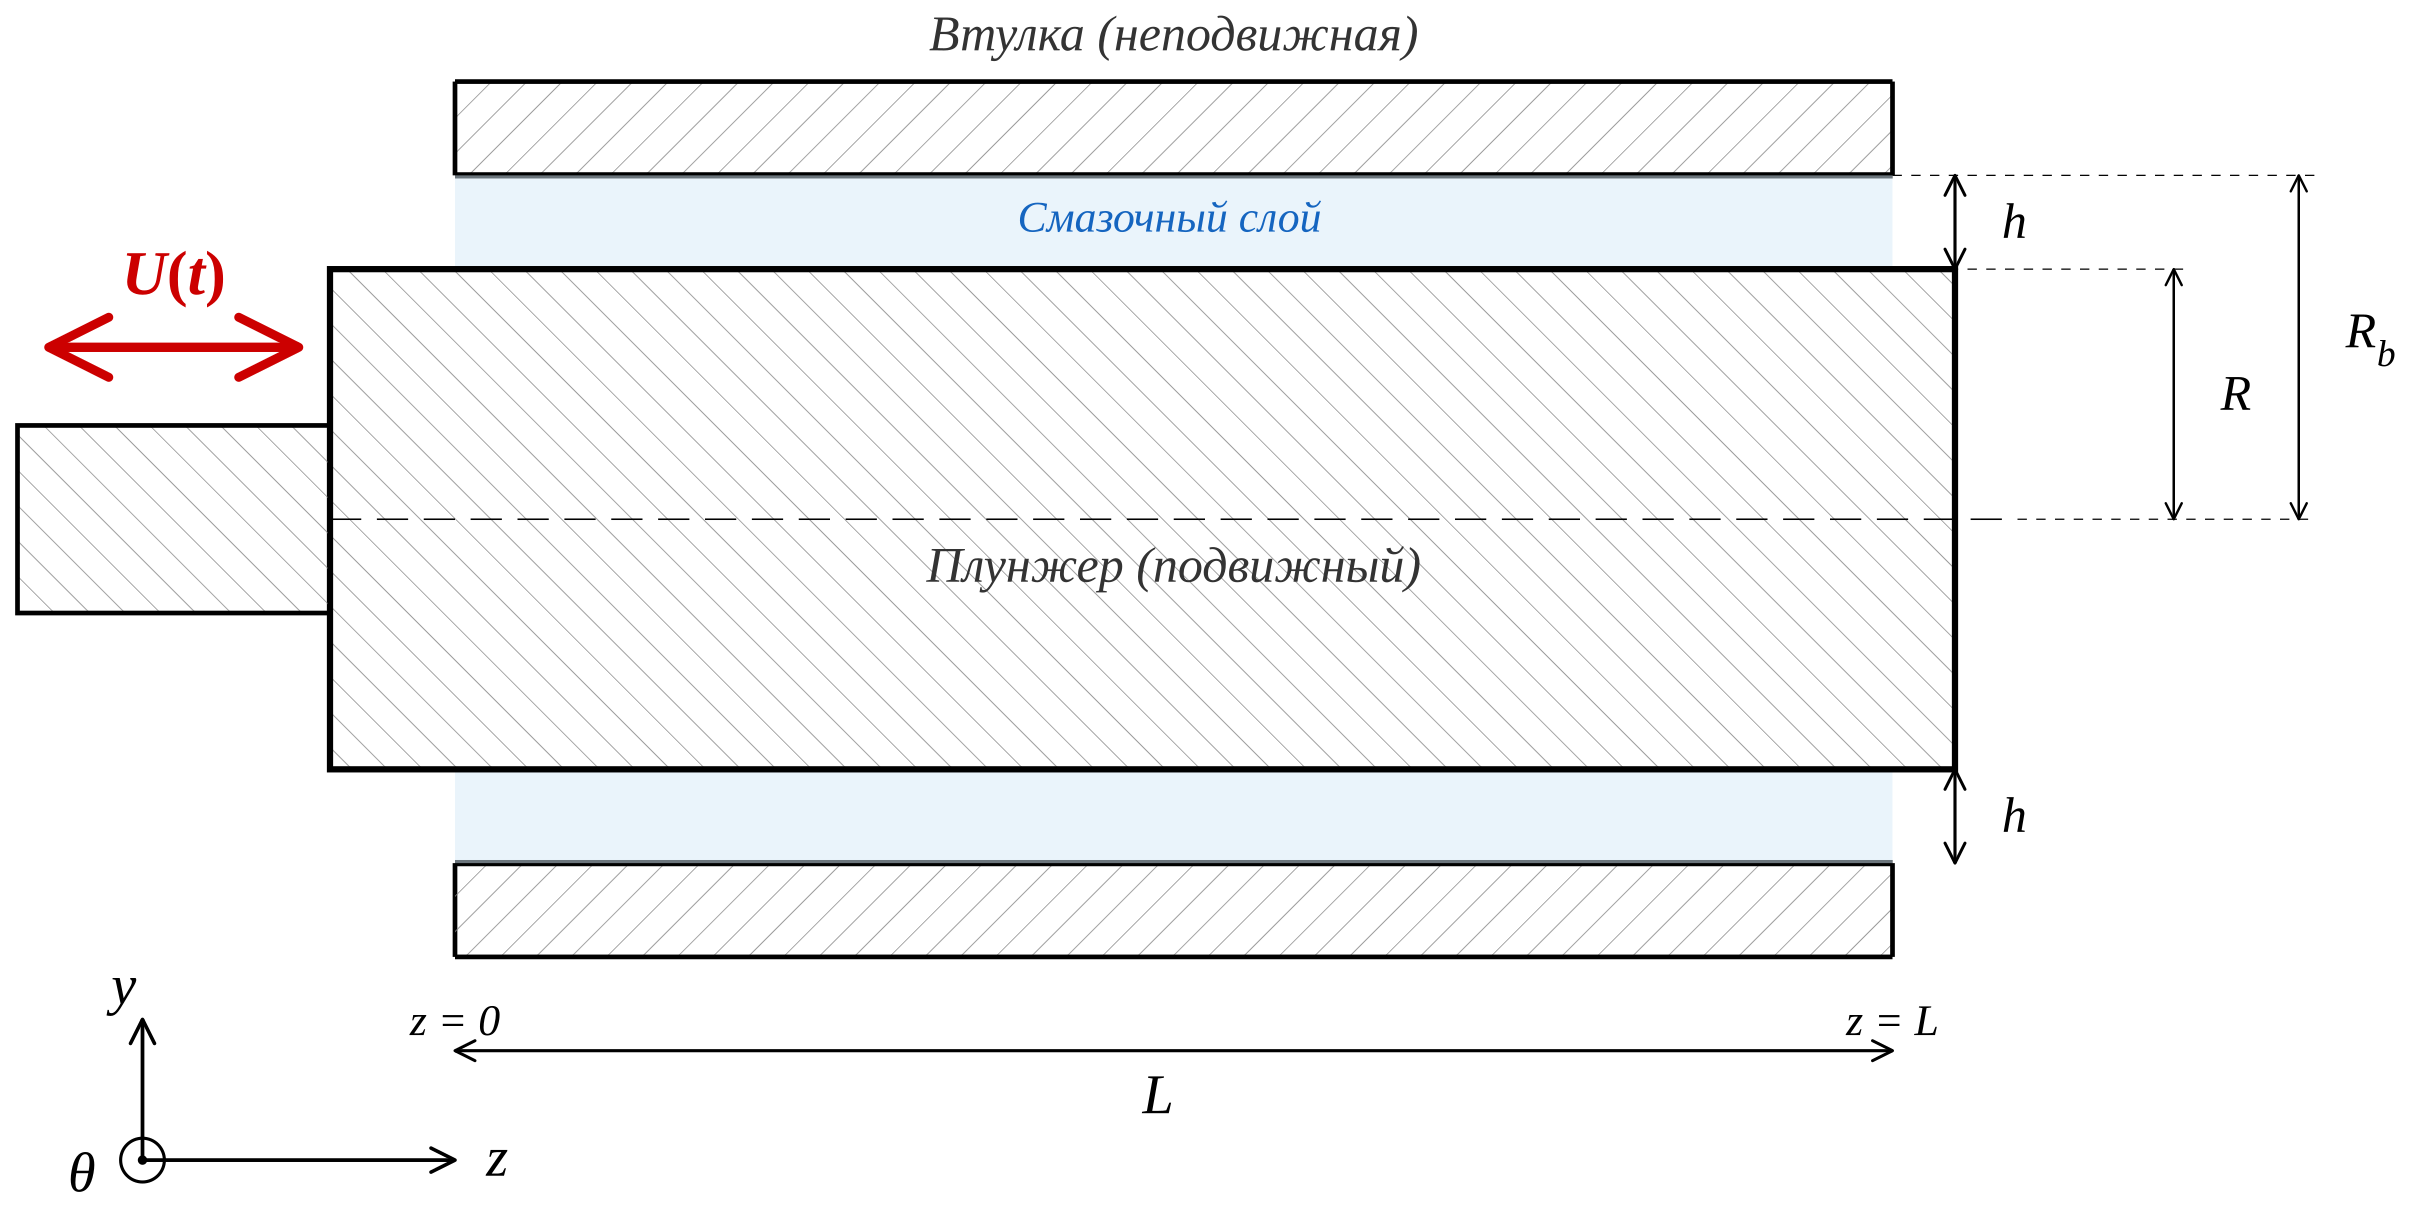
\includegraphics[width=\textwidth,height=0.9\textheight,keepaspectratio]{figures/ch02/fig_2_8.png}
\caption{Схема возвратно-поступательного узла: плунжер внутри цилиндрической втулки}
\label{fig:recip_scheme}
\end{figure}


\subsubsection*{Кинематика движения}

Закон хода плунжера задаётся функцией положения $s(t)$; скорость поступательного движения определяется как
\begin{equation}
U(t) = \frac{ds}{dt}.
\label{eq:recip_U}
\end{equation}

Типичный гармонический закон хода, удобный для верификации численных схем:
\begin{equation}
s(t) = \frac{S}{2}\bigl(1 - \cos(\Omega t)\bigr), \quad
U(t) = \frac{S\,\Omega}{2}\sin(\Omega t),
\label{eq:recip_harmonic}
\end{equation}
\begin{conditions}
$S$ -- полный ход (stroke);\\
$\Omega$ -- угловая частота возвратно-поступательного движения.
\end{conditions}
В реальных механизмах закон $s(t)$ может определяться кинематикой кривошипно-шатунного механизма, однако для модели достаточно задать $U(t)$ произвольной функцией времени.


\subsubsection*{Закон толщины смазочного слоя}

Базовая геометрия описывается двумя эксцентричными цилиндрами -- плунжером и втулкой, аналогично радиальному подшипнику (подраздел~2.1.3):
\begin{equation}
h(\theta, t) = c\bigl(1 + \varepsilon(t)\cos(\theta - \varphi(t))\bigr).
\label{eq:recip_h_base}
\end{equation}

Для возникновения клинового эффекта вдоль оси~$z$ необходима неоднородность $\partial h/\partial z \neq 0$. Источниками такой неоднородности являются: конусность (taper) зазора, перекос оси плунжера, микропрофиль поверхности, а также специально введённый рельеф (микротекстура, см.\ раздел~2.2).

Общий вид толщины зазора с учётом осевой конусности:
\begin{equation}
h(\theta, z, t) = c\bigl(1 + \varepsilon(t)\cos(\theta - \varphi(t))\bigr) + \kappa\Bigl(z - \frac{L}{2}\Bigr),
\label{eq:recip_h_tilt}
\end{equation}
где $\kappa$ -- параметр осевой конусности зазора (taper). При $\kappa > 0$ зазор увеличивается от середины к торцу $z = L$; при $\kappa < 0$ -- уменьшается. При $\kappa = 0$ клин вдоль $z$ отсутствует; давление может генерироваться только через squeeze-член ($\partial h/\partial t \neq 0$).
Параметры $\varepsilon$ и $\kappa$ должны удовлетворять условию $h(\theta, z, t) > 0$ по всей расчётной области; в частности, необходимо $\varepsilon < 1$ и $|\kappa|\,L/2 < c\,(1 - \varepsilon)$.

При наличии детерминированных микроструктур на рабочей поверхности толщина зазора записывается как суперпозиция:
\begin{equation}
h(\theta, z, t) = h_{\mathrm{base}}(\theta, z, t) + \Delta h(\theta, z),
\label{eq:recip_h_textured}
\end{equation}
где $\Delta h(\theta, z)$ -- добавка, описывающая геометрию микроструктуры (подробно в разделе~2.2).

Производная по времени от базового зазора~\eqref{eq:recip_h_tilt} при постоянной конусности ($\kappa = \mathrm{const}$) определяется изменением эксцентриситета и угла линии центров:
\begin{equation}
\frac{\partial h}{\partial t}
= c\bigl[\dot{\varepsilon}(t)\cos(\theta - \varphi(t))
       + \varepsilon(t)\,\dot{\varphi}(t)\sin(\theta - \varphi(t))\bigr],
\label{eq:recip_dhdt}
\end{equation}
\begin{conditions}
$\dot{\varepsilon} = d\varepsilon/dt$;\\
$\dot{\varphi} = d\varphi/dt$.
\end{conditions}
Слагаемое с конусностью $\kappa$ не вносит вклада в $\partial h/\partial t$, поскольку $\kappa$ не зависит от времени. При фиксированном положении плунжера ($\dot{\varepsilon} = 0$, $\dot{\varphi} = 0$) squeeze-член обращается в нуль, и давление генерируется только клиновым эффектом.


\subsubsection*{Уравнение Рейнольдса}

На цилиндрической поверхности зазора в координатах $(\theta, z)$ при осевом увлечении со скоростью $U(t)$ и отсутствии окружного увлечения уравнение Рейнольдса для несжимаемой ньютоновской жидкости принимает вид:
\begin{equation}
\frac{1}{R^2}\frac{\partial}{\partial\theta}
  \biggl(\frac{h^3}{12\mu}\frac{\partial p}{\partial\theta}\biggr)
+ \frac{\partial}{\partial z}
  \biggl(\frac{h^3}{12\mu}\frac{\partial p}{\partial z}\biggr)
= \frac{U(t)}{2}\frac{\partial h}{\partial z}
+ \frac{\partial h}{\partial t}.
\label{eq:recip_reynolds}
\end{equation}
Здесь $R$ -- радиус плунжера; ввиду малости зазора ($c \ll R$) замена $R$ на $R_b$ не вносит существенной погрешности.

Умножая обе части на~$12\mu$, получаем эквивалентную форму, удобную для численной реализации:
\begin{equation}
\frac{1}{R^2}\frac{\partial}{\partial\theta}
  \biggl(h^3\frac{\partial p}{\partial\theta}\biggr)
+ \frac{\partial}{\partial z}
  \biggl(h^3\frac{\partial p}{\partial z}\biggr)
= 6\mu\,U(t)\frac{\partial h}{\partial z}
+ 12\mu\frac{\partial h}{\partial t}.
\label{eq:recip_reynolds_num}
\end{equation}

Правая часть уравнения~\eqref{eq:recip_reynolds_num} содержит два слагаемых различной физической природы.

Первый член $6\mu\,U(t)\,\partial h/\partial z$ описывает клиновой эффект: давление генерируется при наличии сужения зазора вдоль направления движения ($\partial h/\partial z \neq 0$). При реверсе хода ($U < 0$) знак этого члена меняется на противоположный, и область повышенного давления <<переезжает>> от одного конца рабочей зоны к другому (рис.~\ref{fig:recip_reversal}). Именно этот механизм определяет несущую способность клинового зазора.

% [РИСУНОК: Реверс зоны давления при смене знака U(t)]
\begin{figure}[!ht]
\centering
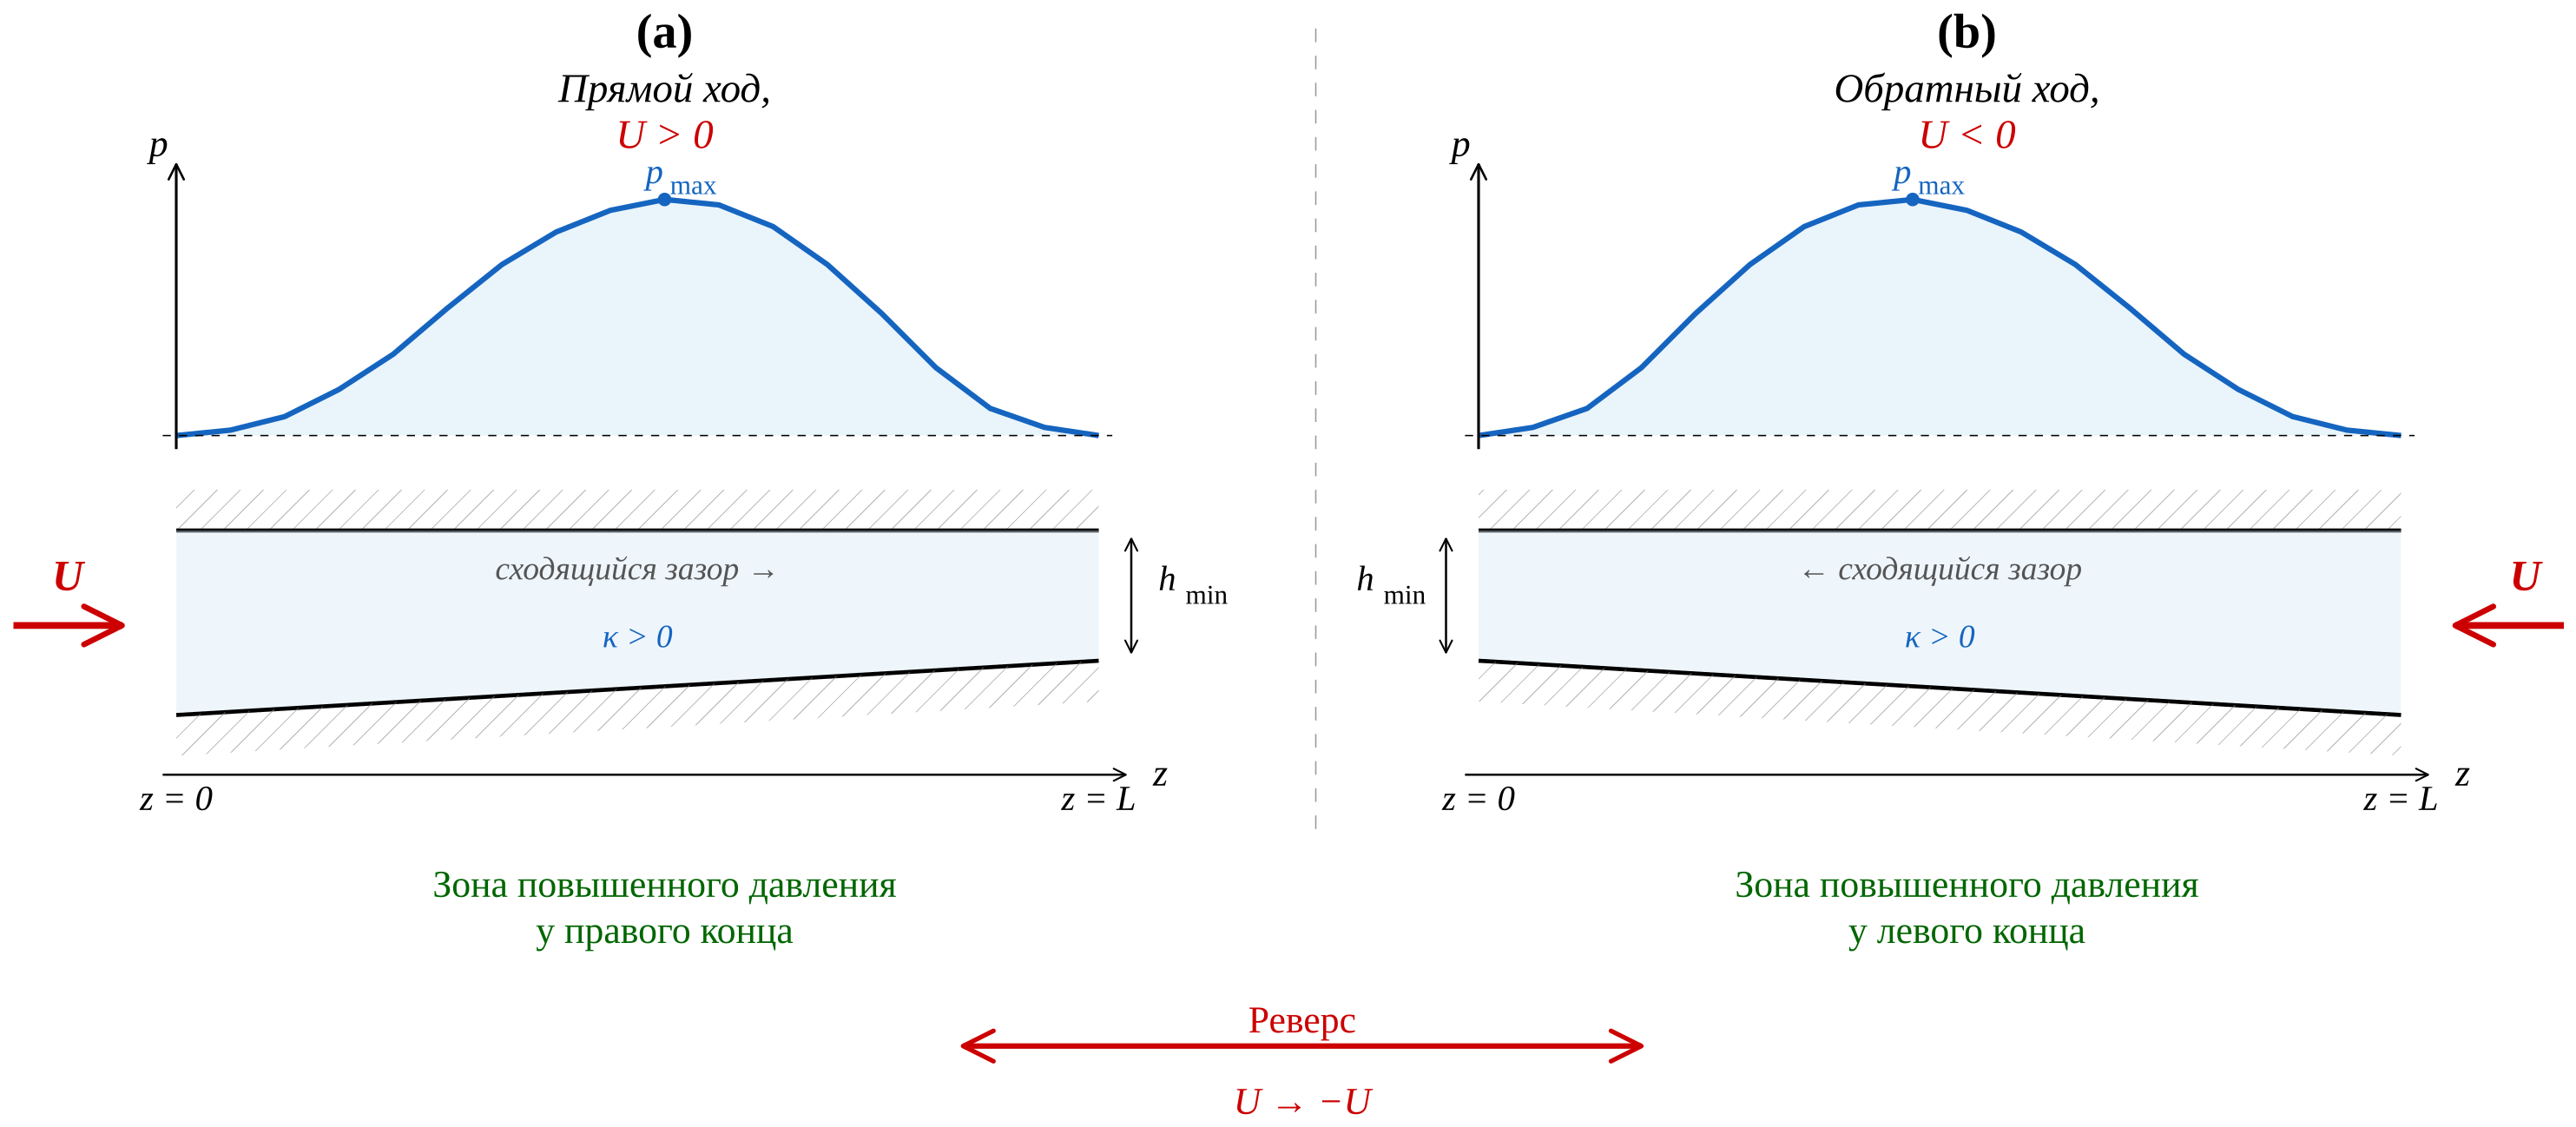
\includegraphics[width=\textwidth,height=0.9\textheight,keepaspectratio]{figures/ch02/fig_2_9.png}
\caption{Смена направления скорости $U(t)$ приводит к перемещению зоны повышенного давления: (a)~прямой ход ($U>0$); (b)~обратный ход ($U<0$). Клин вдоль~$z$ обусловлен конусностью~$\kappa$}
\label{fig:recip_reversal}
\end{figure}

\FloatBarrier

Второй член $12\mu\,\partial h/\partial t$ описывает squeeze-эффект (эффект выжимания): давление генерируется при сближении поверхностей ($\partial h/\partial t < 0$), даже если клиновой зазор вдоль $z$ отсутствует. Этот механизм важен при колебаниях эксцентриситета, вибрациях и перекосе плунжера. При удалении поверхностей ($\partial h/\partial t > 0$) данный член стремится понизить давление, что способствует возникновению кавитации.

По структуре уравнение~\eqref{eq:recip_reynolds_num} аналогично уравнениям для упорного~\eqref{eq:thrust_reynolds_num} и радиального~\eqref{eq:journal_reynolds_num} подшипников: левая часть содержит эллиптический оператор $\nabla \cdot (h^3 \nabla p)$, а правая -- источниковые члены. Отличие состоит в направлении увлечения (осевое вместо окружного) и в явной нестационарности правой части.


\subsubsection*{Граничные условия}

\textit{По окружной координате~$\theta$.} Область по~$\theta$ охватывает полную окружность, поэтому естественным условием является периодичность:
\begin{equation}
p(0, z, t) = p(2\pi, z, t), \quad
\frac{\partial p}{\partial\theta}\bigg|_{\theta=0}
= \frac{\partial p}{\partial\theta}\bigg|_{\theta=2\pi}.
\label{eq:recip_bc_periodic}
\end{equation}

\textit{По осевой координате~$z$.} Рассматриваются три варианта.

\textit{(a) Открытые торцы (атмосферные кромки, базовый вариант):}
\begin{equation}
p(\theta, 0, t) = 0, \quad p(\theta, L, t) = 0.
\label{eq:recip_bc_open}
\end{equation}

Давление отсчитывается от атмосферного ($p = p_{\mathrm{abs}} - p_{\mathrm{atm}}$), как и в подразделах~2.1.2-2.1.3. Данный вариант соответствует свободным кромкам втулки, открытым в окружающую среду.

\textit{(b) Давление подачи/слива (гидросистема):}
\begin{equation}
p(\theta, 0, t) = p_{\mathrm{in}}(t), \quad p(\theta, L, t) = p_{\mathrm{out}}(t).
\label{eq:recip_bc_pressure}
\end{equation}

Такая постановка типична для гидроцилиндров, где полости с обеих сторон поршня находятся под рабочим давлением.

\textit{(c) Уплотнённые торцы (отсутствие протекания):}
\begin{equation}
\frac{\partial p}{\partial z}\bigg|_{z=0} = 0, \quad
\frac{\partial p}{\partial z}\bigg|_{z=L} = 0.
\label{eq:recip_bc_sealed}
\end{equation}

Условие непротекания $q_z = 0$ на торцах эквивалентно $\partial p/\partial z = 0$ и применяется при наличии уплотнительных элементов на кромках втулки.

\textit{Кавитация.} При реверсе скорости и в расходящихся участках зазора давление стремится стать отрицательным. Простое ограничение $p \geq 0$ (условие Гюмбеля) нарушает баланс массы на границе кавитационной зоны. Корректный массо-сохраняющий учёт кавитации обеспечивается моделью JFO, вводимой в разделе~2.3.


\subsubsection*{Объёмные расходы}

Удельные потоки (расходы на единицу длины) определяются путём интегрирования профилей скорости по толщине смазочного слоя, аналогично подразделам~2.1.2-2.1.3.

Осевой расход (на единицу длины по окружной координате):
\begin{equation}
q_z(\theta, z, t) = \frac{h\,U(t)}{2}
  - \frac{h^3}{12\mu}\frac{\partial p}{\partial z}.
\label{eq:recip_q_z}
\end{equation}

Первое слагаемое представляет куэттовскую составляющую, обусловленную движением плунжера; второе -- пуазейлевскую составляющую, определяемую осевым градиентом давления.

Окружной расход (на единицу длины по осевой координате):
\begin{equation}
q_\theta(\theta, z, t) = -\frac{h^3}{12\mu R}\frac{\partial p}{\partial\theta}.
\label{eq:recip_q_theta}
\end{equation}

Поскольку окружные скорости обеих поверхностей равны нулю (плунжер совершает только поступательное движение), куэттовская составляющая в окружном направлении отсутствует. Окружной расход полностью определяется градиентом давления.

Полная утечка через торцы рабочей зоны:
\begin{equation}
\label{eq:recip_Q_leakage}
\begin{split}
&Q_{\mathrm{out}}(t) = \int_0^{2\pi} q_z(\theta,\,L,\,t)\,R\,\mathrm{d}\theta, \\
&Q_{\mathrm{in}}(t) = \int_0^{2\pi} q_z(\theta,\,0,\,t)\,R\,\mathrm{d}\theta.
\end{split}
\end{equation}

Знаки определяются направлением внешней нормали, как и в подразделах~2.1.2-2.1.3: положительный $Q_{\mathrm{out}}$ соответствует вытеканию смазки из рабочей зоны через торец $z = L$.

Решение уравнения Рейнольдса даёт поле давления $p(\theta, z, t)$. По найденному давлению вычисляются интегральные характеристики узла: несущая способность, расходы смазки, силы и моменты трения, минимальная толщина плёнки. Унифицированные формулы для всех выходных величин приведены в подразделе~2.1.7.

Для возвратно-поступательных узлов микротекстурирование поверхностей рассматривается как способ повышения несущей способности и снижения утечек; параметризация микрорельефа вводится в разделе~2.2.

\FloatBarrier
\subsection{Область применимости модели}

Допущения, положенные в основу уравнения Рейнольдса, перечислены в подразделе~2.1.1 (п.~1-8). Ниже для каждого из них указаны условия, при которых допущение может нарушаться, и соответствующие расширения модели. Часть расширений реализована в последующих разделах и главах настоящей работы.

\subsubsection*{Геометрия тонкого слоя}

Смазочная аппроксимация предполагает малость отношения $\epsilon = H/L \ll 1$, где $H$ -- характерная толщина смазочного слоя (подраздел~2.1.1), и малые уклоны поверхностей $|\partial h/\partial x| \ll 1$, $|\partial h/\partial z| \ll 1$. При широких зазорах, очень коротких контактах или наличии резких кромок и ступенек эти условия нарушаются, и необходимо обращаться к CFD-моделированию на основе полных уравнений Навье--Стокса. Локальные большие уклоны, связанные с микроструктурами (раздел~2.2), формально выходят за рамки классической смазочной аппроксимации. На практике применение уравнения Рейнольдса остаётся корректным, если глубина микроструктуры $h_p$ мала по сравнению с зазором ($h_p / h_0 \ll 1$), а длина переходного участка $\ell_p$ обеспечивает малость уклона: $|\partial h/\partial x| \sim h_p/\ell_p \ll 1$.

\subsubsection*{Инерция}

Инерционные члены пренебрежимо малы при $\mathrm{Re}\,\epsilon \ll 1$, см.~\eqref{eq:Re_epsilon}. При высоких скоростях, низкой вязкости или увеличенном зазоре этот параметр растёт, и инерционные эффекты становятся существенными. В таких случаях применяются инерционные поправки к уравнению Рейнольдса или переход к полным уравнениям Навье--Стокса. В типичных режимах подшипников скольжения, рассматриваемых в настоящей работе, малость зазора ($\epsilon \ll 1$) и умеренные скорости обеспечивают $\mathrm{Re}\,\epsilon \ll 1$.

\subsubsection*{Ламинарность}

С ростом скорости и зазора или при снижении вязкости течение может утратить устойчивость и перейти в турбулентный режим. В турбулентном режиме обычно модифицируют расходные соотношения, вводя эффективные коэффициенты потока, что приводит к <<турбулентному>> уравнению Рейнольдса (подходы Hirs, Ng--Pan). В настоящей работе рассматривается ламинарный режим, характерный для подшипников скольжения при малых зазорах.

\subsubsection*{Несжимаемость}

При газовой смазке или при высоких давлениях, вызывающих заметное изменение плотности, допущение $\rho = \mathrm{const}$ нарушается. Сжимаемая форма уравнения Рейнольдса записывается через баланс массы:
\begin{equation}
\frac{\partial (\rho h)}{\partial t}
+ \frac{\partial (\rho\, q_x)}{\partial x}
+ \frac{\partial (\rho\, q_z)}{\partial z} = 0,
\label{eq:reynolds_compressible}
\end{equation}
где $q_x$ и $q_z$ -- удельные расходы~\eqref{eq:flow_rate_x},~\eqref{eq:flow_rate_z}. При $\rho = \mathrm{const}$ уравнение~\eqref{eq:reynolds_compressible} сводится к уже полученному уравнению~\eqref{eq:reynolds_full}. Для жидких смазочных материалов при умеренных давлениях плотность практически постоянна. В настоящей работе рассматривается несжимаемая жидкость.

\subsubsection*{Постоянная вязкость и изотермичность}

Интенсивный сдвиг в тонкой смазочной плёнке может приводить к значительному вязкостному нагреву. В этом случае вязкость становится функцией температуры, $\mu = \mu(T)$, и уравнение Рейнольдса необходимо решать совместно с уравнением энергии -- термогидродинамическая (THD) постановка. При высоких контактных давлениях существенной становится пьезовязкость $\mu = \mu(p)$, характерная для упругогидродинамической смазки (EHL). В обобщённом уравнении Рейнольдса~\eqref{eq:reynolds_full} вязкость записана под знаком производных, что обеспечивает корректность формулы и при переменной вязкости $\mu = \mu(x, z)$. Влияние температурной зависимости вязкости рассматривается в главе~4.

\subsubsection*{Условие прилипания}

При очень малых зазорах (порядка десятков нанометров) или при наличии специальных покрытий (гидрофобных, олеофобных) возможно проскальзывание жидкости на стенке (Navier slip). В данной работе скольжение на границе не учитывается.

\subsubsection*{Жёсткие поверхности}

Модель предполагает геометрически заданный зазор $h(x, z, t)$, не зависящий от давления. При высоких нагрузках или использовании податливых материалов упругая деформация поверхностей изменяет форму зазора, что приводит к упругогидродинамической (EHL) постановке: уравнение Рейнольдса решается совместно с уравнением упругости. В настоящей работе поверхности полагаются жёсткими.

\subsubsection*{Кавитация}

В областях расходящегося зазора давление, полученное из уравнения Рейнольдса, может становиться отрицательным, что физически соответствует разрыву сплошности смазочного слоя (кавитации). Простое ограничение $p \geq 0$ (условие Гюмбеля) нарушает баланс массы на границе кавитационной зоны. Массо-сохраняющий подход Jakobsson--Floberg--Olsson (JFO), обеспечивающий корректное описание кавитации, вводится в разделе~2.3.

В рамках настоящей работы базовые допущения расширяются в следующих направлениях:
\begin{itemize}
  \item кавитация и массо-сохранение -- раздел~2.3;
  \item микроструктуры поверхности -- раздел~2.2;
  \item температурная зависимость вязкости $\mu(T)$ -- глава~4.
\end{itemize}
Упругие деформации поверхностей (EHL), турбулентность, сжимаемость и скольжение на границе в рамках настоящей работы не рассматриваются.

Допущения модели Рейнольдса, условия их нарушения и возможные
расширения систематизированы
в таблице~\ref{tab:model_limits}.

\begin{table}[!ht]
\centering
\caption{Допущения модели Рейнольдса, условия их применимости
  и возможные расширения}
\label{tab:model_limits}
\begin{tabularx}{\textwidth}{|X|X|X|}
\hline
\multicolumn{1}{|c|}{\textbf{Допущение}}
  & \multicolumn{1}{c|}{\textbf{Когда нарушается}}
  & \multicolumn{1}{c|}{\textbf{Расширение модели}} \\
\hline
Изотермическая смазка ($T = T_0$, $\mu = \mathrm{const}$)
  & Высокие нагрузки и скорости, интенсивная вязкостная
    диссипация
  & THD-постановка (уравнение энергии) \\
\hline
Ньютоновская смазка
  & Добавки к смазке, высокие скорости сдвига
    ($\dot\gamma > 10^5$~с$^{-1}$)
  & Модели Карро, Эйри и~др. \\
\hline
Несжимаемость ($\rho = \mathrm{const}$)
  & Давление порядка $0{,}5$~ГПа и выше (EHL-режим)
  & Уравнение Тейта для $\rho(p)$ \\
\hline
Постоянная вязкость
  & Пьезовязкостные смазки, давление выше $0{,}1$~ГПа
  & Уравнение Баруса $\mu = \mu_0 e^{\alpha p}$ \\
\hline
Гладкие поверхности
  & Смешанный/граничный режим ($\lambda_r = h/\sigma < 3$)
  & Осреднённое уравнение Патира--Ченга \\
\hline
Ламинарное течение
  & Число Рейнольдса плёнки $Re_f > 1$
    ($Re_f = \rho U h / \mu$)
  & Турбулентные поправки \\
\hline
\end{tabularx}
\end{table}

\FloatBarrier

Принятые допущения соответствуют классической
гидродинамической теории смазки Рейнольдса и обоснованы для
жидкостного и смешанного режимов при умеренных давлениях
($p < 50$~МПа) и скоростях ($Re_f < 1$). По сравнению
с прямым CFD-моделированием тонкого смазочного слоя (решение
уравнений Навье--Стокса в трёхмерной постановке) уравнение
Рейнольдса на несколько порядков дешевле при сопоставимой
точности в зоне своей применимости. Это принципиально важно
для параметрических расчётов, оптимизации геометрии
микроструктур и анализа динамических коэффициентов, где
требуется многократное решение задачи~\cite{hori2002,suddapalli2015}.

\FloatBarrier
\subsection{Безразмерная постановка}

Переход к безразмерным переменным унифицирует три частные постановки, сформулированные в подразделах~2.1.2-2.1.4, и позволяет сравнивать различные конфигурации подшипников и режимы их работы на единой шкале. Кроме того, безразмеризация сокращает число определяющих параметров задачи до нескольких безразмерных групп, что упрощает параметрический анализ. Введённый аппарат используется далее при исследовании влияния микроструктур поверхности (раздел~2.2) и при численной дискретизации (глава~3).

\subsubsection*{Характерные масштабы и безразмерные переменные}

Общая схема масштабирования повторяет подход, применённый при выводе уравнения Рейнольдса в подразделе~2.1.1~\cite{hori2002,szeri1998}, но теперь записывается в обобщённых обозначениях, пригодных для всех трёх постановок:
%
\begin{equation}
\bar{s}_1 = \frac{s_1}{L_1}, \quad
\bar{s}_2 = \frac{s_2}{L_2}, \quad
\bar{h}   = \frac{h}{h_0},   \quad
\bar{p}   = \frac{p}{p_0},   \quad
\bar{U}   = \frac{U}{U_0},   \quad
\bar{t}   = \frac{t}{t_0},
\label{eq:nondim_vars}
\end{equation}
%
\begin{conditions}
$s_1$, $s_2$ -- поверхностные координаты (конкретные для каждой постановки, см.\ таблицу~\ref{tab:nondim_scales} ниже);\\
$h_0$ -- характерная толщина зазора (радиальный зазор $c$ или средний зазор);\\
$U_0$ -- характерная скорость увлечения;\\
$t_0$ -- характерное время (для нестационарных задач).
\end{conditions}
Масштаб давления выбирается так, чтобы клиновой член в правой части уравнения Рейнольдса имел порядок единицы. Из баланса~\eqref{eq:pressure_scale} следует:
%
\begin{equation}
p_0 = \frac{6\,\mu_0\,U_0\,L_1}{h_0^2},
\label{eq:nondim_p0}
\end{equation}
%
\begin{conditions}
$L_1$ -- масштаб длины вдоль направления увлечения (координата $s_1$);\\
$\mu_0$ -- характерное значение вязкости.
\end{conditions}

\subsubsection*{Безразмерное уравнение Рейнольдса}

Подставляя масштабы~\eqref{eq:nondim_vars},~\eqref{eq:nondim_p0} в обобщённое уравнение Рейнольдса~\eqref{eq:reynolds_full} и сокращая размерные множители, получаем единую безразмерную форму:
%
\begin{equation}
\frac{\partial}{\partial \bar{s}_1}\!\left(\bar{h}^{\,3}\,\frac{\partial \bar{p}}{\partial \bar{s}_1}\right)
+ \Lambda^2\,\frac{\partial}{\partial \bar{s}_2}\!\left(\bar{h}^{\,3}\,\frac{\partial \bar{p}}{\partial \bar{s}_2}\right)
= \bar{U}\,\frac{\partial \bar{h}}{\partial \bar{s}_1}
+ \sigma\,\frac{\partial \bar{h}}{\partial \bar{t}},
\label{eq:reynolds_nondim}
\end{equation}
%
где введены две безразмерные группы:
%
\begin{equation}
\Lambda = \frac{L_1}{L_2}
\label{eq:nondim_Lambda}
\end{equation}
%
-- параметр удлинённости (aspect ratio), характеризующий соотношение продольного и поперечного масштабов, и
%
\begin{equation}
\sigma = \frac{2\,L_1}{U_0\,t_0}
\label{eq:nondim_sigma}
\end{equation}
%
-- параметр нестационарности (squeeze number), определяющий относительный вклад выжимания плёнки.

При $\sigma = 0$ (либо в стационарной задаче) член выжимания отсутствует, и уравнение содержит только клиновой источник. Параметр $\Lambda$ определяет относительный вклад поперечного растекания: при $\Lambda \ll 1$ вклад второго члена мал и задача приближается к одномерной по $s_1$; при $\Lambda \gg 1$ доминирует поперечное растекание по $s_2$, что соответствует <<короткому>> приближению в терминологии радиального подшипника (подраздел~2.1.3). Для цилиндрических координат, используемых в постановках~2.1.2-2.1.4, в левой части уравнения~\eqref{eq:reynolds_nondim} появляются дополнительные множители $1/\bar{r}$ и $1/\bar{r}^{\,2}$, однако общая структура уравнения сохраняется.

\subsubsection*{Масштабы для частных постановок}

Конкретные значения масштабов для трёх постановок, рассмотренных в подразделах~2.1.2-2.1.4, приведены в таблице~\ref{tab:nondim_scales}.

\begin{table}[!ht]
\centering
\caption{Характерные масштабы для безразмерной постановки}
\label{tab:nondim_scales}
\resizebox{\textwidth}{!}{%
\begin{tabular}{|l|c|c|c|c|c|c|c|c|}
\hline
\multicolumn{1}{|c|}{\textbf{Постановка}} & $\boldsymbol{s_1}$ & $\boldsymbol{s_2}$ & $\boldsymbol{L_1}$ & $\boldsymbol{L_2}$ & $\boldsymbol{h_0}$ & $\boldsymbol{U_0}$ & $\boldsymbol{p_0}$ & $\boldsymbol{t_0}$ \\
\hline
Упорная (2.1.2)
  & $R\theta$ & $r$ & $R$ & $R_{\mathrm{out}} - R_{\mathrm{in}}$
  & $h_{\min}$ или $h_{\mathrm{mean}}$
  & $\omega R$ & $\dfrac{6\mu_0\omega R^2}{h_0^2}$ & --
\\[6pt]
\hline
Радиальная (2.1.3)
  & $R\theta$ & $z$ & $R$ & $L$
  & $c$
  & $\omega R$ & $\dfrac{6\mu_0\omega R^2}{c^2}$ & --
\\[6pt]
\hline
Возвратно-пост.\ (2.1.4)
  & $z$ & $R\theta$ & $L$ & $R$
  & $c$
  & $\max|U(t)|$ & $\dfrac{6\mu_0\,U_0\,L}{c^2}$ & $1/\Omega$
\\[6pt]
\hline
\end{tabular}%
}
\end{table}

\FloatBarrier

В упорной и радиальной постановках задача стационарна, поэтому временной масштаб $t_0$ не требуется (обозначено <<-->>{} в таблице). Координата $s_1$ соответствует направлению увлечения, а $s_2$ -- поперечному направлению. Для упорного подшипника $R$ -- характерный радиус (например, $R_{\mathrm{out}}$ или среднее значение $(R_{\mathrm{in}} + R_{\mathrm{out}})/2$). При подстановке масштабов из таблицы в общее уравнение~\eqref{eq:reynolds_nondim} получаются безразмерные формы, согласованные с размерными уравнениями~\eqref{eq:thrust_reynolds_num},~\eqref{eq:journal_reynolds_num},~\eqref{eq:recip_reynolds_num}.

Характерный масштаб давления~$p_0 = 6\mu_0 U_0 L_1 / h_0^2$
(формула~\eqref{eq:nondim_p0}) определяет, при каких реальных
давлениях безразмерное поле~$P$ имеет порядок единицы.
Для радиального подшипника насоса (глава~5): $\mu_0 = 0{,}01105$~Па$\cdot$с,
$U_0 = \omega R = 10{,}9$~м/с, $L_1 = R = 0{,}035$~м,
$h_0 = c = 50$~мкм:
%
\begin{equation}
  p_0 = \frac{6 \cdot 0{,}01105 \cdot 10{,}9
    \cdot 0{,}035}{(50 \cdot 10^{-6})^2}
  \approx 10{,}1 \;\text{МПа}.
  \label{eq:p0_example}
\end{equation}
%
Максимальные безразмерные давления в расчётах глав 5--6 имеют
порядок $10^{-1}$, что соответствует размерным значениям
порядка единиц мегапаскалей,~-- в пределах применимости
изотермической постановки. Для упорного подшипника (глава~7)
масштаб~$p_0$ иной вследствие меньшего характерного зазора
и другой скорости, что объясняет различие в абсолютных
значениях несущей способности при схожих безразмерных уровнях
давления.

Параметр $\Lambda = L_1/L_2$~\eqref{eq:nondim_Lambda}
физически характеризует соотношение «продольного»
и «поперечного» масштабов задачи вдоль направления увлечения
и поперёк него (таблица~\ref{tab:nondim_scales}).
Для радиального подшипника $L_1 = R$, $L_2 = L$ (длина
подшипника), поэтому $\Lambda = R/L$. При малых $\Lambda$
($R \ll L$, узкий и длинный подшипник) поперечным растеканием
можно пренебречь, и задача сводится к одномерной по~$s_1$~--
это «бесконечно длинное» приближение. При больших $\Lambda$
($R \gg L$, широкий и короткий подшипник) давление быстро
выравнивается по~$s_1$, и поперечный градиент определяет
структуру течения~-- это «короткое» приближение. Для реальных
подшипников $L/D \approx 0{,}5$--$1{,}5$, откуда
$\Lambda \approx 0{,}33$--$1{,}0$, что соответствует
промежуточному режиму с существенным вкладом обоих членов
в уравнении~\eqref{eq:reynolds_nondim}.

Введённые масштабы определяют безразмерную форму уравнения Рейнольдса и базовой геометрии зазора. Параметры, характеризующие микроструктуры поверхности, -- безразмерная глубина $h_p/h_0$, размеры элементов, плотность покрытия -- вводятся отдельно в подразделе~2.2.4. Далее в работе, если не оговорено иное, используются безразмерные переменные; черта над символом опускается для краткости записи.

\FloatBarrier
\subsection{Целевые функционалы и выходные величины}

Решение уравнения Рейнольдса даёт поле давления $p(s_1, s_2, t)$
в смазочном слое. По найденному давлению и известной геометрии
зазора $h(s_1, s_2, t)$ вычисляются интегральные характеристики узла,
определяющие его работоспособность и энергоэффективность.
В настоящем подразделе приведены унифицированные формулы
для всех трёх постановок (2.1.2-2.1.4).

Элемент площади $dA$ для каждой постановки:
\begin{itemize}
  \item упорная (2.1.2): $dA = r\,dr\,d\theta$,\quad
        $r \in [R_{\mathrm{in}},\,R_{\mathrm{out}}]$,\;
        $\theta \in [0,\,2\pi]$;
  \item радиальная (2.1.3): $dA = R\,d\theta\,dz$,\quad
        $\theta \in [0,\,2\pi]$,\; $z \in [0,\,L]$;
  \item возвратно-поступательная (2.1.4): $dA\!=\!R\,d\theta\,dz$,\,
        $\theta\!\in\![0,\,2\pi]$,\, $z\!\in\![0,\,L]$.
\end{itemize}

%% ===== Блок 1: Несущая способность =====
\subsubsection*{Несущая способность}

Для упорного подшипника результирующая нагрузка направлена вдоль оси
вращения и является скалярной величиной:
\begin{equation}
  W = \iint_A p\,dA
    = \int_0^{2\pi}\!\int_{R_{\mathrm{in}}}^{R_{\mathrm{out}}}
      p(r,\theta)\,r\,dr\,d\theta.
  \label{eq:func_W_thrust}
\end{equation}

Для радиального и возвратно-поступательного подшипников давление
распределено по цилиндрической поверхности, поэтому результирующая
сила имеет две компоненты в плоскости поперечного сечения.
Нормаль к поверхности вала направлена радиально наружу:
$\mathbf{n} = (\cos\theta,\,\sin\theta)$.
Гидродинамическая сила, действующая на вал со стороны смазочного слоя,
определяется как:
Поскольку давление действует на поверхность вала по направлению
внутрь ($d\mathbf{F} = -p\,\mathbf{n}\,dA$), компоненты силы
содержат знак <<минус>>:
\begin{equation}
\begin{alignedat}{2}
  & F_x(t) &\;=\;& -\int_0^L \int_0^{2\pi}
    p(\theta,z,t)\,\cos\theta\;R\,d\theta\,dz, \\
  & F_y(t) &\;=\;& -\int_0^L \int_0^{2\pi}
    p(\theta,z,t)\,\sin\theta\;R\,d\theta\,dz, \\
  & F(t)   &\;=\;& \sqrt{F_x^2(t) + F_y^2(t)}.
\end{alignedat}
  \label{eq:func_F_components}
\end{equation}
Здесь ось $x$ соответствует направлению $\theta = 0$,
ось $y$ -- направлению $\theta = \pi/2$.
Угол нагружения (attitude angle):
\begin{equation}
  \psi(t) = \mathrm{atan2}\bigl(F_y(t),\,F_x(t)\bigr).
  \label{eq:func_psi}
\end{equation}

Угол $\psi$ определяет направление результирующей гидродинамической
силы относительно оси $x$ и используется при анализе орбит вала
(главы~5-8).
Для стационарного радиального подшипника зависимость от $t$ отсутствует.
Схема компонент силы показана на рис.~\ref{fig:force_components}.

% [РИСУНОК: Компоненты гидродинамической силы]
\begin{figure}[!ht]
\centering
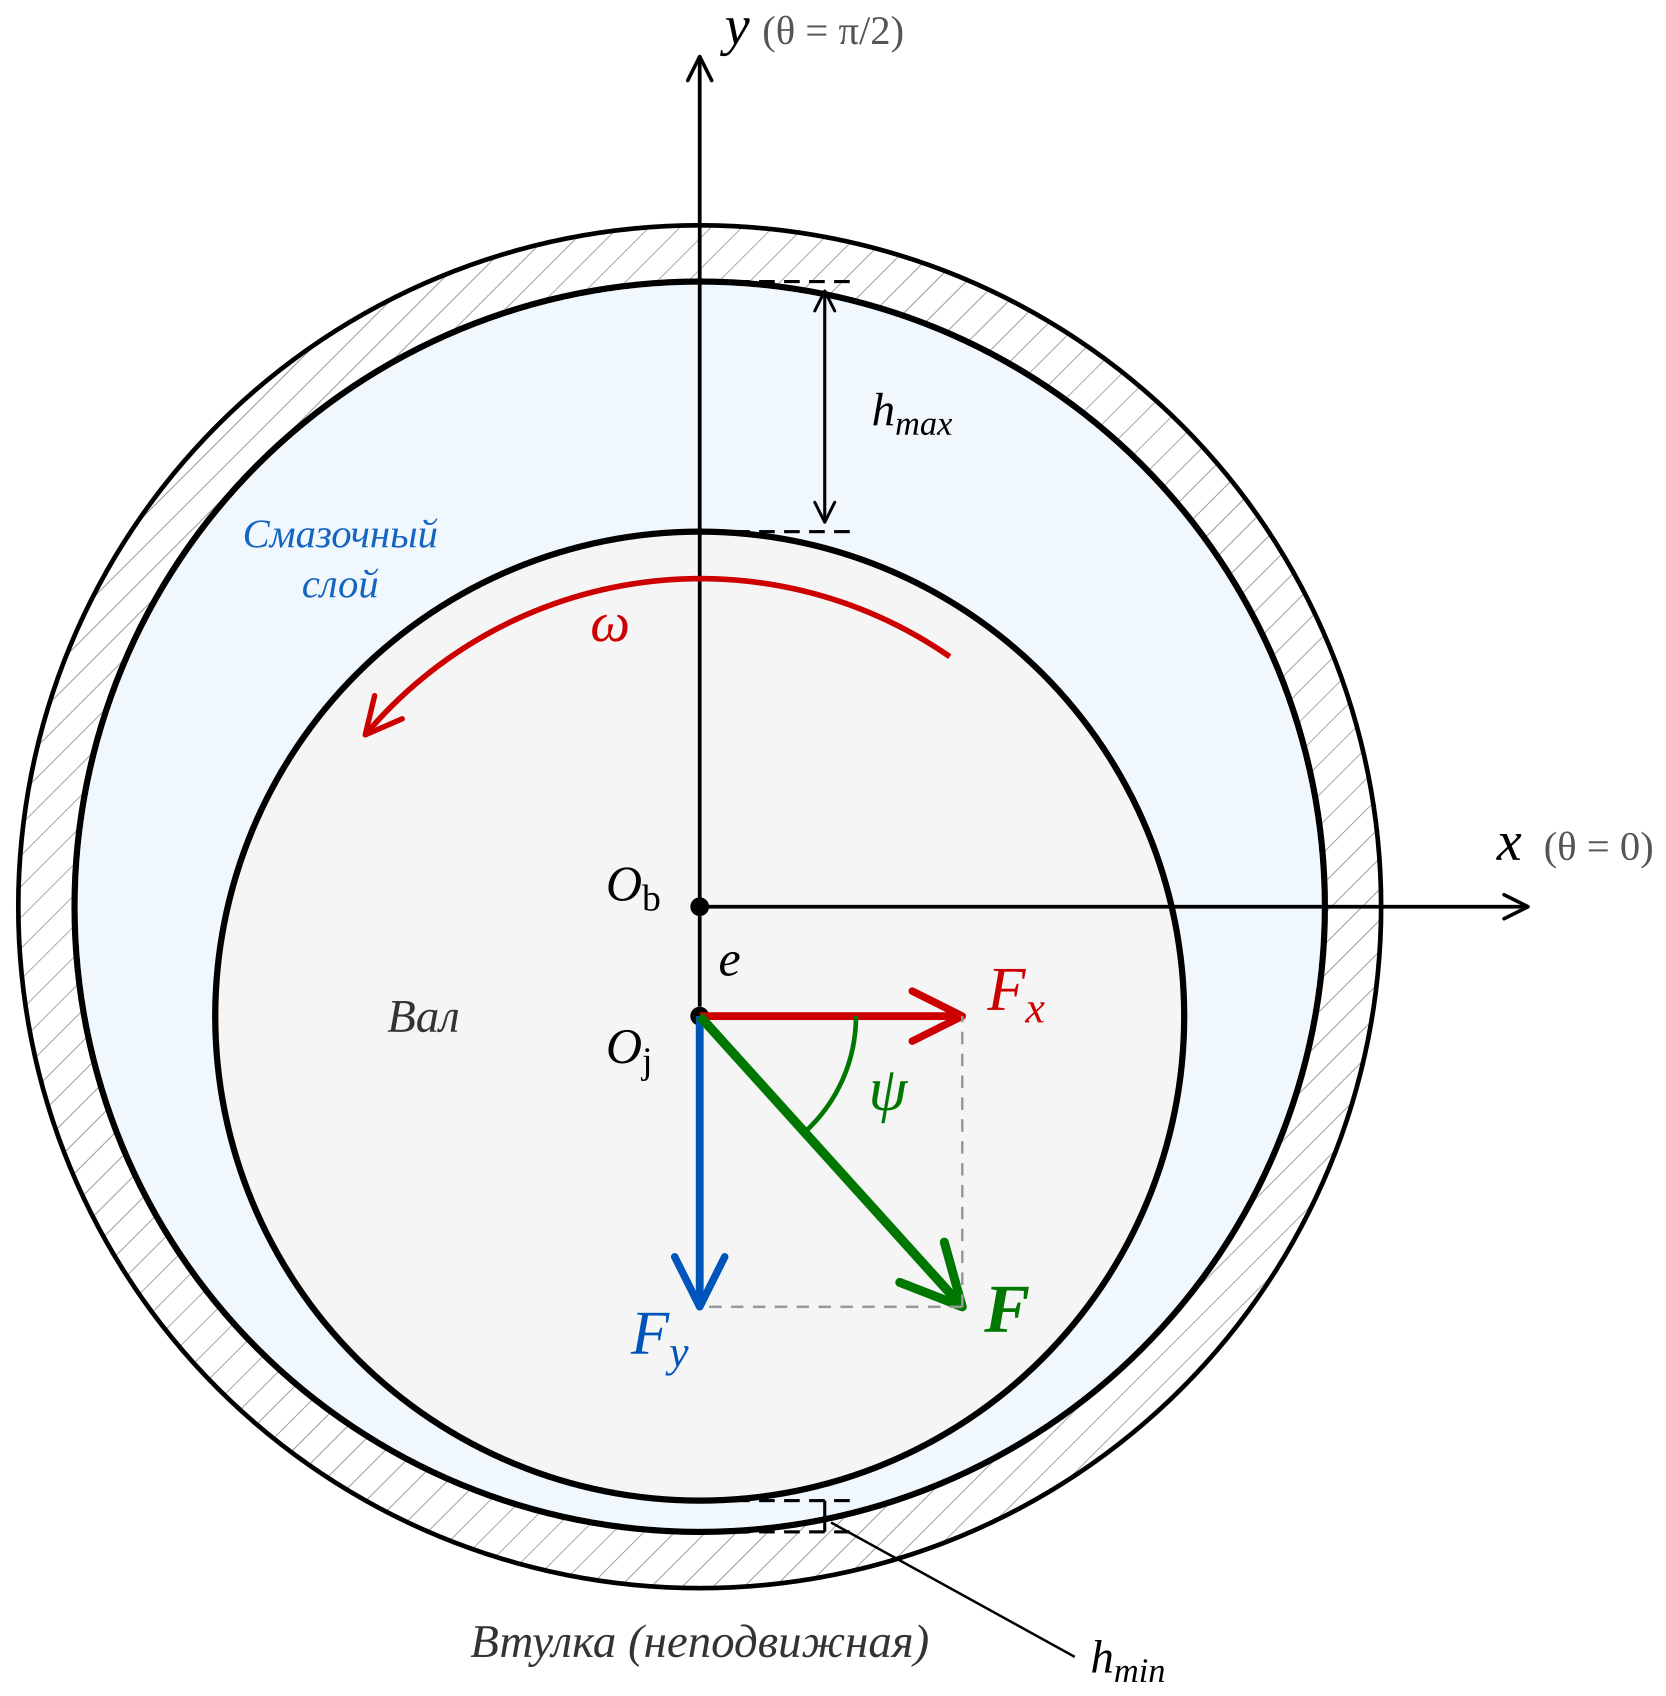
\includegraphics[width=\textwidth,height=0.9\textheight,keepaspectratio]{figures/ch02/fig_2_10.png}
\caption{Компоненты гидродинамической силы на валу/плунжере}
\label{fig:force_components}
\end{figure}

%% ===== Блок 2: Расходы и утечки =====
\subsubsection*{Расходы и утечки}

Удельные потоки $q$ определены в соответствующих постановках
(см.~\eqref{eq:thrust_q_r}, \eqref{eq:journal_q_z},
\eqref{eq:recip_q_z}).
Здесь приводятся только интегральные расходы через границы
рабочей зоны.

Упорный подшипник -- суммарные объёмные расходы через наружную
и внутреннюю кромки (см.~также~\eqref{eq:thrust_Q_radial}):
\begin{equation}
\label{eq:func_Q_thrust}
\begin{split}
  &Q_{\mathrm{out}} = \int_0^{2\pi}
    q_r(R_{\mathrm{out}},\theta)\,R_{\mathrm{out}}\,d\theta, \\
  &Q_{\mathrm{in}} = \int_0^{2\pi}
    q_r(R_{\mathrm{in}},\theta)\,R_{\mathrm{in}}\,d\theta.
\end{split}
\end{equation}

Радиальный подшипник -- утечки через торцы
(см.~также~\eqref{eq:journal_Q_side}):
\begin{equation}
  Q_{\mathrm{out}} = \int_0^{2\pi}
    q_z(\theta,L)\,R\,d\theta,
  \quad
  Q_{\mathrm{in}} = \int_0^{2\pi}
    q_z(\theta,0)\,R\,d\theta.
  \label{eq:func_Q_journal}
\end{equation}

Возвратно-поступательный подшипник -- мгновенные расходы через
обе границы и их усреднение по периоду
(см.~также~\eqref{eq:recip_Q_leakage}):
\begin{equation}
  Q_{\mathrm{out}}(t) = \int_0^{2\pi}
    q_z(\theta,L,t)\,R\,d\theta,
  \quad
  Q_{\mathrm{in}}(t) = \int_0^{2\pi}
    q_z(\theta,0,t)\,R\,d\theta,
  \label{eq:func_Q_recip}
\end{equation}
\begin{equation}
  \langle Q_{\mathrm{out}} \rangle
    = \frac{1}{T}\int_0^T Q_{\mathrm{out}}(t)\,dt,
  \quad
  \langle Q_{\mathrm{in}} \rangle
    = \frac{1}{T}\int_0^T Q_{\mathrm{in}}(t)\,dt,
  \label{eq:func_Q_recip_avg}
\end{equation}
где $T = 2\pi/\Omega$ -- период возвратно-поступательного движения.

Положительный $Q_{\mathrm{out}}$ соответствует вытеканию смазки
из рабочей зоны, что согласуется с конвенцией, принятой
в подразделах~2.1.2-2.1.4.

%% ===== Блок 3: Трение, момент трения, потери мощности =====
\subsubsection*{Сила и момент трения}

Касательное напряжение вдоль направления увлечения $s_1$
следует из профиля скорости~\eqref{eq:velocity_profile_u}.
Первое слагаемое -- вязкое (куэттовское), второе -- давленческое
(пуазейлевское).
Выражения для касательного напряжения на подвижной ($y = h$)
и неподвижной ($y = 0$) поверхностях:
\begin{equation}
  \tau\big|_{y=h} = \frac{\mu\,U}{h}
    + \frac{h}{2}\,\frac{\partial p}{\partial s_1},
  \quad
  \tau\big|_{y=0} = \frac{\mu\,U}{h}
    - \frac{h}{2}\,\frac{\partial p}{\partial s_1}.
  \label{eq:func_tau_both}
\end{equation}

Далее при вычислении момента и силы трения используется напряжение
на неподвижной поверхности $\tau|_{y=0}$, что даёт силу сопротивления
движению.

Конкретизация производной $\partial p/\partial s_1$ и скорости $U$
для каждой постановки:
\begin{itemize}
  \item радиальная: $s_1 = R\theta$ $\Rightarrow$
        $\partial p/\partial s_1 = (1/R)\,\partial p/\partial\theta$,\;
        $U = \omega R$;
  \item упорная: $s_1 = r\theta$ $\Rightarrow$
        $\partial p/\partial s_1 = (1/r)\,\partial p/\partial\theta$,\;
        $U = \omega r$;
  \item возвратно-поступательная: $s_1 = z$ $\Rightarrow$
        $\partial p/\partial s_1 = \partial p/\partial z$,\;
        $U = U(t)$.
\end{itemize}

В приведённых ниже интегралах $\tau$ обозначает касательное
напряжение на неподвижной поверхности $\tau|_{y=0}$.

Момент трения для упорного подшипника:
\begin{equation}
  M_f = \int_0^{2\pi}\!\int_{R_{\mathrm{in}}}^{R_{\mathrm{out}}}
    \tau(r,\theta)\,r^2\,dr\,d\theta.
  \label{eq:func_Mf_thrust}
\end{equation}

Момент трения для радиального подшипника:
\begin{equation}
  M_f = \int_0^L\!\int_0^{2\pi}
    \tau(\theta,z)\,R^2\,d\theta\,dz.
  \label{eq:func_Mf_journal}
\end{equation}

Сила трения для возвратно-поступательного подшипника:
\begin{equation}
  F_f(t) = \int_0^L\!\int_0^{2\pi}
    \tau(\theta,z,t)\,R\,d\theta\,dz.
  \label{eq:func_Ff_recip}
\end{equation}

Потери мощности на трение для вращательных постановок:
\begin{equation}
  P_f = M_f \cdot \omega.
  \label{eq:func_Pf_rot}
\end{equation}

При принятой конвенции (касательное напряжение на неподвижной
поверхности) величины $M_f$ и $F_f$ представляют сопротивление
движению, и потери мощности $P_f \geq 0$.

Для возвратно-поступательной постановки мощность потерь является
функцией времени:
\begin{equation}
  P_f(t) = |F_f(t) \cdot U(t)|,
  \quad
  \langle P_f \rangle = \frac{1}{T}\int_0^T P_f(t)\,dt.
  \label{eq:func_Pf_recip}
\end{equation}

Модуль обеспечивает неотрицательность потерь при смене направления
скорости.

%% ===== Блок 4: Минимальная толщина плёнки =====
\subsubsection*{Минимальная толщина плёнки}

\begin{equation}
  h_{\min}(t) = \min_{(s_1,\,s_2)\,\in\,\Omega}\,h(s_1,s_2,t).
  \label{eq:func_hmin}
\end{equation}

Минимальная толщина плёнки -- критический параметр работоспособности:
при $h_{\min} \to 0$ нарушается режим жидкостного трения.
Для стационарных задач $h_{\min}$ является числом,
для нестационарных -- функцией времени.
Дополнительно может представлять интерес максимальное давление
$p_{\max}(t) = \max_\Omega p$.

%% ===== Блок 5: Коэффициент трения =====
\subsubsection*{Коэффициент трения}

Безразмерный коэффициент трения для радиального
и возвратно-поступательного узлов:
\begin{equation}
  f(t) = \frac{|F_f(t)|}{F(t)}.
  \label{eq:func_f}
\end{equation}

Для упорного подшипника естественнее определять коэффициент трения
через момент:
\begin{equation}
  f_T = \frac{M_f}{W \cdot R_m},
  \quad
  R_m = \frac{R_{\mathrm{in}} + R_{\mathrm{out}}}{2}.
  \label{eq:func_fT}
\end{equation}

%% ===== Завершающий абзац =====

Введённые функционалы определяют основные цели при анализе
и оптимизации подшипников скольжения:
\begin{itemize}
  \item максимизация несущей способности $W$ (или $F$);
  \item минимизация потерь на трение $P_f$ (или $M_f$);
  \item минимизация утечек $Q_{\mathrm{out}}$;
  \item обеспечение $h_{\min}$ выше критического порога
        (предотвращение сухого контакта)~\cite{sfyris2012,chasalevris2012,chasalevris2013}.
\end{itemize}
Для нестационарных задач (подраздел~2.1.4) анализ проводится
как для мгновенных значений, так и для усреднённых по периоду
$\langle \cdot \rangle$.


\FloatBarrier
\section{Модель с детерминированными микроструктурами}
\subsection{Параметризация микрорельефа}

В разделе~2.1 рассмотрены постановки задачи смазки для гладких
поверхностей. Для учёта детерминированных микроструктур необходимо
задать модификацию функции зазора~$h$, описывающую геометрию
нанесённых на поверхность элементов. Настоящий подраздел вводит общую
параметрическую модель микрорельефа, используемую далее
в~2.2.2-2.2.4. Формулы записываются для произвольных поверхностных
координат; конкретные координаты определяются постановкой
(таблица~\ref{tab:nondim_scales} в подразделе~2.1.6).

%% ===== Блок 1: Суперпозиция =====

\subsubsection*{Суперпозиция зазора}

Рабочую поверхность представляем в виде гладкой базовой поверхности
с наложенными регулярными элементами. Суммарная толщина смазочного
слоя записывается как суперпозиция базового зазора и добавки,
описывающей микрорельеф:
\begin{equation}
  h(x_1, x_2)
    = h_{\mathrm{base}}(x_1, x_2) + \Delta h(x_1, x_2),
  \label{eq:h_superposition}
\end{equation}
где $(x_1, x_2)$ -- поверхностные координаты с размерностью длины.
В зависимости от постановки:
\begin{itemize}
  \item радиальный подшипник: $x_1 = R\theta$, $x_2 = z$;
  \item возвратно-поступательная постановка: $x_1 = z$,
        $x_2 = R\theta$;
  \item упорный подшипник: $x_1 = R\theta$, $x_2 = r$,
\end{itemize}
где $R$ -- характерный радиус (подраздел~2.1.6). Для упорного
подшипника дуговая координата по окружному направлению в общем случае
равна $r\theta$; здесь используется аппроксимация $x_1 = R\theta$
с характерным (например, средним) радиусом, что удобно для
унифицированного задания микрорельефа и раскладки.

Слагаемые в~\eqref{eq:h_superposition} имеют следующий смысл:
\begin{itemize}
  \item $h_{\mathrm{base}}$ -- толщина зазора для гладкой поверхности,
        определённая в подразделах~2.1.2-2.1.4;
  \item $\Delta h$ -- локальная добавка, описывающая микрорельеф.
\end{itemize}
Знаковая конвенция: $\Delta h \geq 0$ для углублений (лунок),
$\Delta h \leq 0$ для выступов. Принцип суперпозиции проиллюстрирован
на рисунке~\ref{fig:h_superposition}.

% [РИСУНОК: Суперпозиция зазора h = h_base + Δh]
% Должен показывать два вида:
% (1) Продольный разрез: базовый клин h_base + ямка Δh → суммарный h
% (2) Вид сверху: пятно одного элемента микроструктуры на фоне сектора
\begin{figure}[!ht]
\centering
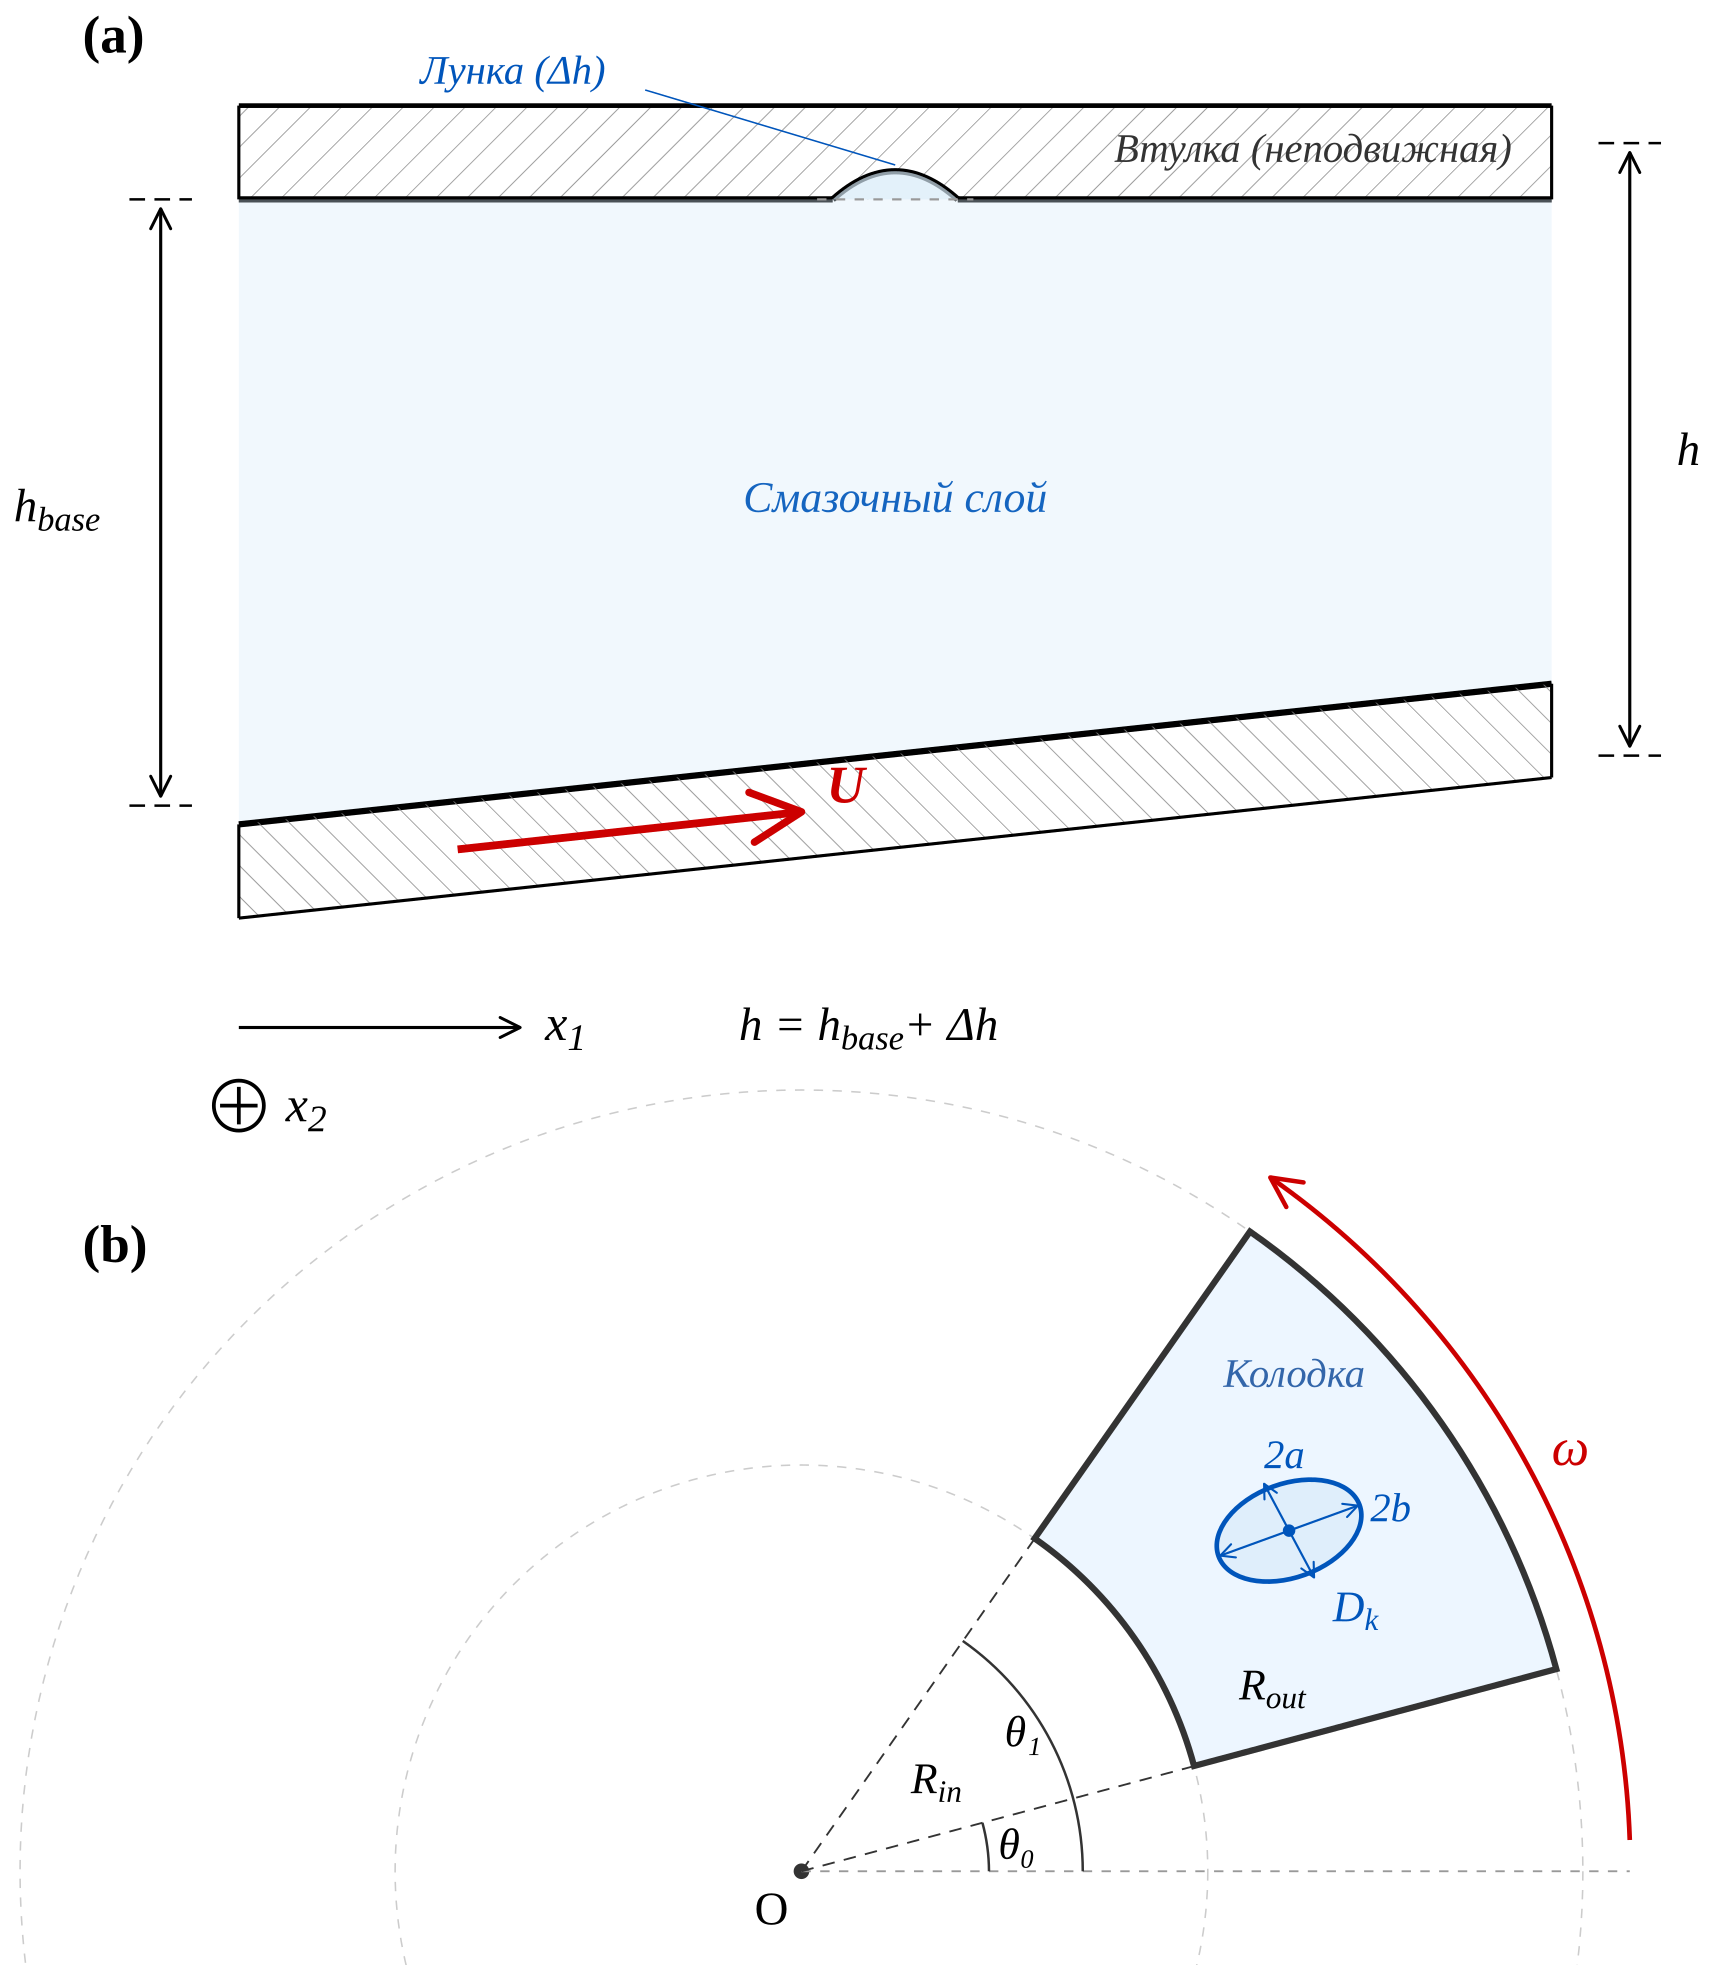
\includegraphics[width=\textwidth,height=0.9\textheight,keepaspectratio]{figures/ch02/fig_2_11.png}
\caption{Суперпозиция толщины зазора: базовый профиль и локальная
  микроструктура}
\label{fig:h_superposition}
\end{figure}

%% ===== Блок 2: Сумма вкладов =====

\subsubsection*{Представление микрорельефа}

Микрорельеф представляется набором из~$N$ локализованных элементов,
вклады которых суммируются:
\begin{equation}
  \Delta h(x_1, x_2)
    = \sum_{k=1}^{N} \Delta h_k(x_1, x_2).
  \label{eq:delta_h_sum}
\end{equation}

Каждый элемент задаётся общим шаблоном (конкретный вид профиля
определяется в подразделе~2.2.2):
\begin{equation}
  \Delta h_k(x_1, x_2)
    = \begin{cases}
        \sigma_k\, h_{p,k}\,
          f_k(x_1 - x_{1,k},\; x_2 - x_{2,k}),
          & (x_1, x_2) \in D_k, \\
        0,
          & (x_1, x_2) \notin D_k,
      \end{cases}
  \label{eq:delta_h_element}
\end{equation}
где:
\begin{itemize}
  \item $D_k$ -- область поддержки (пятно) $k$-го элемента
        на поверхности;
  \item $f_k$ -- профильная функция, задающая форму элемента;
        $f_k(0,0) = 1$;
  \item $\sigma_k = +1$ для углублений (лунок),
        $\sigma_k = -1$ для выступов;
  \item $h_{p,k}$ -- глубина (высота) элемента;
  \item $(x_{1,k},\, x_{2,k})$ -- координаты центра $k$-го элемента.
\end{itemize}

При наличии периодичности по координате $x_1$ (или $x_2$) разность
$x_1 - x_{1,k}$ понимается как минимальная по модулю с учётом
периода~$L_1$ (например, $L_1 = 2\pi R$ для окружного направления).

\paragraph{Эллиптические элементы.}
Для осесимметричных и эллиптических лунок удобно параметризовать
область элемента через безразмерную радиальную координату:
\begin{equation}
  \rho_k
    = \sqrt{
        \left(\frac{x_1 - x_{1,k}}{b_k}\right)^{\!2}
      + \left(\frac{x_2 - x_{2,k}}{a_k}\right)^{\!2}
      }.
  \label{eq:rho_k}
\end{equation}

Тогда $D_k = \{\rho_k \leq 1\}$ -- эллипс с полуосями $b_k$ по~$x_1$
и~$a_k$ по~$x_2$, а профильная функция зависит только от~$\rho$:
$f_k = f(\rho_k)$, причём $f(0) = 1$, $f(1) = 0$.

Для канавок и других неосесимметричных элементов область~$D_k$
и профильная функция~$f_k$ задаются иначе; конкретные формы
рассматриваются в подразделе~2.2.2.

Для однородной текстуры все элементы идентичны
($a_k = a$, $b_k = b$, $h_{p,k} = h_p$, $f_k = f$) и различаются
только положением центров. Типовой элемент с основными обозначениями показан на рис.~\ref{fig:microtexture_params}.

% [РИСУНОК 2.5: Типовая микроструктура с параметрами]
\begin{figure}[!ht]
\centering
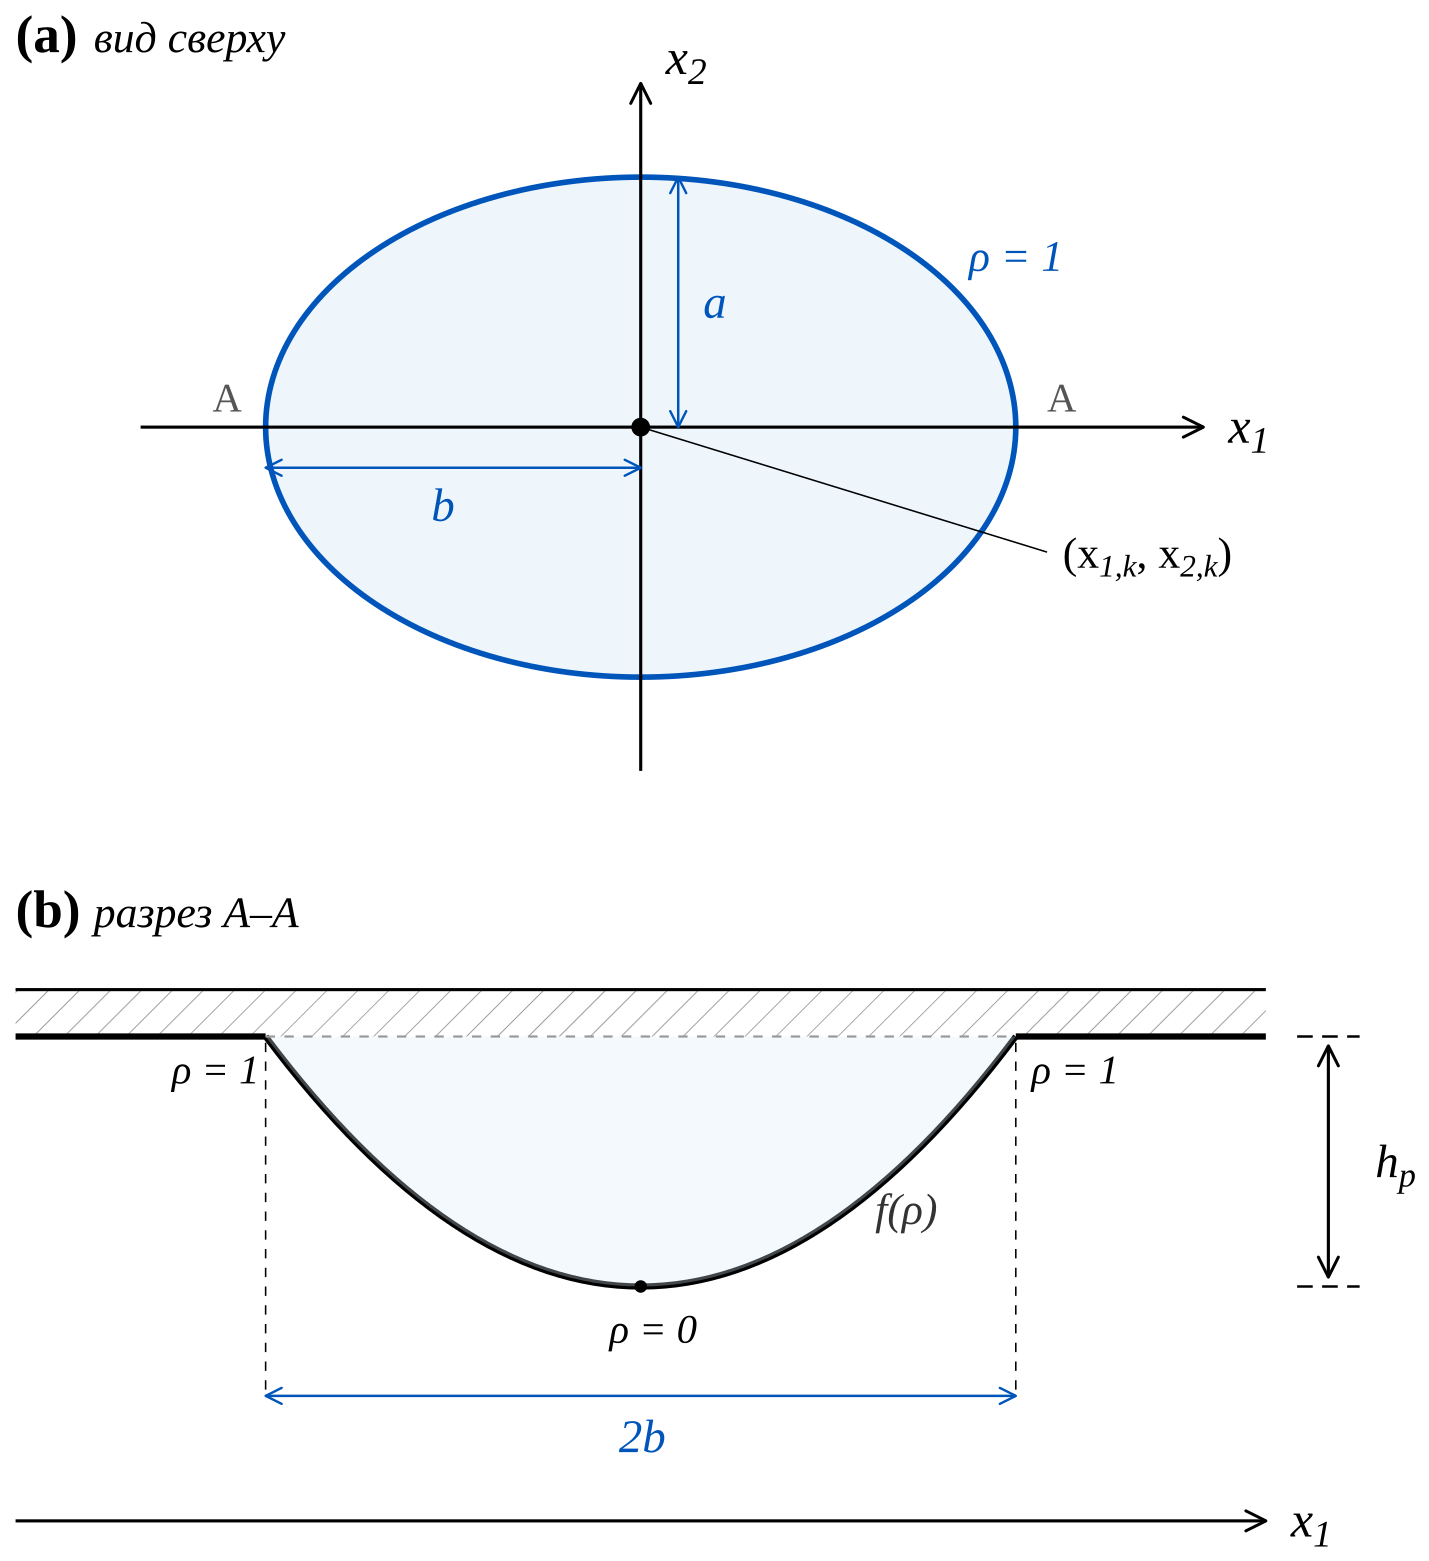
\includegraphics[width=\textwidth,height=0.9\textheight,keepaspectratio]{figures/ch02/fig_2_12.png}
\caption{Типовой элемент микроструктуры с основными геометрическими
  параметрами}
\label{fig:microtexture_params}
\end{figure}

%% ===== Блок 3: Параметры раскладки =====

\subsubsection*{Параметры раскладки}

Положение элементов на поверхности определяется раскладкой. Для её
описания вводятся следующие параметры:
\begin{itemize}
  \item $p_1$, $p_2$ -- шаги раскладки, т.\,е. расстояния между
        центрами соседних элементов по направлениям $x_1$ и~$x_2$;
  \item $N$ -- общее число элементов;
  \item область текстурирования -- участок поверхности, на который
        нанесена текстура (может совпадать со всей расчётной областью
        или быть её частью).
\end{itemize}

Важной интегральной характеристикой является коэффициент заполнения --
доля площади поверхности, занятая элементами:
\begin{equation}
  \phi = \frac{N \cdot A_{\mathrm{elem}}}{A_{\mathrm{tex}}},
  \label{eq:fill_fraction}
\end{equation}
\begin{conditions}
$A_{\mathrm{elem}}$ -- площадь «пятна» одного элемента (для
эллипса $A_{\mathrm{elem}} = \pi a b$);\\
$A_{\mathrm{tex}}$ -- площадь области текстурирования.
\end{conditions}
Конкретные типы решёток (прямоугольная, шахматная, гексагональная
и~др.) и способы задания координат центров рассматриваются
в подразделе~2.2.3.

%% ===== Блок 4: Ограничения модели =====

\subsubsection*{Ограничения модели}

Введённая параметризация корректна при выполнении следующих условий.
\begin{enumerate}
  \item Положительность зазора: $h(x_1, x_2) > 0$ на всей расчётной
        области. Формально:
        $h_{\mathrm{base}}(x_1, x_2) + \Delta h(x_1, x_2) > 0$.
        В частности, при непересекающихся одинаковых лунках достаточно
        $h_p < h_{\mathrm{base,min}}$.
  \item Непересечение элементов:
        $D_k \cap D_{k'} = \varnothing$ для всех $k \neq k'$.
        Для эллиптических элементов без поворота достаточное условие:
        $p_1 \geq 2b$, $p_2 \geq 2a$.
  \item Малая глубина: $h_p / h_0 \ll 1$ обеспечивает применимость
        уравнения Рейнольдса к текстурированной поверхности
        (см.\ подраздел~2.1.5).
  \item Гладкость профиля: непрерывность $\Delta h$ на границе
        элемента ($f(1) = 0$). Желательна также гладкая стыковка
        ($f'(1) = 0$) для уменьшения численных артефактов. Выполнение
        этих условий зависит от выбора профильной функции~$f(\rho)$
        (подраздел~2.2.2).
\end{enumerate}

%% ===== Блок 5: Таблица параметров =====

Полный перечень параметров микроструктуры приведён в табл.~\ref{tab:texture_params}.

\begin{table}[!ht]
\centering
\caption{Параметры детерминированной микроструктуры}
\label{tab:texture_params}
\begin{tabularx}{\textwidth}{|X|c|c|}
\hline
\multicolumn{1}{|c|}{\textbf{Параметр}} & \textbf{Обозначение} & \textbf{Размерность} \\
\hline
Глубина (высота) элемента & $h_p$     & мкм \\
\hline
Полуось по $x_1$ (эллиптич.) & $b$    & мкм \\
\hline
Полуось по $x_2$ (эллиптич.) & $a$    & мкм \\
\hline
Шаг по $x_1$              & $p_1$     & мкм \\
\hline
Шаг по $x_2$              & $p_2$     & мкм \\
\hline
Число элементов           & $N$       & --  \\
\hline
Доля площади (заполнение) & $\phi$    & --  \\
\hline
Профильная функция        & $f(\rho)$ & --  \\
\hline
\end{tabularx}
\end{table}

%% ===== Завершающий абзац =====

Введённая параметрическая модель позволяет описать широкий класс
детерминированных микроструктур~\cite{senatore2018,joshi2018}. Конкретные формы профильной
функции~$f(\rho)$ рассматриваются в подразделе~2.2.2, типы
раскладок -- в подразделе~2.2.3, а переход к безразмерным
параметрам -- в подразделе~2.2.4.

\FloatBarrier
\subsection{Форма микроструктур}

В подразделе~2.2.1 введён общий шаблон элемента микрорельефа:
$\Delta h_k = \sigma_k\, h_{p}\, f_k(\ldots)$ на области~$D_k$.
Цель настоящего подраздела -- задать конкретные профильные
функции~$f$ и формы областей~$D_k$ для всех типов элементов,
используемых в работе. Общие требования к профильной функции
формулируются следующим образом:
\begin{itemize}
  \item $f(0,0) = 1$ (или $f(0) = 1$ для осесимметричных элементов);
  \item $f = 0$ на границе~$D_k$;
  \item желательна непрерывность~$f$ и гладкая стыковка на границе:
        для профилей вида $f(\rho)$ -- $df/d\rho|_{\rho=1} = 0$,
        в общем случае -- $\partial f/\partial n = 0$ на~$\partial D_k$
        (где $n$ -- внешняя нормаль);
  \item $0 \leq f \leq 1$ внутри~$D_k$.
\end{itemize}

%% ===== Блок 1: Локальные координаты =====

\subsubsection*{Локальные координаты элемента}

Для описания элементов произвольной ориентации вводятся локальные
координаты $(\xi, \eta)$, связанные с глобальными $(x_1, x_2)$
поворотом на угол~$\alpha_k$:
\begin{equation}
  \begin{alignedat}{2}
    & \xi  &\;=\;& \phantom{-}(x_1 - x_{1,k})\cos\alpha_k
            + (x_2 - x_{2,k})\sin\alpha_k, \\
    & \eta &\;=\;& -(x_1 - x_{1,k})\sin\alpha_k
            + (x_2 - x_{2,k})\cos\alpha_k.
  \end{alignedat}
  \label{eq:local_coords}
\end{equation}

При $\alpha_k = 0$ локальные координаты совпадают с глобальными. Взаимное расположение осей иллюстрирует рис.~\ref{fig:local_coords}.

Безразмерная радиальная координата для эллиптических элементов
(введённая в подразделе~2.2.1) записывается через локальные
координаты:
\begin{equation}
  \rho_k = \sqrt{\left(\frac{\xi}{b_k}\right)^{\!2}
              +\left(\frac{\eta\vphantom{\xi}}{a_k}\right)^{\!2}}.
  \label{eq:rho_local}
\end{equation}

Область элемента: $D_k = \{\rho_k \leq 1\}$. Для канавок
и прямоугольных элементов область~$D_k$ задаётся иначе (см.\ ниже).

% [РИСУНОК: Локальные координаты элемента]
\begin{figure}[!ht]
\centering
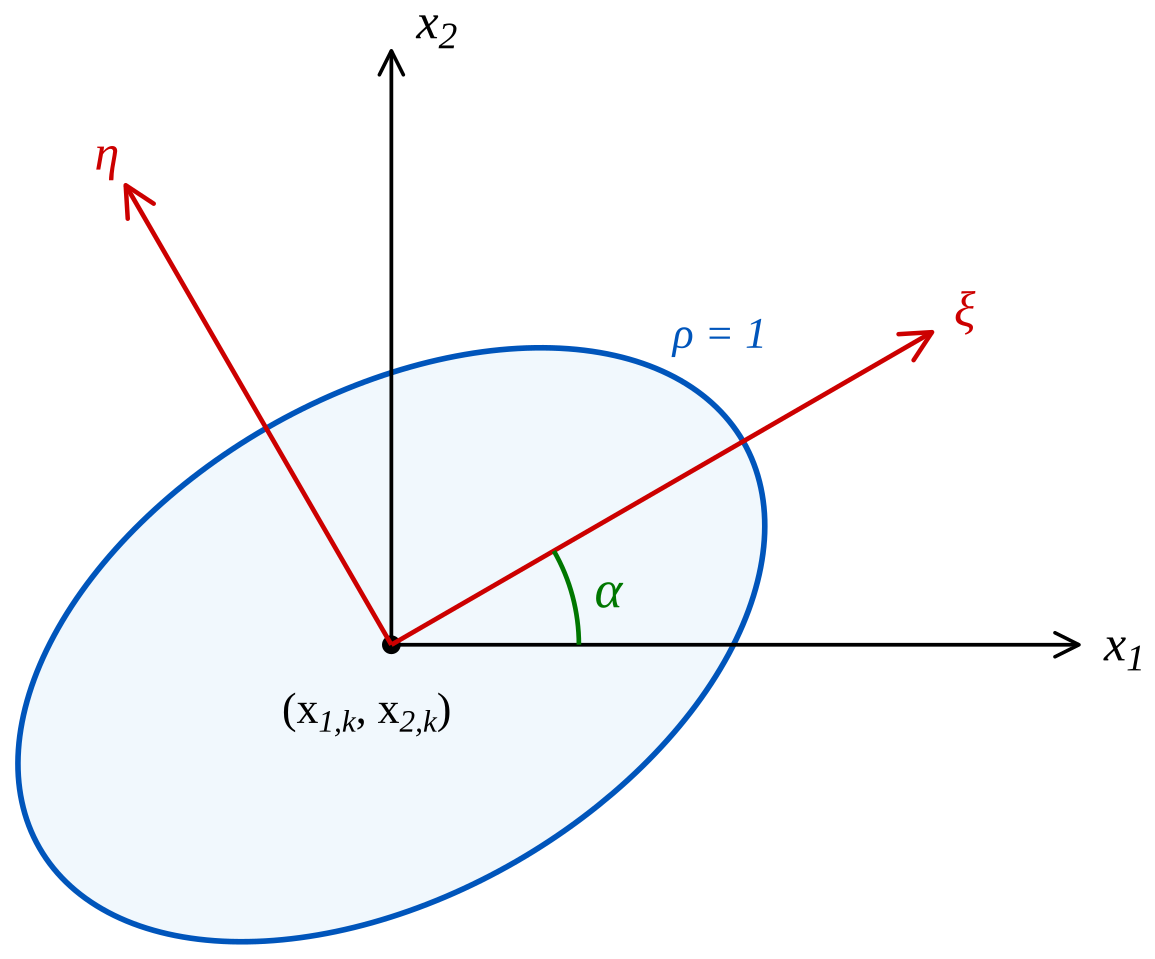
\includegraphics[width=\textwidth,height=0.9\textheight,keepaspectratio]{figures/ch02/fig_2_13.png}
\caption{Локальные координаты элемента микроструктуры и угол поворота}
\label{fig:local_coords}
\end{figure}

%% ===== Блок 2: Осесимметричные и эллиптические профили =====

\subsubsection*{Осесимметричные и эллиптические элементы}

Для элементов с эллиптической областью $D_k = \{\rho_k \leq 1\}$
профильная функция зависит только от~$\rho_k$ (далее для краткости
$\rho$). Ниже приведены основные типы профилей.

\paragraph{A) Эллипсоидальный (полусфероидальная шапка).}
\begin{equation}
  f(\rho) = \sqrt{1 - \rho^2}.
  \label{eq:profile_ellipsoidal}
\end{equation}

Свойства: $f(1) = 0$, но $f'(1) \to -\infty$ (вертикальный обрыв
на границе). При $a = b$ профиль соответствует полусфере. Широко
используется в литературе; на практике разрыв производной обычно
не вызывает проблем при достаточном разрешении сетки.

\paragraph{B) Параболический.}
\begin{equation}
  f(\rho) = 1 - \rho^2.
  \label{eq:profile_parabolic}
\end{equation}

Свойства: $f(1) = 0$, $f'(1) = -2 \neq 0$. Простейший гладкий
профиль. При $a = b$ -- параболоид вращения.

\paragraph{C) Конический (линейный).}
\begin{equation}
  f(\rho) = 1 - \rho.
  \label{eq:profile_conical}
\end{equation}

Свойства: $f(1) = 0$, $df/d\rho|_{\rho=1} = -1$. Как функция
от~$(\xi, \eta)$ через~$\rho$ имеет недифференцируемость в центре
($\rho = 0$), что может приводить к численным артефактам на грубых
сетках.

\paragraph{D) Косинусный.}
\begin{equation}
  f(\rho) = \tfrac{1}{2}\bigl(1 + \cos(\pi\rho)\bigr).
  \label{eq:profile_cosine}
\end{equation}

Свойства: $f(1) = 0$, $f'(1) = 0$. Обеспечивает гладкую стыковку
на границе элемента. Предпочтителен для численных расчётов.

\paragraph{E) Полиномиальный (smoothstep).}
\begin{equation}
  f(\rho) = 1 - 3\rho^2 + 2\rho^3.
  \label{eq:profile_smoothstep}
\end{equation}

Свойства: $f(1) = 0$, $f'(1) = 0$, $f'(0) = 0$. Двусторонняя
гладкость -- и в центре, и на границе.

\paragraph{F) Цилиндрический (плоское дно).}
Вводится параметр $\rho_0$ ($0 < \rho_0 < 1$) -- радиус плоского
участка:
\begin{equation}
  f(\rho) =
    \begin{cases}
      1,
        & 0 \leq \rho \leq \rho_0, \\[4pt]
      g\!\left(\dfrac{\rho - \rho_0}{1 - \rho_0}\right),
        & \rho_0 < \rho \leq 1,
    \end{cases}
  \label{eq:profile_plateau}
\end{equation}
где $g(t)$ -- функция перехода от~1 к~0 на отрезке $t \in [0,\,1]$.
Общие требования: $g(0) = 1$, $g(1) = 0$; для гладкой стыковки
на внешней границе дополнительно $g'(1) = 0$ (и желательно
$g'(0) = 0$, что обеспечивает плавный переход от плоского участка
к наклонной стенке).
Примеры: $g(t) = 1 - t^2$ (параболический переход, без гладкой
стыковки по наклону),
$g(t) = \frac{1}{2}(1 + \cos\pi t)$ (гладкий косинусный переход).

При $\rho_0 \to 0$ профиль вырождается в соответствующий «обычный»
тип; при $\rho_0 \to 1$ -- приближается к цилиндрическому с резкими
стенками. Параметр~$\rho_0$ позволяет моделировать лунки с плоским
дном, характерные для лазерного текстурирования. При $a = b$ и без
функции перехода ($g$ -- ступенька) элемент представляет собой
круговой цилиндр; при $a \neq b$ -- эллиптический цилиндр.

%% ===== Блок 3: Канавки =====

\subsubsection*{Канавки}

Для канавок область~$D_k$ -- прямоугольник в локальных координатах:
\begin{equation}
  D_k = \bigl\{|\xi| \leq \ell/2,\; |\eta| \leq a\bigr\},
  \label{eq:groove_Dk}
\end{equation}
\begin{conditions}
$\ell$ -- длина канавки (вдоль~$\xi$);\\
$a$ -- полуширина (по~$\eta$).
\end{conditions}
Профильная функция задаётся по поперечному направлению~$\eta$
(вдоль~$\xi$ профиль постоянен):
\begin{equation}
  f_k(\xi, \eta) = f_\perp\!\bigl(|\eta|/a\bigr),
  \label{eq:groove_profile}
\end{equation}
где $f_\perp(t)$, $t \in [0,\,1]$ -- поперечный профиль.

При необходимости гладкого замыкания канавки по концам вводится
продольное окно:
\begin{equation}
  f_k(\xi, \eta)
    = f_\parallel\!\bigl(|\xi|/(\ell/2)\bigr)
      \cdot f_\perp\!\bigl(|\eta|/a\bigr),
  \label{eq:groove_profile_window}
\end{equation}
где $f_\parallel(s)$, $s \in [0,\,1]$ -- продольный профиль
с условиями $f_\parallel(0) = 1$, $f_\parallel(1) = 0$. Например,
$f_\parallel(s) = \frac{1}{2}(1 + \cos\pi s)$. Для канавок
с резкими торцами полагают $f_\parallel \equiv 1$.

Примеры поперечного профиля:
параболический $f_\perp(t) = 1 - t^2$,
косинусный $f_\perp(t) = \frac{1}{2}(1 + \cos\pi t)$,
прямоугольный $f_\perp(t) = 1$.
Прямоугольный профиль $f_\perp(t) = 1$ соответствует ступенчатому
разрыву на границе элемента и используется для моделирования канавок
с резкими стенками; при необходимости гладкой стыковки следует
выбирать $f_\perp(1) = 0$.

Ориентация канавки задаётся углом~$\alpha_k$ через формулы локальных
координат~\eqref{eq:local_coords}. При $\alpha_k = 0$ канавка
ориентирована вдоль~$x_1$ (продольная), при $\alpha_k = \pi/2$ --
вдоль~$x_2$ (поперечная). Дополнительным параметром канавки является
её длина~$\ell$.

%% ===== Блок 4: Сводная таблица =====

\subsubsection*{Сводка типов профилей}

Основные типы профильных функций и их свойства приведены
в таблице~\ref{tab:profile_types}; сравнение форм профилей показано на рис.~\ref{fig:profile_comparison}, а общий вид элементов -- на рис.~\ref{fig:texture_geometries}.

\begin{table}[!ht]
\centering
\caption{Типы профильных функций элементов микрорельефа}
\label{tab:profile_types}
\small
\begin{tabular}{|p{3.0cm}|c|c|c|p{3.8cm}|}
\hline
\textbf{Тип} & \textbf{Профильная функция}
  & $\boldsymbol{f(1){=}0}$ & $\boldsymbol{df/d\rho|_{1}{=}0}$
  & \textbf{Комментарий} \\
\hline
Эллипсоидальный & $\sqrt{1-\rho^2}$
  & да & нет & $f' \to -\infty$ на границе \\
\hline
Параболический & $1-\rho^2$
  & да & нет & простейший гладкий \\
\hline
Конический & $1-\rho$
  & да & нет & излом в центре \\
\hline
Косинусный & $\frac{1}{2}(1+\cos\pi\rho)$
  & да & да & гладкая стыковка \\
\hline
Smoothstep & $1-3\rho^2+2\rho^3$
  & да & да & гладкость с~обеих сторон \\
\hline
Плоское дно & кусочная (см.\ текст)
  & да & зависит от~$g$ & лазерные лунки \\
\hline
Канавка & $f_\perp(|\eta|/a)$
  & -- & -- & профиль по~$\eta$ \\
\hline
\end{tabular}
\end{table}

%% ===== Блок 5: Рисунки =====

% [РИСУНОК: Сравнение профилей f(ρ)]
\begin{figure}[!ht]
\centering
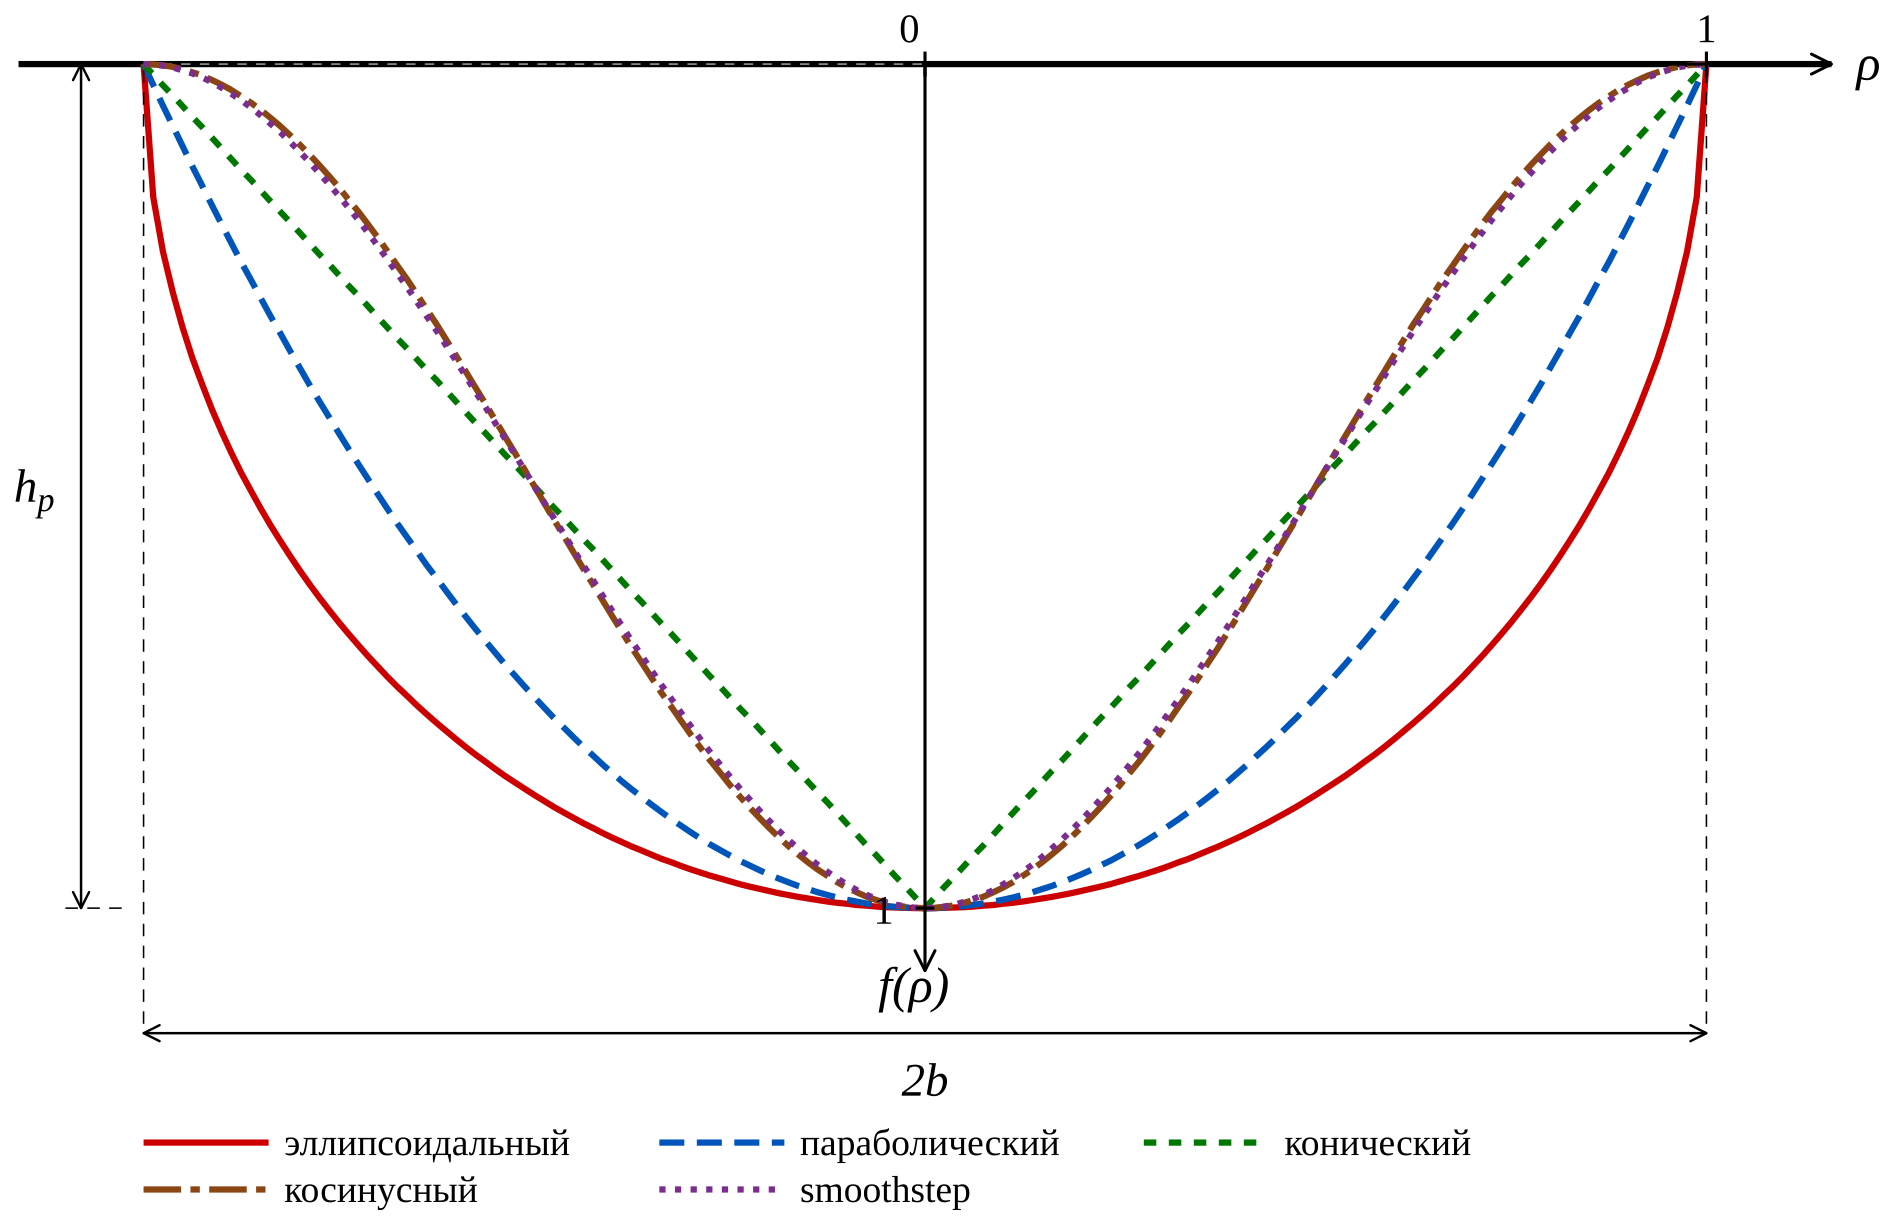
\includegraphics[width=\textwidth,height=0.9\textheight,keepaspectratio]{figures/ch02/fig_2_14.png}
\caption{Сравнение профильных функций элементов микрорельефа}
\label{fig:profile_comparison}
\end{figure}

% [РИСУНОК: Типы микроструктур (обновлённый)]
\begin{figure}[!ht]
\centering
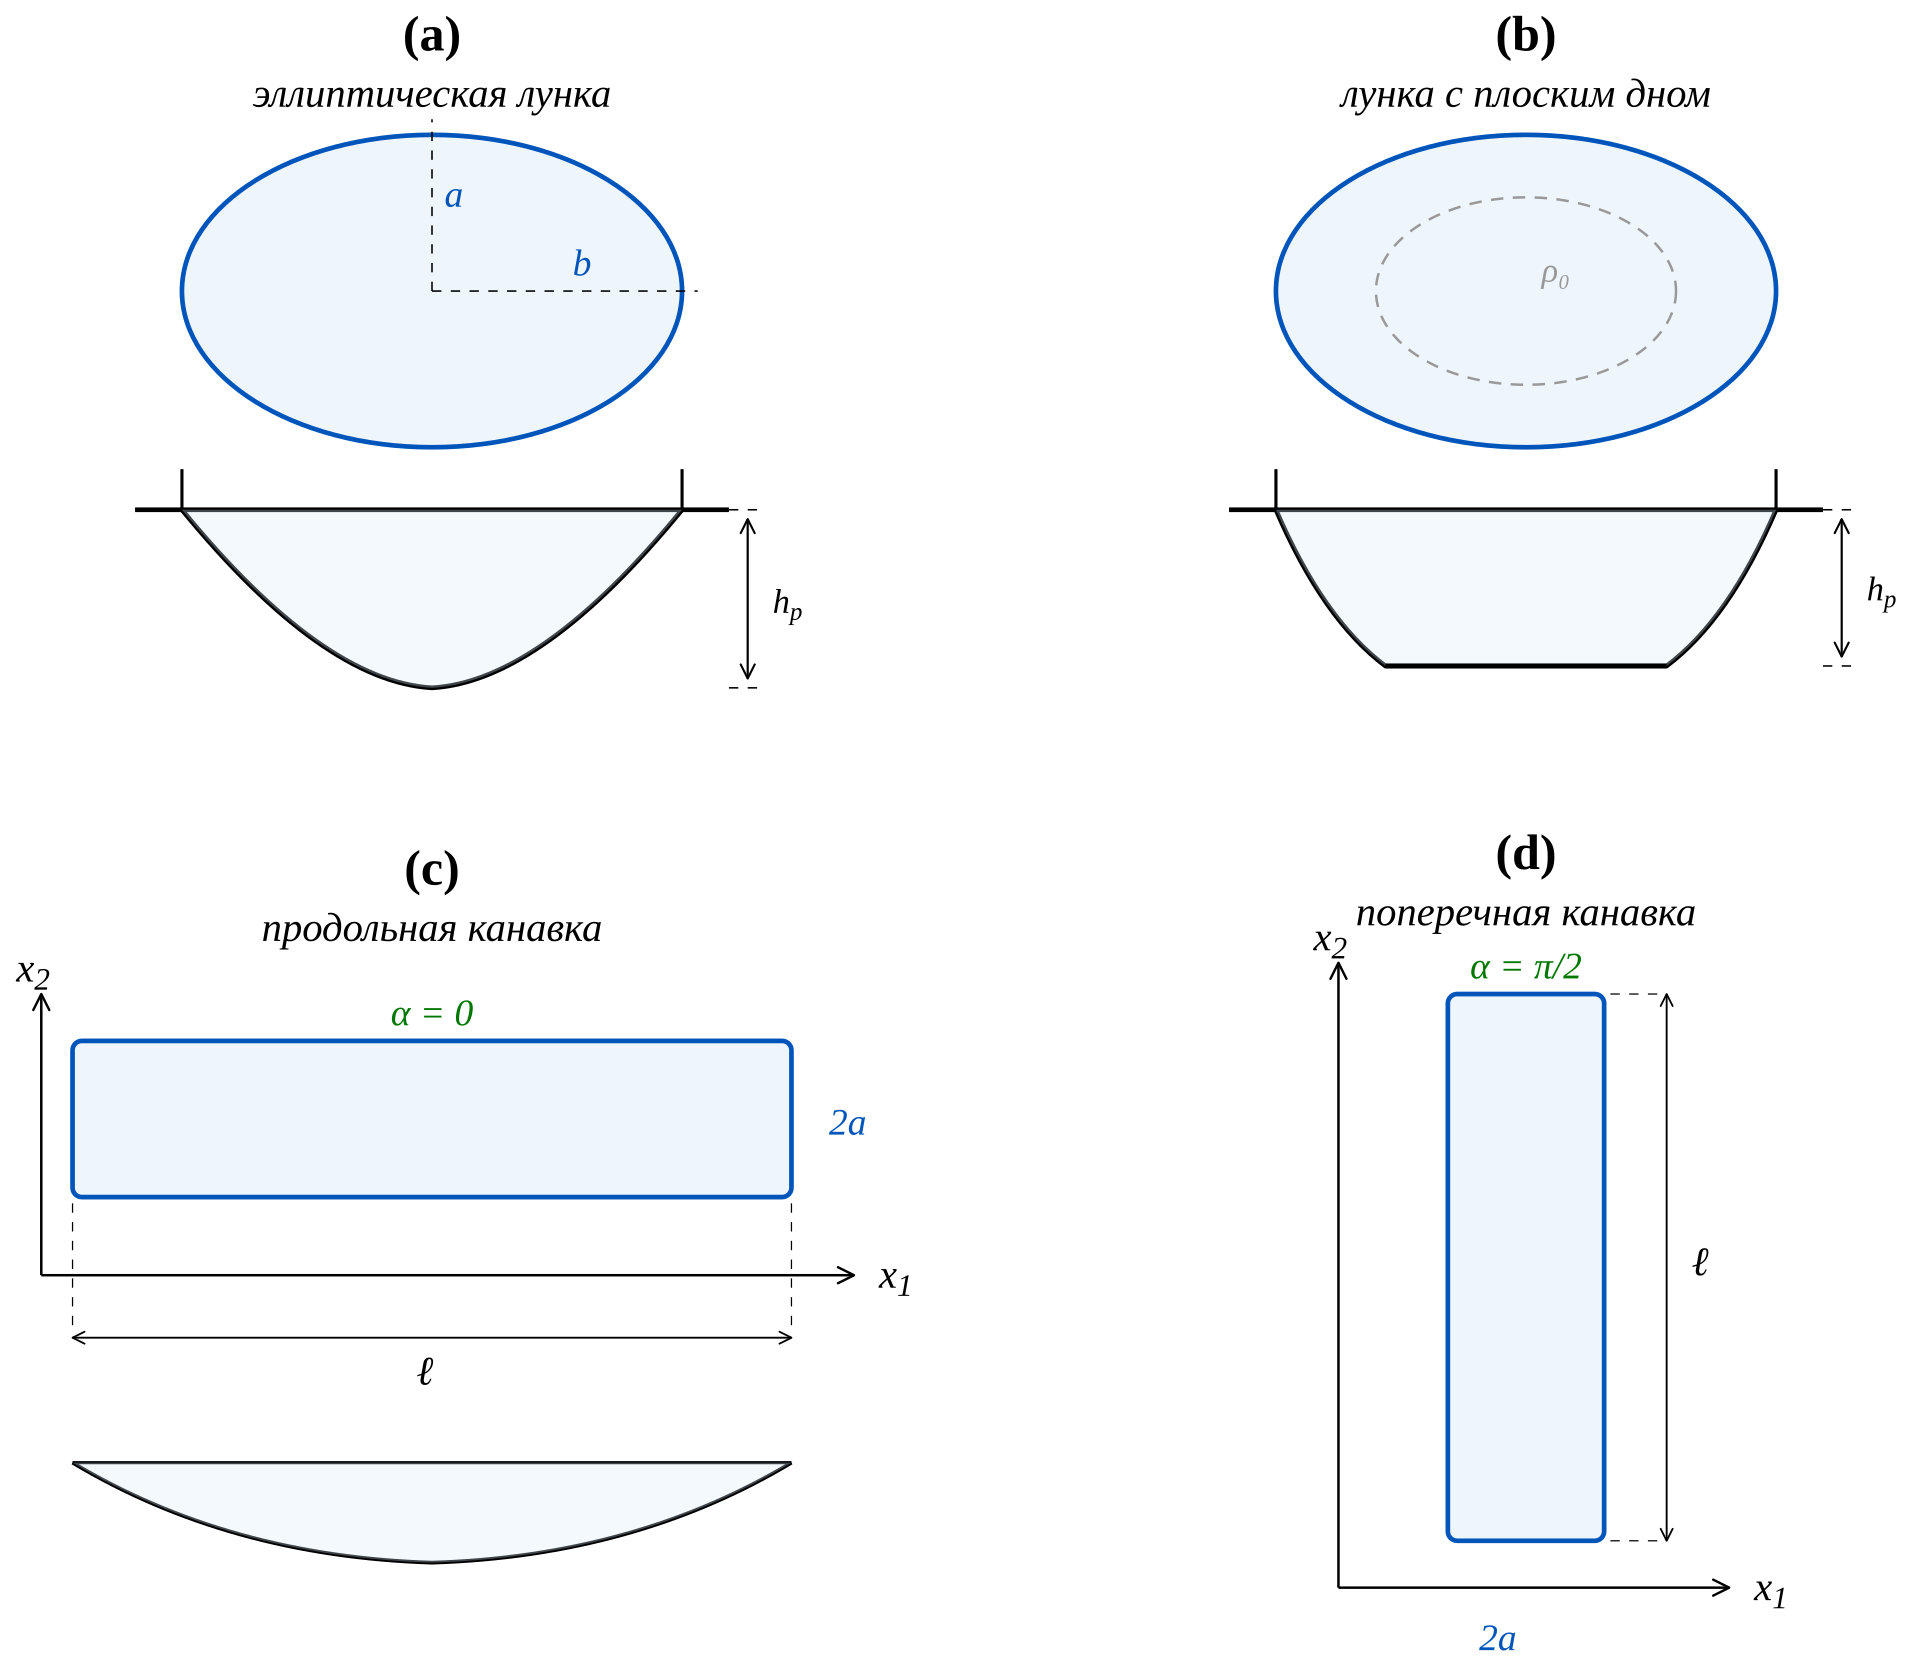
\includegraphics[width=\textwidth,height=0.9\textheight,keepaspectratio]{figures/ch02/fig_2_15.png}
\caption{Основные типы элементов микрорельефа}
\label{fig:texture_geometries}
\end{figure}

%% ===== Завершающий абзац =====

Приведённый набор профильных функций охватывает основные типы
элементов, используемых в практике текстурирования подшипников
скольжения. Выбор конкретного профиля определяется технологией
изготовления и требованиями к гладкости численного решения~\cite{senatore2018,qiangli2019,yujun2023,gropper2018}.
Пространственное расположение элементов на поверхности
рассматривается в подразделе~2.2.3.

\FloatBarrier
\subsection{Варианты расположения микроструктур}

Геометрия отдельного элемента микрорельефа задана
в подразделе~2.2.2. Настоящий подраздел определяет способы
расположения элементов на рабочей поверхности. Результат --
множество центров $\{(x_{1,k},\, x_{2,k})\}_{k=1}^{N}$ (и при
необходимости углов поворота~$\alpha_k$ для канавок). Раскладка
задаётся на прямоугольной области текстурирования
$\Omega_{\mathrm{tex}}
  = [x_{1,s},\, x_{1,t}] \times [x_{2,s},\, x_{2,t}]$
в поверхностных координатах~$(x_1, x_2)$. По периодическому
направлению (например, $x_1 = R\theta$ с периодом $L_1 = 2\pi R$)
координаты центров вычисляются с учётом периодичности по~$x_1$.

%% ===== Блок 1: Прямоугольная решётка =====

\subsubsection*{Прямоугольная решётка}

Базовый тип раскладки. Центры расположены в узлах прямоугольной
сетки с шагами~$p_1$, $p_2$ и начальными смещениями~$\delta_1$,
$\delta_2$:
\begin{equation}
  x_{1,i} = x_{1,s} + \delta_1 + i\,p_1, \quad
  x_{2,j} = x_{2,s} + \delta_2 + j\,p_2,
  \label{eq:layout_rect}
\end{equation}
где $i = 0, 1, \ldots, I_{\max}$; $j = 0, 1, \ldots, J_{\max}$.
Обычно выбирают $0 \leq \delta_1 < p_1$,
$0 \leq \delta_2 < p_2$. Тогда
\[
  I_{\max}
    = \left\lfloor \frac{x_{1,t} - x_{1,s} - \delta_1}{p_1} \right\rfloor,
  \quad
  J_{\max}
    = \left\lfloor \frac{x_{2,t} - x_{2,s} - \delta_2}{p_2} \right\rfloor.
\]

Площадь элементарной ячейки:
$S_{\mathrm{cell}} = p_1 \cdot p_2$.
Коэффициент заполнения (связь с формулой~\eqref{eq:fill_fraction}
из подраздела~2.2.1):
\begin{equation}
  \phi \approx \frac{A_{\mathrm{elem}}}{p_1\,p_2}.
  \label{eq:fill_rect}
\end{equation}

%% ===== Блок 2: Шахматная решётка =====

\subsubsection*{Шахматная решётка}

Чётные и нечётные ряды сдвинуты друг относительно друга на
половину шага по~$x_1$:
\begin{equation}
  \begin{alignedat}{2}
    & x_{2,j}   &\;=\;& x_{2,s} + \delta_2 + j\,p_2, \\
    & x_{1,i,j} &\;=\;& x_{1,s} + \delta_1 + i\,p_1
                  + \tfrac{1}{2}\,p_1\,(j \bmod 2).
  \end{alignedat}
  \label{eq:layout_staggered}
\end{equation}

Индекс~$i$ для фиксированного~$j$ выбирается так, чтобы
$x_{1,i,j} \in [x_{1,s},\, x_{1,t}]$.
Шахматная раскладка повышает равномерность покрытия при тех же
шагах~$p_1$, $p_2$. Площадь элементарной ячейки та же:
$S_{\mathrm{cell}} = p_1 \cdot p_2$.

%% ===== Блок 3: Гексагональная решётка =====

\subsubsection*{Гексагональная решётка}

Является частным случаем шахматной раскладки с определённым
соотношением шагов. Задаётся одним параметром -- расстоянием между
ближайшими центрами~$p$:
\begin{equation}
  p_1 = p, \quad p_2 = \frac{\sqrt{3}}{2}\,p.
  \label{eq:layout_hex}
\end{equation}

Формулы координат -- как для шахматной
решётки~\eqref{eq:layout_staggered} с этими шагами.
Гексагональная раскладка обеспечивает наиболее плотную упаковку
круговых элементов ($a = b$) на плоскости. Площадь элементарной ячейки:
$S_{\mathrm{cell}} = p_1\,p_2 = \frac{\sqrt{3}}{2}\,p^2$.
Соответствующая оценка коэффициента заполнения:
\[
  \phi \approx \frac{A_{\mathrm{elem}}}{S_{\mathrm{cell}}}
    = \frac{2\,A_{\mathrm{elem}}}{\sqrt{3}\,p^2}.
\]

%% ===== Блок 4: Филлотаксис =====

\subsubsection*{Спиральная раскладка (филлотаксис)}

Центры элементов располагаются по спирали Ферма с шагом по углу,
равным золотому углу $\gamma = 2\pi(2 - \varphi)$, где
$\varphi = (1 + \sqrt{5})/2$ -- золотое сечение:
\begin{equation}
  \begin{aligned}
    r_k      &= c\,\sqrt{k}, \\
    \theta_k &= k\,\gamma,
  \end{aligned}
  \quad k = 1, 2, \ldots, N,
  \label{eq:layout_phyllotaxis}
\end{equation}
где $c$ -- масштабный коэффициент, определяющий расстояние между
витками (связан с требуемой плотностью заполнения). Площадь,
приходящаяся на один элемент, приближённо равна $\pi c^2$, откуда
\begin{equation}
  c \approx \sqrt{\frac{A_{\mathrm{tex}}}{\pi\,N}}.
  \label{eq:phyllotaxis_c}
\end{equation}

Координаты
центров в поверхностных координатах $(x_{1,k},\, x_{2,k})$
пересчитываются из $(r_k, \theta_k)$ в зависимости от постановки.

Филлотаксис обеспечивает равномерное заполнение круговой или
кольцевой области без выраженных рядов и столбцов. Раскладка
особенно удобна для кольцевых областей (упорный подшипник).

%% ===== Блок 5: Раскладка канавок =====

\subsubsection*{Раскладка канавок}

Для канавок раскладка упрощается: центры располагаются вдоль одного
направления с постоянным шагом. Например, для канавок,
ориентированных вдоль~$x_1$ ($\alpha_k = 0$), центры задаются как
\[
  x_{2,k} = x_{2,s} + \delta_2 + k\,p_2,
  \quad k = 0, 1, \ldots, N_g - 1,
\]
а $x_{1,k} = (x_{1,s} + x_{1,t})/2$. Для сквозных канавок по всему
периодическому направлению длина $\ell = L_1$.
Для перекрёстных канавок (например, продольные + поперечные)
задаются два семейства с разными углами~$\alpha$.

Основные типы регулярных раскладок показаны на рис.~\ref{fig:layout_staggered}; спиральная раскладка по принципу филлотаксиса -- на рис.~\ref{fig:layout_phyllotaxis}.

%% ===== Блок 6: Рисунки =====

% [РИСУНОК: Типы решёток]
\begin{figure}[!ht]
\centering
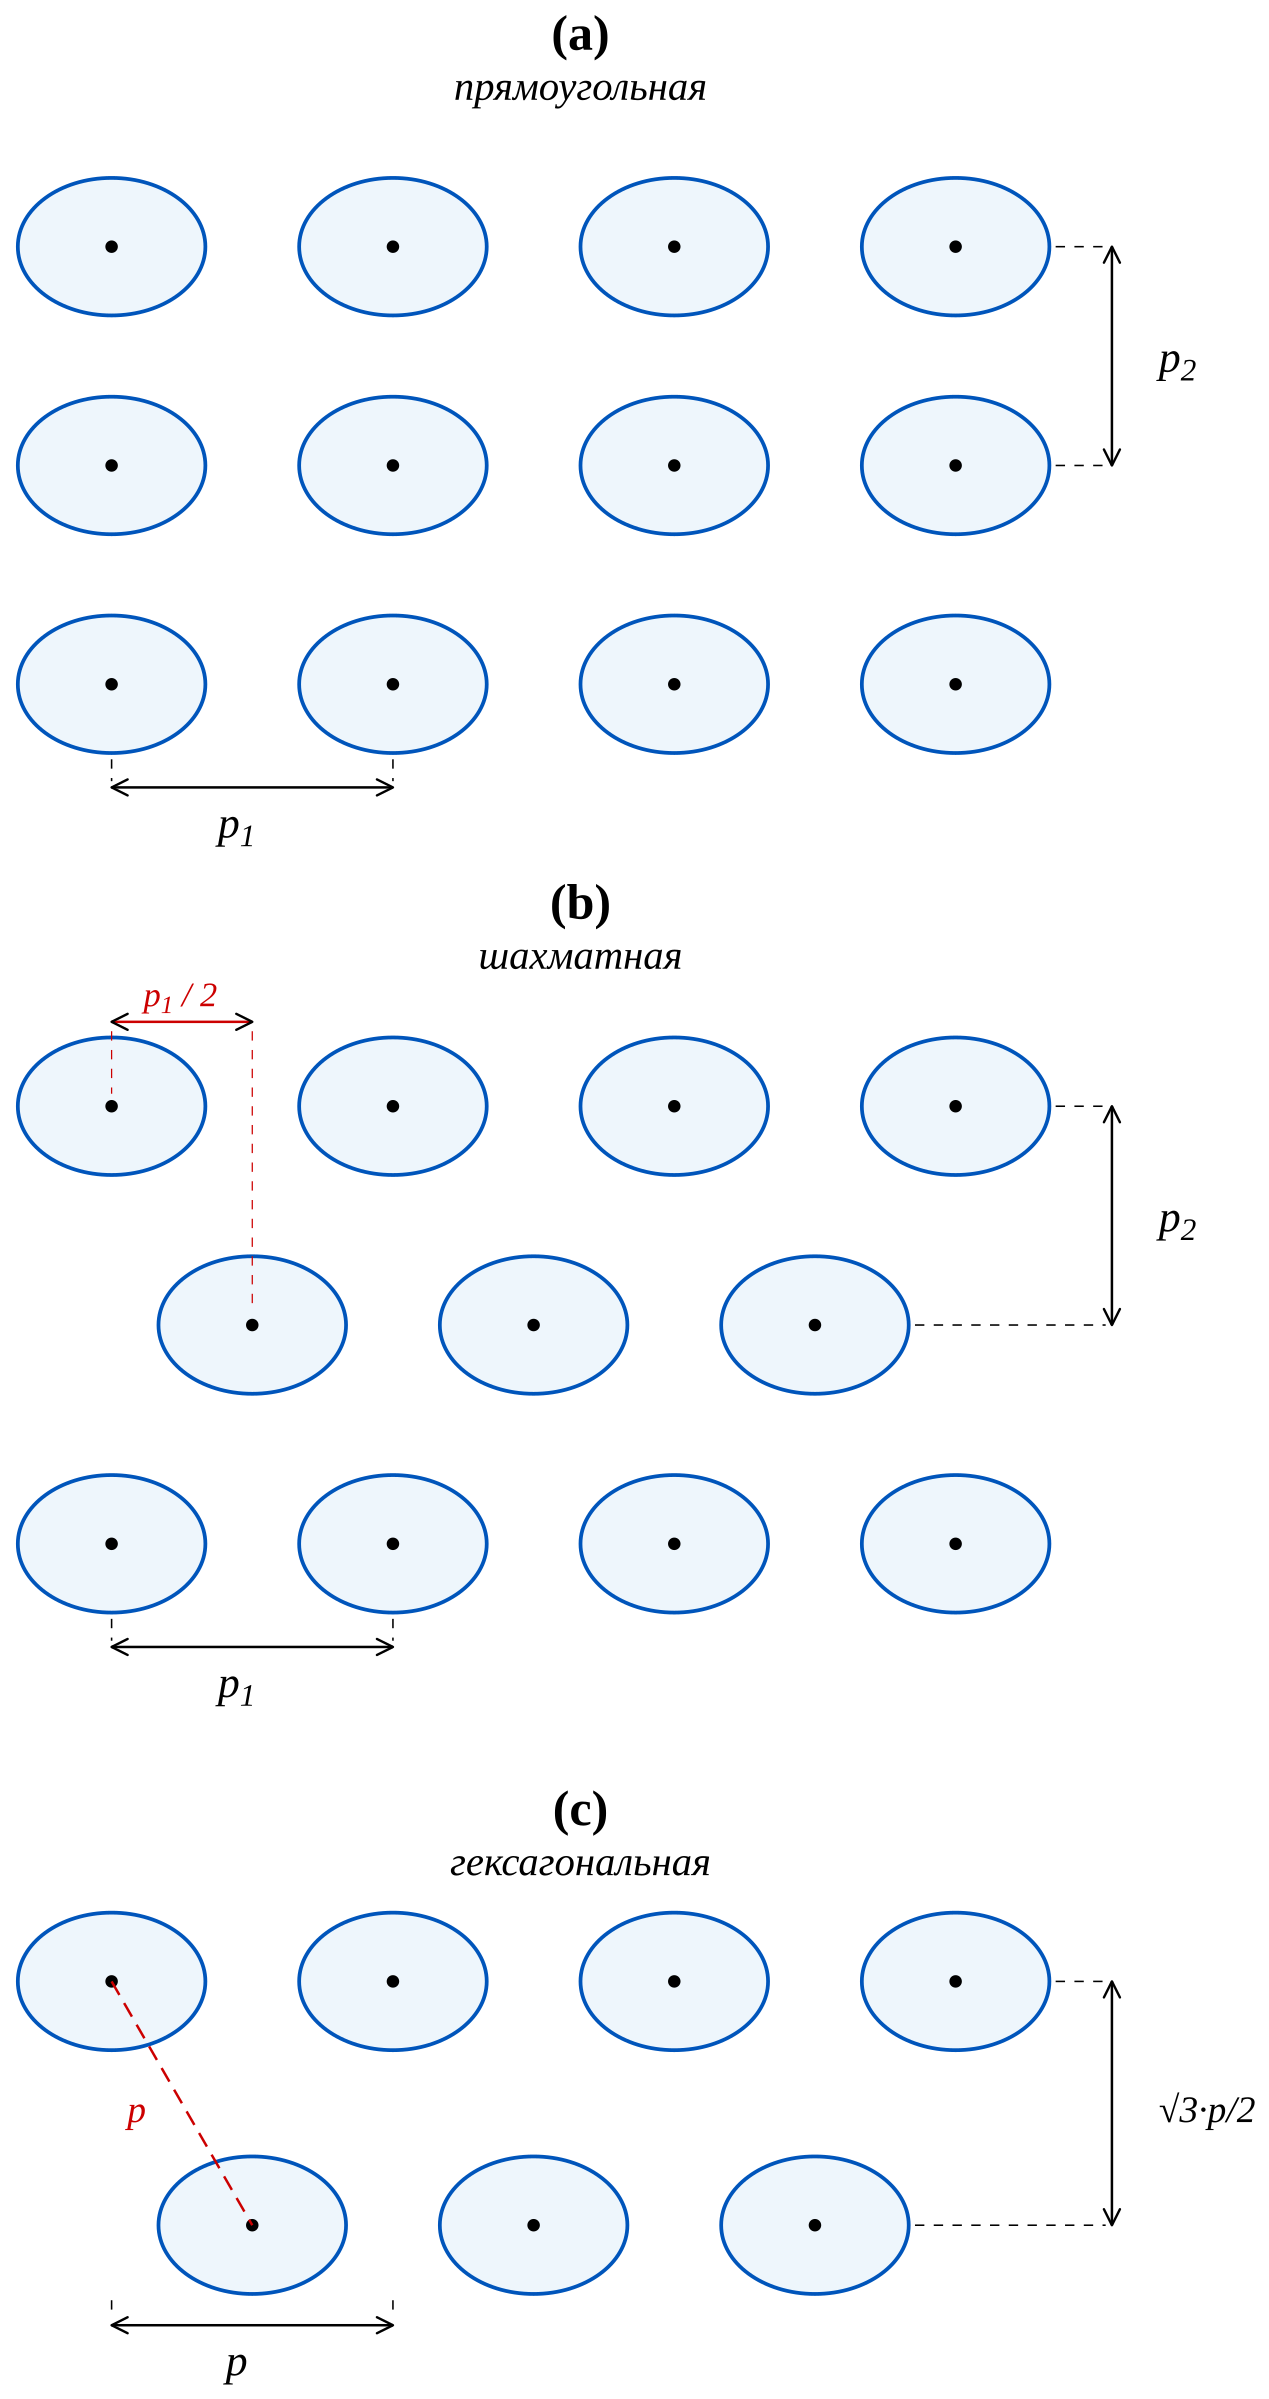
\includegraphics[width=\textwidth,height=0.9\textheight,keepaspectratio]{figures/ch02/fig_2_16.png}
\caption{Основные типы регулярных раскладок микроструктур}
\label{fig:layout_staggered}
\end{figure}

% [РИСУНОК: Филлотаксис]
\begin{figure}[!ht]
\centering
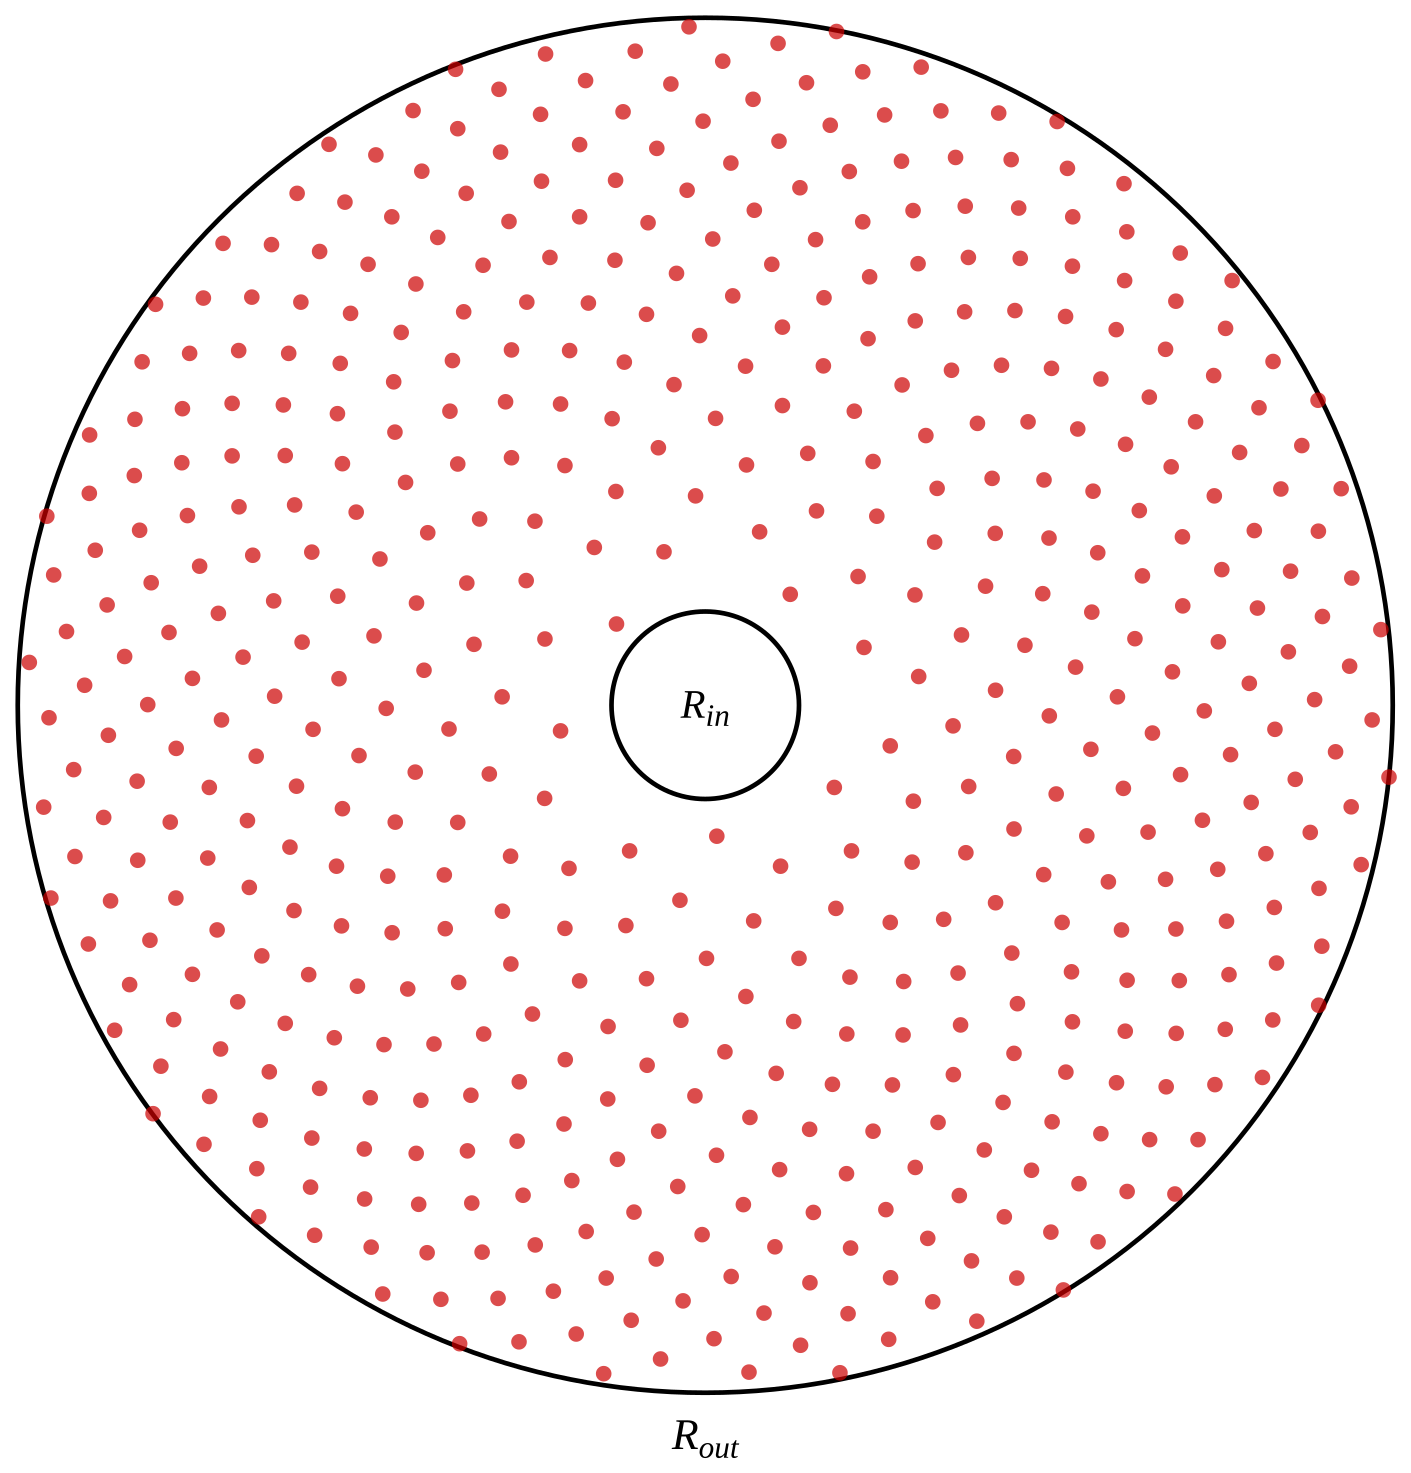
\includegraphics[width=\textwidth,height=0.9\textheight,keepaspectratio]{figures/ch02/fig_2_17.png}
\caption{Раскладка микроструктур по принципу филлотаксиса}
\label{fig:layout_phyllotaxis}
\end{figure}

%% ===== Правило включения центров =====

В настоящей работе элемент считается принадлежащим области
текстурирования, если его центр $(x_{1,k},\, x_{2,k})$ лежит
в~$\Omega_{\mathrm{tex}}$. При необходимости исключения элементов,
частично выходящих за границу, дополнительно требуют, чтобы
область~$D_k$ целиком помещалась в~$\Omega_{\mathrm{tex}}$, что
эквивалентно введению защитных отступов порядка~$a_k$, $b_k$ от границ
области (для однородной текстуры -- $a$, $b$).

%% ===== Завершающий абзац =====

Выбор типа раскладки определяется формой области текстурирования,
типом подшипника и целями параметрического анализа~\cite{senatore2018}. Безразмерные
параметры, характеризующие микрорельеф в целом, вводятся
в подразделе~2.2.4.

\FloatBarrier
\subsection{Безразмерные параметры микрорельефа}

Для параметрического анализа удобно перейти к безразмерным параметрам текстуры.
Используются масштабы, введённые в подразделе~2.1.6
(таблица~\ref{tab:nondim_scales}): характерная толщина зазора~$h_0$
и характерные длины~$L_1$,~$L_2$ по поверхностным координатам~$x_1$,~$x_2$.
Безразмерные координаты и уравнение Рейнольдса уже заданы
в подразделе~2.1.6; здесь нормируются только параметры текстуры.

Ключевым безразмерным параметром является отношение глубины элемента
к характерной толщине зазора:
\begin{equation}\label{eq:Hp_nondim}
  H_p = \frac{h_p}{h_0}.
\end{equation}

Требование применимости уравнения Рейнольдса к текстурированной
поверхности (подраздел~2.1.5) формулируется как $H_p \ll 1$.

Безразмерные полуоси элемента определяются делением на соответствующие
масштабы длины:
\begin{equation}\label{eq:AB_nondim}
  A^{*} = \frac{a}{L_2}, \quad B^{*} = \frac{b}{L_1},
\end{equation}
аспектное отношение элемента:
\begin{equation}\label{eq:kappa}
  \kappa = \frac{a}{b}.
\end{equation}

При $\kappa = 1$ элемент осесимметричен (круговая лунка);
при $\kappa \neq 1$ -- эллиптический.
Заметим, что при $L_1 \neq L_2$ выполняется
\[
  \kappa = \frac{a}{b}
         = \frac{A^{*}}{B^{*}}\,\frac{L_2}{L_1},
\]
а при $L_1 = L_2$ получаем $\kappa = A^{*}/B^{*}$.

Безразмерные шаги раскладки:
\begin{equation}\label{eq:P_nondim}
  P_1^{*} = \frac{p_1}{L_1}, \quad P_2^{*} = \frac{p_2}{L_2}.
\end{equation}

Условия непересечения элементов (подраздел~2.2.1) удобно проверять
через отношения $p_1/(2b)$ и $p_2/(2a)$, которые показывают,
во сколько раз шаг превышает полный размер элемента
($2b$ по $x_1$ и $2a$ по $x_2$).

Коэффициент заполнения~$\phi$ (подраздел~2.2.1) является безразмерным.
Для эллиптических элементов на регулярной решётке при непересекающихся
элементах и пренебрежении краевыми эффектами
\begin{equation}\label{eq:phi_nondim}
  \phi \approx \frac{\pi\, a\, b}{p_1\, p_2}
       = \frac{\pi\, A^{*}\, B^{*}}{P_1^{*}\, P_2^{*}}.
\end{equation}

Полный перечень безразмерных параметров микрорельефа сведён в табл.~\ref{tab:nondim_texture}.

Ряд параметров текстуры является безразмерным по определению:
$\rho_0 \in (0,\,1)$ -- параметр плоского дна (подраздел~2.2.2);
$\alpha$ -- угол ориентации элемента.
Для канавок вводится безразмерная длина $\ell^{*} = \ell / L_1$;
для сквозных канавок по периодическому направлению при выборе
$L_1$ равным длине периода $\ell^{*} = 1$.
Для повёрнутых элементов ($\alpha \neq 0$) используются локальные
координаты из подраздела~2.2.2; переход к безразмерным величинам
выполняется делением длин на соответствующие масштабы из~2.1.6.

\begin{table}[!ht]
\centering
\caption{Безразмерные параметры микрорельефа}
\label{tab:nondim_texture}
\begin{tabularx}{\textwidth}{|X|c|c|}
\hline
\multicolumn{1}{|c|}{\textbf{Параметр}} & \textbf{Обозначение} & \textbf{Определение} \\
\hline
Безразмерная глубина             & $H_p$    & $h_p / h_0$                          \\
\hline
Безразмерная полуось по $x_2$    & $A^{*}$  & $a / L_2$                            \\
\hline
Безразмерная полуось по $x_1$    & $B^{*}$  & $b / L_1$                            \\
\hline
Отношение полуосей               & $\kappa$ & $a / b$                              \\
\hline
Безразмерный шаг по $x_1$        & $P_1^{*}$ & $p_1 / L_1$                        \\
\hline
Безразмерный шаг по $x_2$        & $P_2^{*}$ & $p_2 / L_2$                        \\
\hline
Коэффициент заполнения           & $\phi$   & $N A_{\mathrm{elem}} / A_{\mathrm{tex}}$ \\
\hline
Параметр плоского дна            & $\rho_0$ & $(0,\,1)$                            \\
\hline
Угол ориентации                  & $\alpha$ & --                                   \\
\hline
Безразмерная длина канавки       & $\ell^{*}$ & $\ell / L_1$                       \\
\hline
\end{tabularx}
\end{table}

\FloatBarrier

Введённый набор безразмерных параметров
($H_p$, $A^{*}$, $B^{*}$, $\kappa$, $P_1^{*}$, $P_2^{*}$, $\phi$, $\rho_0$, $\ell^{*}$)
позволяет проводить параметрические исследования и сравнивать результаты
для различных типов подшипников при одинаковых безразмерных группах.

Физический смысл каждого безразмерного параметра элемента
микрорельефа целесообразно кратко прокомментировать.
Глубина~$H_p = h_p/h_0$ задаёт масштаб добавки к зазору
относительно характерной толщины плёнки. При $H_p \ll 1$
лунка неглубокая; её гидродинамический эффект мал, так как
создаваемый ею дополнительный клин пропорционален $H_p$.
При $H_p \gtrsim 1$ глубина лунки сопоставима с зазором,
что может нарушить течение в соседних ячейках и снизить
несущую способность; для эллипсоидальных лунок оптимальная
глубина, как правило, находится в диапазоне
$H_p \approx 0{,}2$--$0{,}5$.

Безразмерные полуоси~$A^{*}$, $B^{*}$ задают размеры элемента
относительно длин расчётной области в каждом из координатных
направлений. Произведение~$\pi A^{*} B^{*}$ пропорционально
безразмерной площади одной лунки; коэффициент
покрытия~$\phi$ определяет суммарную долю текстурированной
площади. Ориентация эллипса ($A^{*} \neq B^{*}$) влияет
на анизотропию гидродинамического эффекта и, следовательно,
на соотношение между несущей способностью, трением и утечками.

Шаги~$P_1^{*}$, $P_2^{*}$ (периоды раскладки по~$s_1$
и~$s_2$ соответственно) совместно с~$A^{*}$, $B^{*}$
и~$\phi$ образуют замкнутый набор параметров текстуры,
достаточный для однозначного задания шахматной раскладки.
При шахматной схеме реальный шаг в нечётных рядах сдвигается
на $P_1^{*}/2$, что обеспечивает более равномерное перекрытие
поверхности при той же плотности.

\textit{Конкуренция двух гидродинамических эффектов.}
Влияние микроструктур на~несущую способность определяется конкуренцией двух противоположно направленных механизмов. Первый механизм~--- генерация давления: передняя стенка лунки создаёт дополнительный сходящийся клин, что усиливает гидродинамический эффект и~повышает давление над~лункой. Второй механизм~--- сброс давления: задняя стенка лунки образует расходящийся клин, где давление падает; при~глубоких лунках в~этой зоне формируется локальная кавитационная область, которая обрывает возможность дальнейшего нарастания давления. Суммарный эффект на~несущую способность определяется соотношением этих двух вкладов.

При~малых глубинах~$H_p \ll 1$ первый механизм преобладает, и~несущая способность монотонно возрастает с~ростом~$H_p$. При~чрезмерно глубоких лунках~$H_p \gtrsim 1$ кавитационная зона занимает значительную часть задней стенки, суммарный вклад становится отрицательным, и~несущая способность начинает снижаться относительно гладкой поверхности. Следствием является существование оптимальной глубины~$H_p^{*}$, при~которой несущая способность максимальна. Для~эллипсоидальных лунок в~типичных конфигурациях этот оптимум находится в~диапазоне $H_p^{*} \approx 0{,}2$--$0{,}5$~--- именно эти значения использованы в~главах~5--7.

Аналогичная конкуренция наблюдается по~параметру коэффициента покрытия~$\phi$. При~малых~$\phi$ лунки редки и~суммарный гидродинамический эффект мал; при~$\phi \to 1$ лунки занимают практически всю поверхность, клиновой эффект между лунками исчезает и~несущая способность снова снижается. Оптимальный коэффициент покрытия для~радиальных и~упорных подшипников, по~данным численных и~экспериментальных исследований, как~правило, находится в~диапазоне $\phi \approx 0{,}1$--$0{,}4$, хотя точное значение зависит от~типа подшипника, режима нагружения и~формы элементов микрорельефа.

\textit{Конкуренция двух гидродинамических эффектов.}
Влияние микроструктур на~несущую способность определяется конкуренцией двух противоположно направленных механизмов. Первый механизм --- генерация давления: передняя стенка лунки создаёт дополнительный сходящийся клин, что усиливает гидродинамический эффект и~повышает давление над~лункой. Второй механизм --- сброс давления: задняя стенка лунки образует расходящийся клин, где давление падает; при~глубоких лунках в~этой зоне формируется локальная кавитационная область, которая обрывает возможность дальнейшего нарастания давления. Суммарный эффект на~несущую способность определяется соотношением этих двух вкладов.

При~малых глубинах~$H_p \ll 1$ первый механизм преобладает, и~несущая способность монотонно возрастает с~ростом~$H_p$. При~чрезмерно глубоких лунках~$H_p \gtrsim 1$ кавитационная зона занимает значительную часть задней стенки, суммарный вклад становится отрицательным, и~несущая способность начинает снижаться относительно гладкой поверхности. Следствием является существование оптимальной глубины~$H_p^{*}$, при~которой несущая способность максимальна. Для~эллипсоидальных лунок в~типичных конфигурациях этот оптимум находится в~диапазоне $H_p^{*} \approx 0{,}2$--$0{,}5$~--- именно эти значения использованы в~главах~5--7.

Аналогичная конкуренция наблюдается по~параметру коэффициента покрытия~$\phi$. При~малых~$\phi$ лунки редки и~суммарный гидродинамический эффект мал; при~$\phi \to 1$ лунки занимают практически всю поверхность, клиновой эффект между лунками исчезает и~несущая способность снова снижается. Оптимальный коэффициент покрытия для~радиальных и~упорных подшипников, по~данным численных и~экспериментальных исследований, находится в~диапазоне $\phi \approx 0{,}1$--$0{,}4$, хотя точное значение зависит от~типа подшипника, режима нагружения и~формы элементов микрорельефа~\cite{senatore2018}.


\FloatBarrier
\section{Кавитация и уравнения JFO (массо-сохраняющая постановка)}
\subsection{Физика разрыва плёнки и ограничения модели с обнулением давления}

%% Блок 1: Постановка проблемы — откуда p < 0
Уравнение Рейнольдса для полностью заполненного зазора
(подразделы~2.1.2-2.1.4) в ряде случаев даёт области
с~$p < 0$ -- как правило, в зоне расходящегося клина, за максимумом
давления.  Математически это следствие граничных условий и допущения
сплошного заполнения зазора жидкостью.  Физически отрицательное
давление означает, что жидкость находится в состоянии растяжения,
что для смазочных жидкостей допустимо лишь в узком диапазоне.
Отрицательное давление в классическом решении -- индикатор того,
что допущение полного заполнения зазора жидкостью перестаёт быть
корректным.

%% Блок 2: Физическая картина — разрыв плёнки и кавитация
При снижении давления ниже некоторого порога~$p_{\mathrm{cav}}$ (кавитационного давления, обычно близкого к давлению насыщенных паров или окружающей среды)
происходит выделение растворённого газа из смазочной жидкости,
образование парогазовых полостей (каверн) и формирование двухфазной
области (жидкость~+ газ/пар), в которой давление приблизительно
постоянно и равно~$p_{\mathrm{cav}}$.  В результате расчётная область
разделяется на характерные зоны (рис.~\ref{fig:cavitation_scheme}): зона полного заполнения
($p > p_{\mathrm{cav}}$), зона кавитации (частичное заполнение,
$p \approx p_{\mathrm{cav}}$), граница разрыва (переход от полного
заполнения к кавитации) и граница восстановления (реформация --
обратный переход).  Между границами разрыва и восстановления зазор
заполнен смесью жидкости и газа, причём объёмная доля жидкости
убывает по мере удаления от границы разрыва.  В инженерной модели
обычно принимают~$p_{\mathrm{cav}}$ постоянным; при работе
с избыточными давлениями часто полагают $p_{\mathrm{cav}} = 0$.

%% Блок 7: Рисунок (после физической картины, до обнуления давления)
\begin{figure}[!ht]
\centering
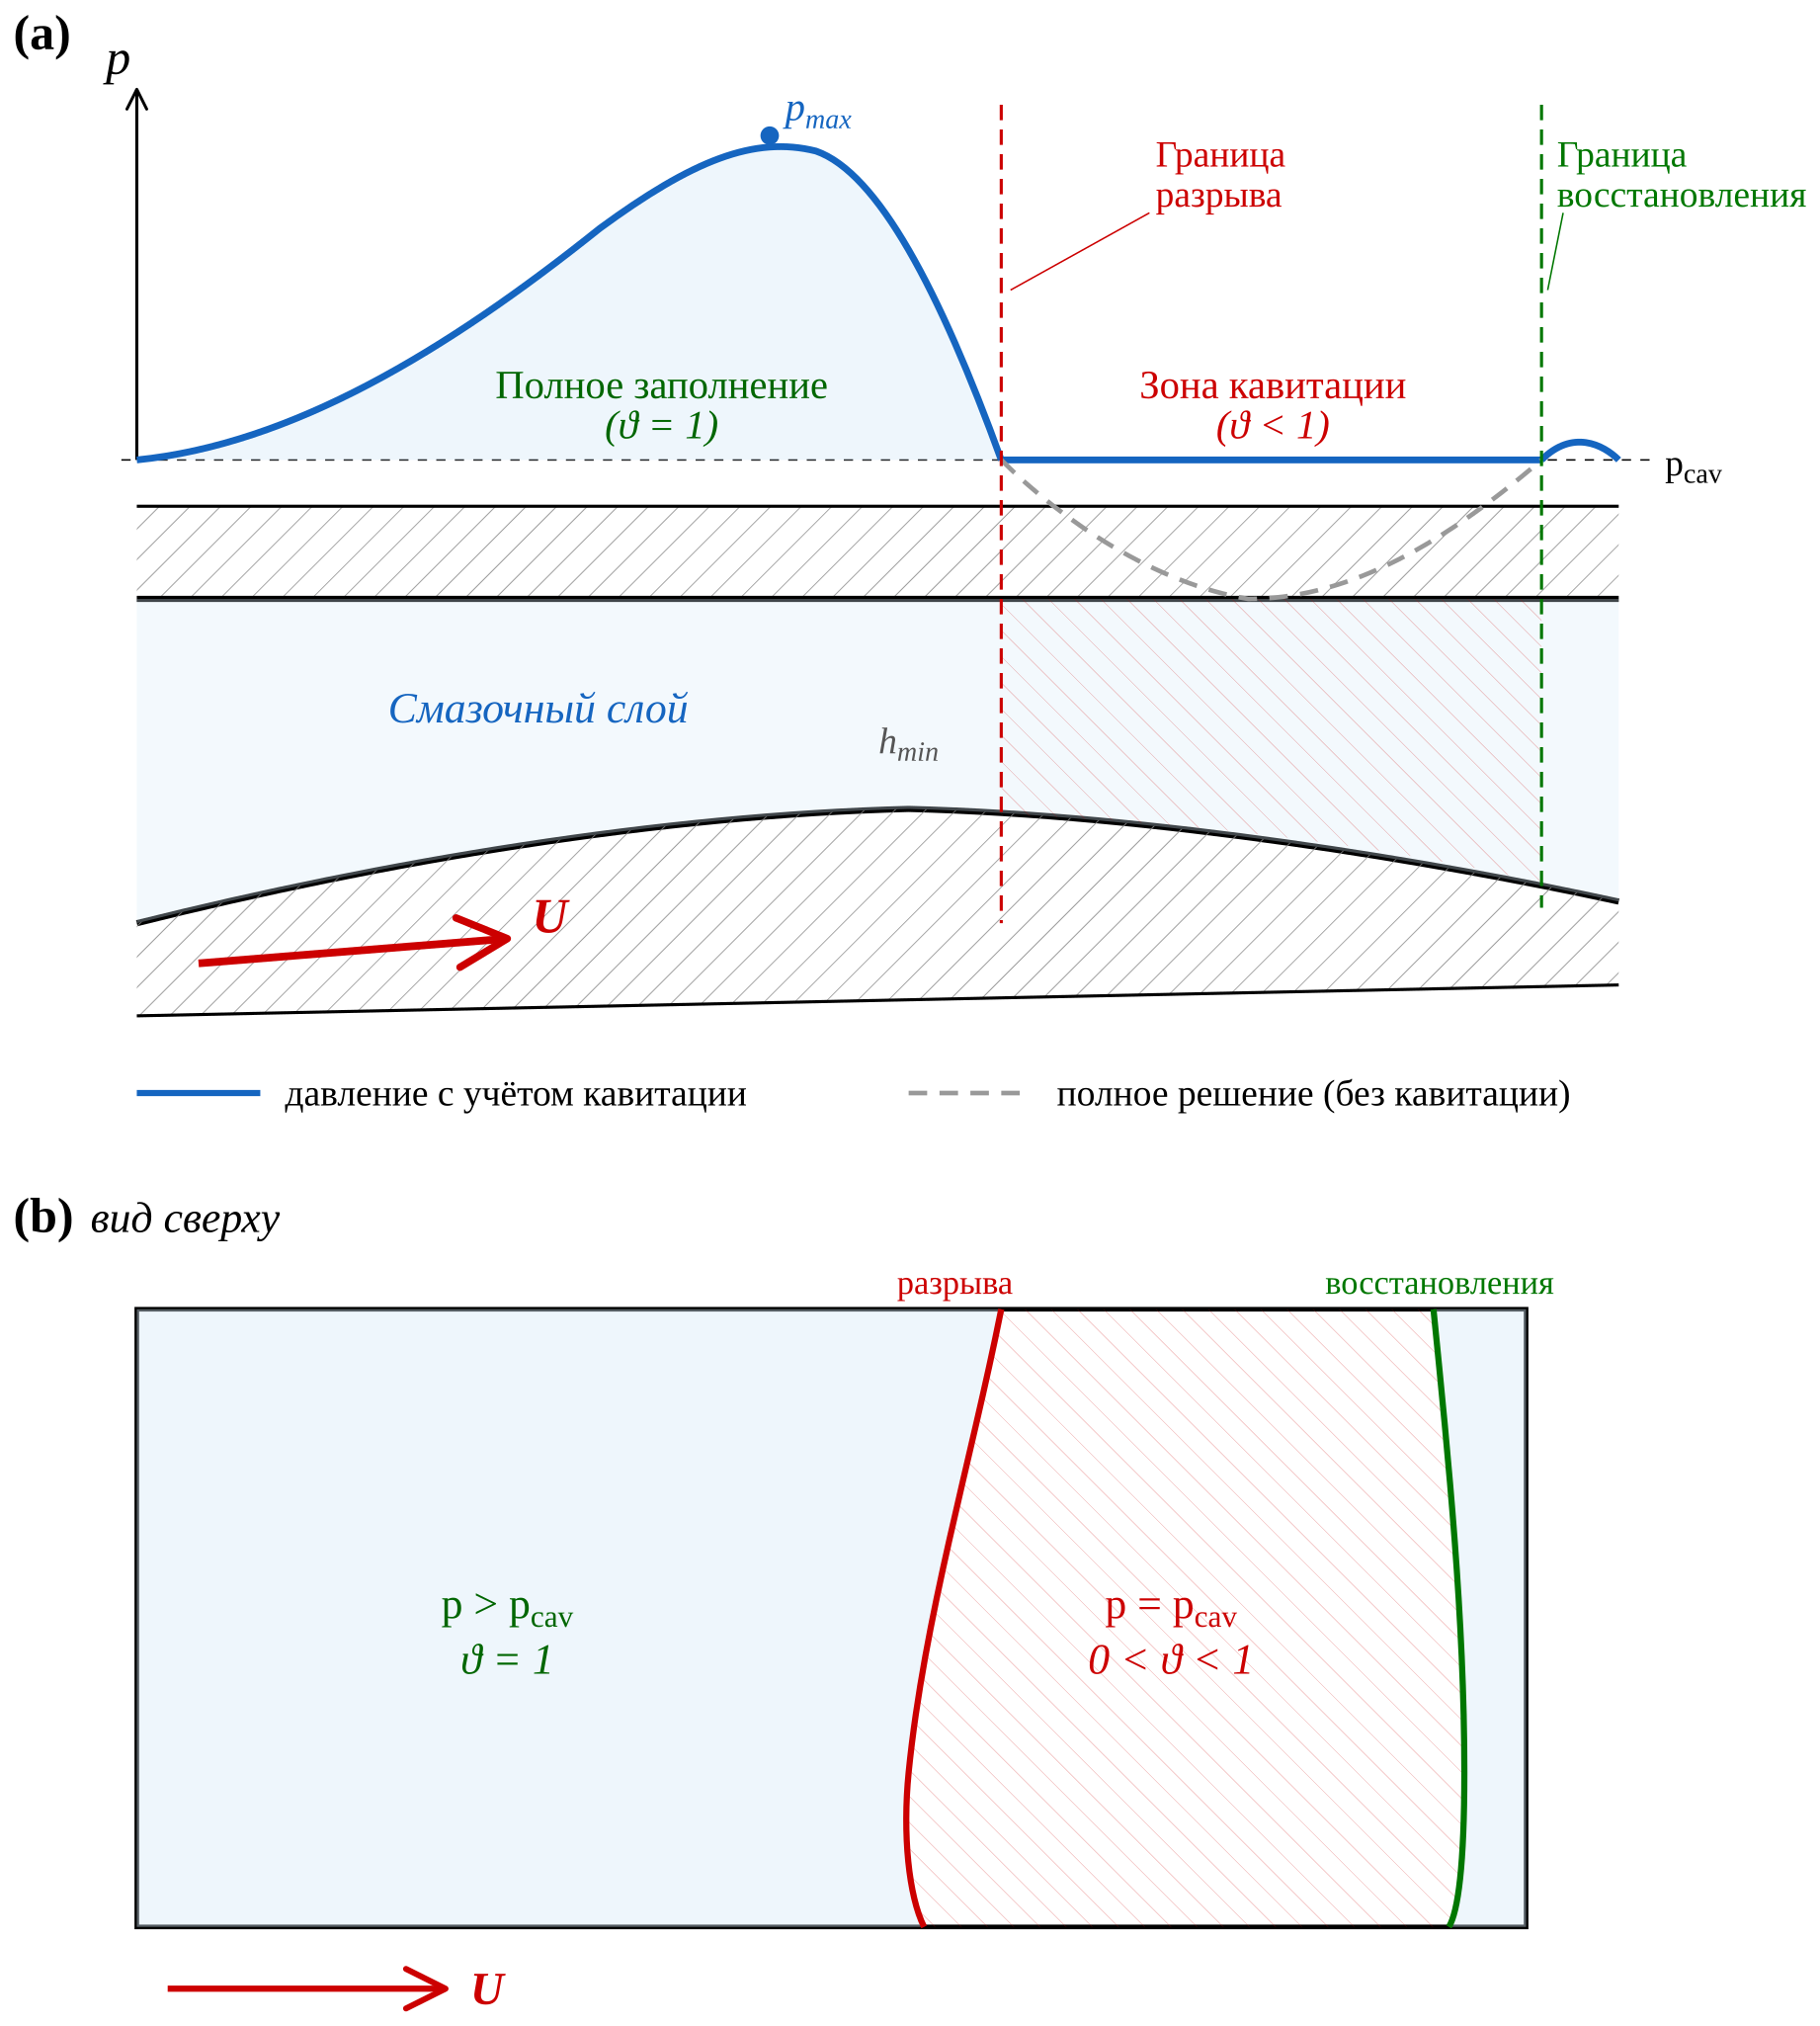
\includegraphics[width=\textwidth,height=0.9\textheight,keepaspectratio]{figures/ch02/fig_2_18.png}
\caption{Схема кавитации в смазочном слое: продольный разрез~(a)
  и вид сверху~(b)}
\label{fig:cavitation_scheme}
\end{figure}

%% Блок 3: Простой приём — обнуление давления
Наиболее распространённый инженерный подход к устранению нефизичных
отрицательных давлений состоит в замене~$p$ на~$p_{\mathrm{cav}}$
в областях, где решение даёт $p < p_{\mathrm{cav}}$.
Этот приём (условие Гюмбеля, half-Sommerfeld) позволяет получить
приемлемые оценки несущей способности и формы поля давления.
Однако он является неполной физической моделью, поскольку
кавитация -- не просто $p = p_{\mathrm{cav}}$, а ещё и частичное
заполнение зазора.

%% Блок 4: Главный недостаток — нарушение баланса массы
Уравнение Рейнольдса выведено из уравнения неразрывности при
допущении полного заполнения зазора ($\vartheta = 1$, где $\vartheta$ --
степень заполнения).  Типовой удельный расход (объёмный поток) в плёнке имеет вид
\begin{equation}\label{eq:q_film}
  \mathbf{q} = -\frac{h^3}{12\mu}\,\nabla p
    + \frac{h}{2}\,\mathbf{U},
\end{equation}
где $\mathbf{U}$ -- скорость относительного скольжения поверхностей.
Для полностью заполненного зазора ($\vartheta = 1$) выполняется
уравнение неразрывности:
\begin{equation}\label{eq:continuity_film}
  \frac{\partial h}{\partial t} + \nabla \cdot \mathbf{q} = 0.
\end{equation}

Если «отрезать» отрицательные давления, то меняется градиент
давления~$\nabla p$ и, следовательно, поток~$\mathbf{q}$, но при этом
не вводится переменная, описывающая частичное заполнение.  В результате
на границах кавитационной зоны возникают нефизичные источники или стоки
массы.  Эффект особенно заметен при расчётах расхода смазки
и в нестационарных задачах (подвижные микроструктуры, переходные
режимы).  Таким образом, корректная модель должна одновременно
описывать (а)~давление и (б)~степень заполнения в кавитационной
области.

%% Блок 5: Требования к корректной модели кавитации
Сформулируем минимальные требования к модели кавитации:
\begin{enumerate}
  \item $p \geq p_{\mathrm{cav}}$ во всей расчётной области.
  \item В зоне полного заполнения ($\vartheta = 1$) действует
        классическое уравнение Рейнольдса.
  \item В кавитационной зоне ($\vartheta < 1$) давление фиксировано
        $p = p_{\mathrm{cav}}$, а состояние смеси описывается
        дополнительной переменной $\vartheta \in (0,\, 1]$.
  \item Сохранение массы через границу зон (непрерывность нормальной компоненты потока).
\end{enumerate}

%% Блок 5b: Алгоритм Элрода
Первый практический численный алгоритм решения задачи JFO предложен
Elrod и Adams~\cite{elrod1975}: вводится переключающая функция~$g$
($g=1$ в зоне полного заполнения, $g=0$ в зоне кавитации),
позволяющая записать единое уравнение для всей расчётной области
без явного отслеживания границ кавитации.
Алгоритм Элрода получил широкое распространение и лёг в основу
большинства последующих реализаций массосохраняющей кавитации.
В настоящей работе используется альтернативный подход на основе
итераций по активному множеству (подраздел~2.3.3),
обеспечивающий аналогичный результат.

%% Блок 6: Подводка к JFO
Перечисленным требованиям удовлетворяет массосохраняющая постановка
Якобссона--Флоберга--Ольссона (JFO), в которой кавитационная зона
описывается не только условием $p = p_{\mathrm{cav}}$, но и переменной
степенью заполнения~$\vartheta$.  Соответствующие уравнения формулируются
в подразделе~2.3.2~\cite{dhande2018}.

\FloatBarrier
\subsection{Массосохраняющая постановка кавитации (JFO)}

%% Блок 1: Вводный абзац
В подразделе~2.3.1 введены кавитационное давление~$p_{\mathrm{cav}}$
и степень заполнения~$\vartheta \in (0,\,1]$.  Цель настоящего раздела --
записать замкнутую систему уравнений для двух искомых переменных:
давления $p(x_1, x_2, t)$ и степени заполнения
$\vartheta(x_1, x_2, t)$, удовлетворяющую требованиям~1-4,
сформулированным в подразделе~2.3.1.  Толщина зазора
$h(x_1, x_2, t)$ считается заданной (суперпозиция из
подраздела~2.2.1).

%% Блок 2: Модифицированное уравнение неразрывности
В кавитационной зоне зазор заполнен жидкостью лишь частично,
поэтому эффективная толщина жидкого слоя равна~$\vartheta\,h$.
Подстановка этой величины в уравнение неразрывности приводит
к модифицированному уравнению Рейнольдса (уравнение JFO):
\begin{equation}\label{eq:jfo_conservation}
  \frac{\partial (\vartheta\,h)}{\partial t}
  + \nabla \cdot \!\left(
    -\,\frac{h^3}{12\mu}\,\nabla p
    + \frac{\vartheta\,h}{2}\,\mathbf{U}
  \right) = 0.
\end{equation}

Первое слагаемое в дивергенции представляет собой пуазейлевский
(напорный) поток, пропорциональный градиенту давления~$\nabla p$.
Второе слагаемое -- куэттовский (переносной) поток, обусловленный
движением поверхности со скоростью~$\mathbf{U}$.  При $\vartheta = 1$
уравнение~\eqref{eq:jfo_conservation} сводится к классическому
уравнению Рейнольдса.  Здесь операторы $\nabla$ и $\nabla\!\cdot$
понимаются в поверхностных координатах, соответствующих выбранной
постановке (подраздел~2.1.6).  Множитель~$\vartheta$ входит в член
накопления и в куэттовский поток.  В кавитационной зоне
$p = p_{\mathrm{cav}}$, поэтому $\nabla p = 0$ и напорный поток
отсутствует автоматически.

Принципиальное отличие постановки JFO от упрощённых моделей кавитации состоит в~следующем. В~модели Гюмбеля отрицательные давления просто обнуляются: $p := \max(p,\, p_{\mathrm{cav}})$ без какого-либо уравнения для кавитационной зоны. Это нарушает баланс масс: куэттовский поток в~зону кавитации не~компенсируется потоком из~неё, и~расход жидкости через замкнутый контур оказывается ненулевым. Следствием является систематическое завышение несущей способности по сравнению с~более точными расчётами, что подтверждается экспериментально: при высоких числах Зоммерфельда отклонение может достигать десятков процентов.

В~постановке JFO вместо простого обнуления давления вводится степень заполнения~$\vartheta$, которая описывает долю объёма зазора, занятую жидкостью. В~зоне полного заполнения $\vartheta = 1$ и~уравнение~\eqref{eq:jfo_conservation} совпадает с~классическим уравнением Рейнольдса. В~кавитационной зоне $p = p_{\mathrm{cav}}$ и~$\vartheta < 1$: жидкость и~газовые пузырьки сосуществуют в~зазоре, причём их~относительные доли изменяются так, чтобы выполнялся баланс масс. Именно введение~$\vartheta$ позволяет разрешить противоречие: давление не~опускается ниже~$p_{\mathrm{cav}}$, а~массовый баланс при~этом сохраняется.

Принципиальное отличие постановки JFO от упрощённых моделей кавитации состоит в~следующем. В~модели Гюмбеля отрицательные давления просто обнуляются: $p := \max(p,\, p_{\mathrm{cav}})$ без какого-либо уравнения для кавитационной зоны. Это нарушает баланс масс: куэттовский поток в~зону кавитации не~компенсируется потоком из~неё, и~расход жидкости через замкнутый контур оказывается ненулевым. Следствием является систематическое завышение несущей способности по сравнению с~более точными расчётами, что подтверждается экспериментально: при высоких числах Зоммерфельда отклонение может достигать десятков процентов.

В~постановке JFO вместо простого обнуления давления вводится степень заполнения~$\vartheta$, которая описывает долю объёма зазора, занятую жидкостью. В~зоне полного заполнения $\vartheta = 1$ и~уравнение~\eqref{eq:jfo_conservation} совпадает с~классическим уравнением Рейнольдса. В~кавитационной зоне $p = p_{\mathrm{cav}}$ и~$\vartheta < 1$: жидкость и~газовые пузырьки сосуществуют в~зазоре, причём их~относительные доли изменяются так, чтобы выполнялся баланс масс. Именно введение~$\vartheta$ позволяет разрешить противоречие: давление не~опускается ниже~$p_{\mathrm{cav}}$, а~массовый баланс при~этом сохраняется.

%% Блок 3: Условия комплементарности
Разделение расчётной области на зону полного заполнения и зону
кавитации определяется условиями комплементарности:
\begin{equation}\label{eq:jfo_complementarity}
  \begin{aligned}
    &p - p_{\mathrm{cav}} \geq 0, \\
    &0 \leq \vartheta \leq 1, \\
    &(p - p_{\mathrm{cav}})\,(1 - \vartheta) = 0.
  \end{aligned}
\end{equation}

Из этих условий следует: либо $p > p_{\mathrm{cav}}$ и тогда
$\vartheta = 1$ (полное заполнение), либо $\vartheta < 1$ и тогда
$p = p_{\mathrm{cav}}$ (кавитация).  Промежуточные состояния
($p > p_{\mathrm{cav}}$ и одновременно $\vartheta < 1$) исключены.
Вместе с уравнением~\eqref{eq:jfo_conservation}
условия~\eqref{eq:jfo_complementarity} образуют замкнутую задачу
для двух неизвестных~$p$ и~$\vartheta$.

Задача~\eqref{eq:jfo_conservation}--\eqref{eq:jfo_complementarity} относится к~классу задач со~свободными границами. Граница разрыва плёнки~-- линия, на~которой $\vartheta$ убывает от~1 до~значения меньше единицы~-- и~граница восстановления плёнки~-- линия, на~которой $\vartheta$ возвращается к~единице~-- не~фиксируются заранее, а~определяются в~ходе решения как часть ответа. Именно эта особенность делает задачу нелинейной даже при линейном уравнении~\eqref{eq:jfo_conservation}: нелинейность сосредоточена в~условиях комплементарности~\eqref{eq:jfo_complementarity}, которые определяют разбиение расчётной области.

Для гладкой поверхности кавитационная зона, как правило, одна и~связна: плёнка разрывается в~расходящемся клине и~восстанавливается на~входе в~следующий период. При~текстурированной поверхности картина принципиально меняется: каждая лунка формирует собственную локальную кавитационную зону в~своей задней части. В~результате расчётная область содержит множество небольших, пространственно разрозненных кавитационных участков. Для~такого решения обеспечение баланса масс становится критически важным: простое обнуление давления приводит к~тому, что каждая лунка <<теряет>> часть массы, и~суммарная ошибка пропорциональна числу лунок~-- она может достигать значимых величин при~высокой плотности текстуры.

Именно поэтому постановка JFO представляет особую ценность при~анализе подшипников с~детерминированными микроструктурами. При~большом числе лунок (порядка~100 и~более на~расчётную область) ошибка, накапливаемая при~использовании упрощённой кавитации, может искажать как~интегральные характеристики (несущую способность, момент трения), так и~пространственное распределение давления. Массосохраняющая постановка лишена этого недостатка по~построению.

Задача~\eqref{eq:jfo_conservation}--\eqref{eq:jfo_complementarity} относится к~классу задач со~свободными границами. Граница разрыва плёнки~-- линия, на~которой $\vartheta$ убывает от~1 до~значения меньше единицы~-- и~граница восстановления плёнки~-- линия, на~которой $\vartheta$ возвращается к~единице~-- не~фиксируются заранее, а~определяются в~ходе решения как часть ответа. Именно эта особенность делает задачу нелинейной даже при линейном уравнении~\eqref{eq:jfo_conservation}: нелинейность сосредоточена в~условиях комплементарности~\eqref{eq:jfo_complementarity}, которые определяют разбиение расчётной области.

Для гладкой поверхности кавитационная зона, как правило, одна и~связна: плёнка разрывается в~расходящемся клине и~восстанавливается на~входе в~следующий период. При~текстурированной поверхности картина принципиально меняется: каждая лунка формирует собственную локальную кавитационную зону в~своей задней части. В~результате расчётная область содержит множество небольших, пространственно разрозненных кавитационных участков. Для~такого решения обеспечение баланса масс становится критически важным: простое обнуление давления приводит к~тому, что каждая лунка <<теряет>> часть массы, и~суммарная ошибка пропорциональна числу лунок~-- она может достигать значимых величин при~высокой плотности текстуры.

Именно поэтому постановка JFO представляет особую ценность при~анализе подшипников с~детерминированными микроструктурами. При~большом числе лунок (порядка~100 и~более на~расчётную область) ошибка, накапливаемая при~использовании упрощённой кавитации, может искажать как~интегральные характеристики (несущую способность, момент трения), так и~пространственное распределение давления. Массосохраняющая постановка лишена этого недостатка по~построению.

%% Рисунок
\begin{figure}[!ht]
\centering
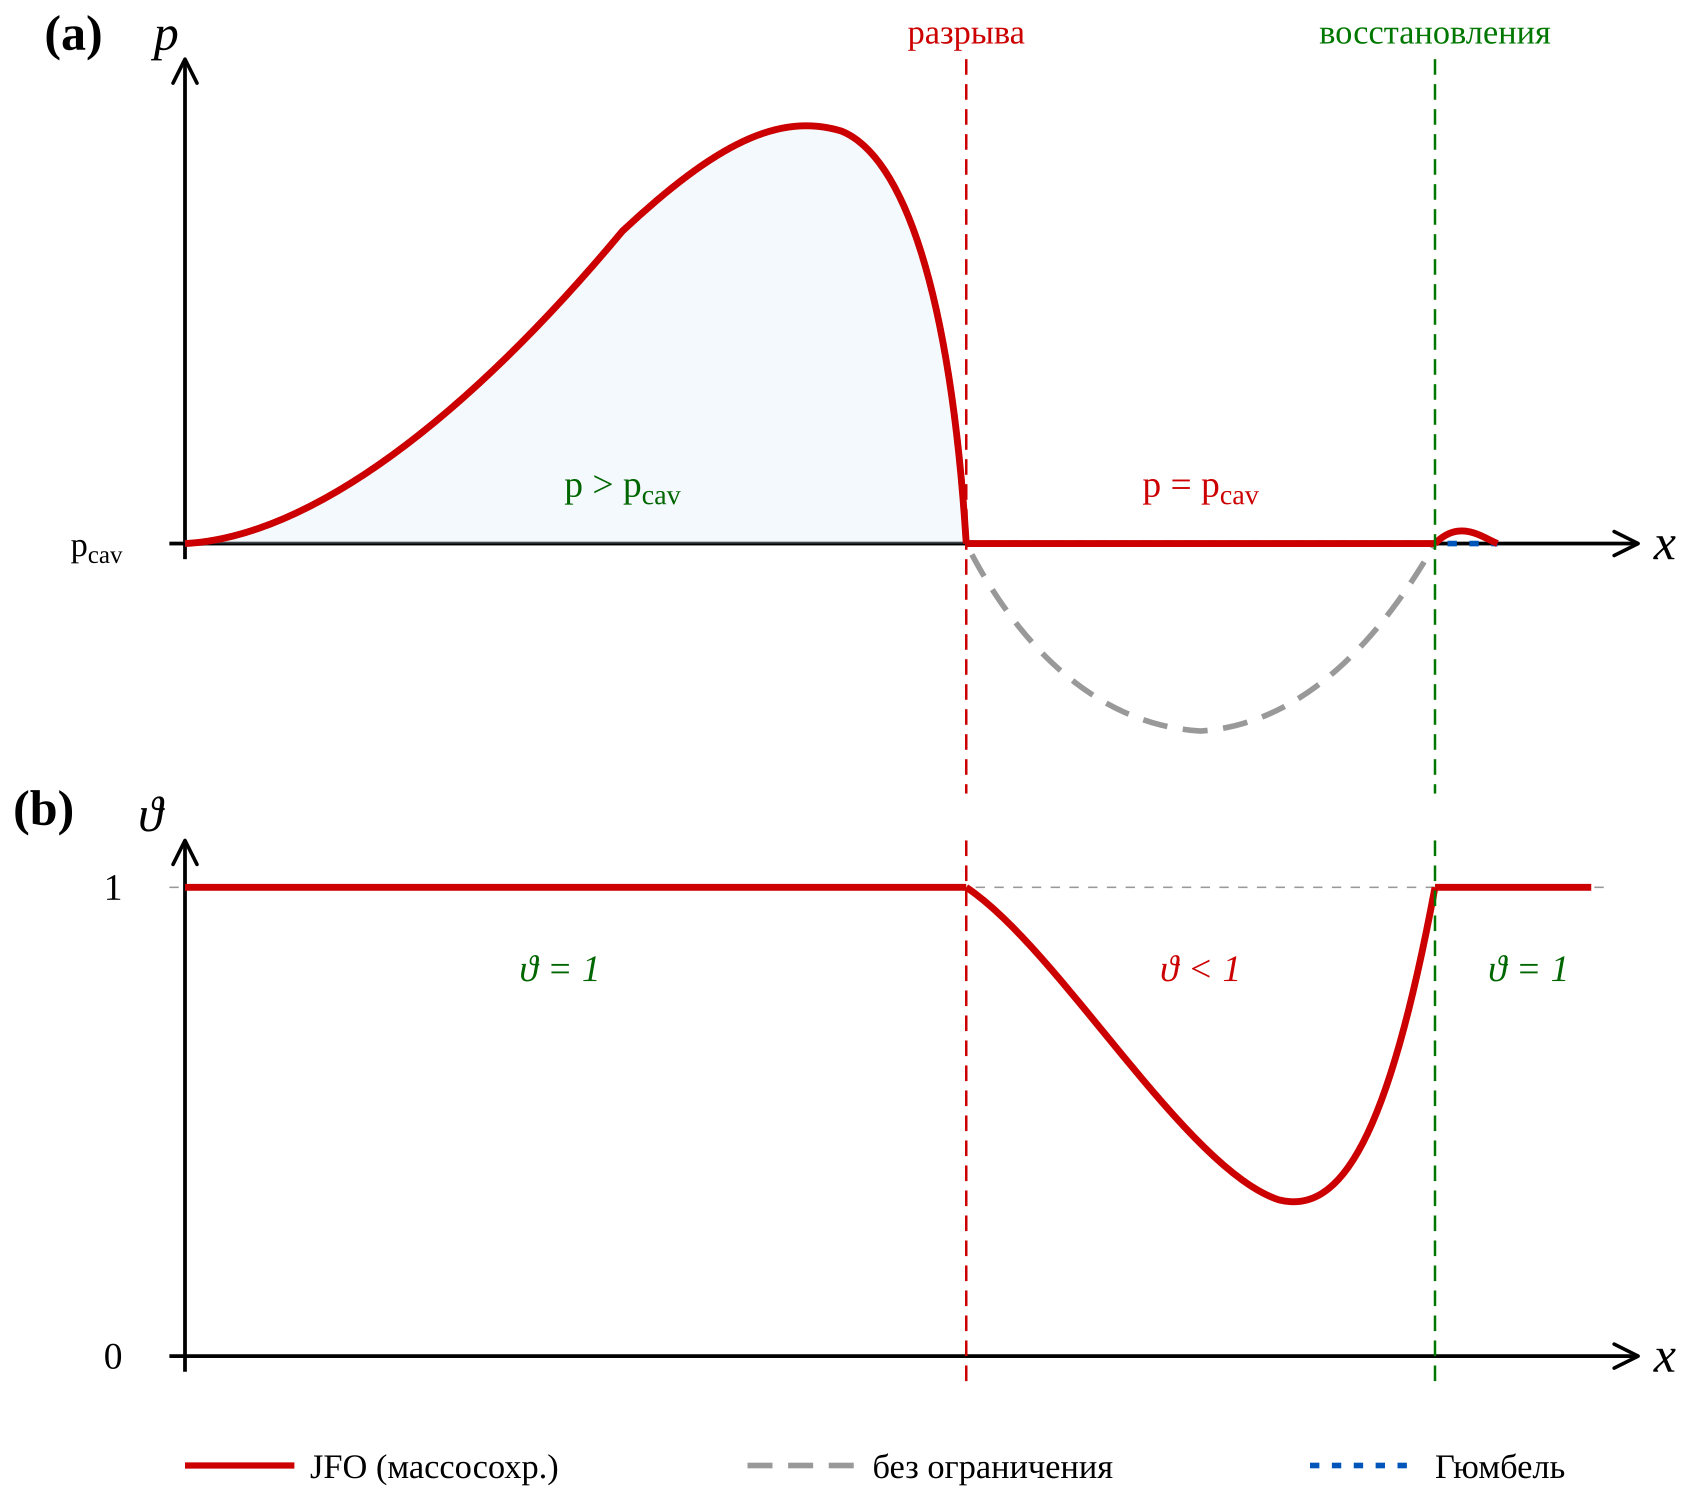
\includegraphics[width=\textwidth,height=0.9\textheight,keepaspectratio]{figures/ch02/fig_2_19.png}
\caption{Сравнение моделей кавитации: обнуление давления (Гюмбель)
  и массосохраняющая постановка (JFO)}
\label{fig:jfo_1d_profile}
\end{figure}

%% Блок 4: Граничные условия
Граничные условия для давления задаются так же, как в
подразделах~2.1.2-2.1.4 (периодичность, заданное давление на входе
и~выходе).  На границах подачи смазки полагают $\vartheta = 1$
(полное заполнение).  По периодическим направлениям~$\vartheta$
подчиняется тем же условиям периодичности, что и~$p$.

%% Блок 5: Подводка к численной реализации
Задача~\eqref{eq:jfo_conservation}-\eqref{eq:jfo_complementarity}
является нелинейной задачей с неравенствами (комплементарность).
На практике её решают итерационно: на каждой итерации определяется
активное множество кавитации и полного заполнения, после чего
обновляются $p$ и $\vartheta$ при выполнении условий комплементарности.
Сравнение моделей кавитации (обнуление давления и JFO) на одномерном профиле давления иллюстрирует рис.~\ref{fig:jfo_1d_profile}. Численная схема дискретизации и алгоритм итерационного решения
приводятся в подразделе~2.3.3~\cite{elrod1975}.

\FloatBarrier
\subsection{Дискретизация уравнений JFO}

%% Блок 1: Вводный абзац
Задача~\eqref{eq:jfo_conservation}-\eqref{eq:jfo_complementarity}
является нелинейной комплементарной задачей: одновременно определяются
давление~$p$ и степень заполнения~$\vartheta$ при выполнении
неравенств.  Решение выполняется итерационно по стратегии активного
множества (active-set): на каждой итерации обновляется разбиение
области на зону полного заполнения и зону кавитации.  В настоящем
подразделе приводится общая схема алгоритма; детали дискретизации,
аппроксимации потоков и выбора солвера описаны в главе~3.

%% Блок 2: Сетка
Расчётная область покрывается равномерной сеткой:
\begin{equation}\label{eq:jfo_grid}
  \begin{aligned}
    &x_{1,i} = x_{1,s} + i\,\Delta x_1, \quad i = 0, \ldots, N_1 - 1, \\
    &x_{2,j} = x_{2,s} + j\,\Delta x_2, \quad j = 0, \ldots, N_2 - 1.
  \end{aligned}
\end{equation}

По периодическим направлениям применяются соответствующие условия
замыкания.  Операторы $\nabla$, $\nabla\!\cdot$ дискретизуются
в поверхностных координатах (подраздел~2.1.6); конкретные разностные
аппроксимации приведены в главе~3.

%% Блок 3: Консервативная дискретизация
Уравнение~\eqref{eq:jfo_conservation} записывается в дискретной
консервативной форме:
\begin{equation}\label{eq:jfo_discrete}
  \frac{(\vartheta h)_{i,j}^{n+1} - (\vartheta h)_{i,j}^{n}}{\Delta t}
  + \frac{F_{i+\frac{1}{2},j} - F_{i-\frac{1}{2},j}}{\Delta x_1}
  + \frac{G_{i,j+\frac{1}{2}} - G_{i,j-\frac{1}{2}}}{\Delta x_2}
  = 0,
\end{equation}
где $F$ и $G$ -- дискретные потоки по направлениям $x_1$ и $x_2$,
соответствующие напорному и переносному слагаемым
в~\eqref{eq:jfo_conservation}.  Потоки аппроксимируются так, чтобы
обеспечить консервативность (сохранение массы на дискретном уровне);
конкретный способ аппроксимации описан в главе~3.  В стационарной
постановке первый член в~\eqref{eq:jfo_discrete} опускается.

%% Блок 4: Идея active-set
На каждой итерации расчётная область разбивается на два множества:
\begin{itemize}
  \item зона полного заполнения: $p_{i,j} > p_{\mathrm{cav}}$,
    при этом $\vartheta_{i,j} = 1$; в этих узлах решается дискретная
    задача для давления~$p$ (уравнение Рейнольдса как частный случай
    при $\vartheta = 1$);
  \item зона кавитации (после проекции): $p_{i,j} = p_{\mathrm{cav}}$,
    при этом $0 \leq \vartheta_{i,j} < 1$; значение~$\vartheta$
    обновляется из дискретного уравнения
    сохранения~\eqref{eq:jfo_discrete}.
\end{itemize}
Переключение узлов между множествами продолжается до стабилизации
активного множества.

%% Блок 5: Псевдокод алгоритма
\begin{enumerate}
  \item Инициализация: $p^{(0)}_{i,j} = p_{\mathrm{cav}}$,
        $\vartheta^{(0)}_{i,j} = 1$.
  \item Цикл по $m = 0, 1, 2, \ldots$:
    \begin{enumerate}
      \item[2.1)] решить дискретную задачу для давления~$p$,
            полученную из~\eqref{eq:jfo_conservation}
            при фиксированном~$\vartheta^{(m)}$
            (и известном $(\vartheta h)^n$ в нестационарном случае);
      \item[2.2)] проекция:
            $p_{i,j} := \max(p_{i,j},\; p_{\mathrm{cav}})$;
      \item[2.3)] обновить активное множество: если
            $p_{i,j} > p_{\mathrm{cav}} + \varepsilon$ --
            полное заполнение ($\vartheta_{i,j} = 1$),
            иначе (после проекции
            $p_{i,j} = p_{\mathrm{cav}}$) -- кавитация
            (обновить $\vartheta_{i,j}$
            из~\eqref{eq:jfo_discrete});
      \item[2.4)] отсечка:
            $\vartheta_{i,j} := \min(1,\,\max(0,\,\vartheta_{i,j}))$;
      \item[2.5)] проверка сходимости.
    \end{enumerate}
  \item Выход: $p_{i,j}$, $\vartheta_{i,j}$.
\end{enumerate}
Здесь $\varepsilon$ -- малый численный допуск для устойчивого
определения активного множества.

\textit{Устойчивость и~сходимость алгоритма активного множества.}
Сходимость алгоритма активного множества в~задачах с~комплементарными ограничениями не~гарантирована в~общем случае. Для~задачи JFO, однако, можно указать условия, при~которых итерации сходятся. При~достаточно малом шаге сетки и~гладком поле зазора алгоритм обычно стабилизируется за~10--30 внешних итераций. Ключевым параметром является допуск~$\varepsilon$ в~шаге~2.3: при слишком малом~$\varepsilon$ возникают осцилляции активного множества (узлы на~границе кавитации попеременно переключаются между зонами), при~слишком большом~--- граница размывается и~нарушается точность условий комплементарности. Рекомендуемый диапазон: $\varepsilon$ порядка $10^{-6}$--$10^{-4}$ в~единицах характерного давления.

\textit{Чувствительность к~начальному приближению.}
Начальное приближение $p^{(0)} = p_{\mathrm{cav}}$, $\vartheta^{(0)} = 1$ (полное заполнение) является стандартным и~работоспособным, однако не~оптимальным с~точки зрения скорости сходимости. При~параметрических расчётах, когда вычисляется серия решений при~близких значениях параметра (например, различных эксцентриситетах или~нагрузках), существенного ускорения можно достичь методом тёплого старта: решение предыдущей задачи используется как~начальное приближение для~следующей. При~этом число внешних итераций сокращается в~несколько раз, поскольку активное множество уже близко к~истинному.

\textit{Преимущества консервативной дискретизации.}
Консервативная форма~\eqref{eq:jfo_discrete} обладает рядом важных свойств. Во-первых, она обеспечивает точный баланс масс на~каждой ячейке: суммарный поток через все~грани ячейки равен изменению накопленной массы за~шаг по~времени~--- это свойство выполняется точно, без~погрешности аппроксимации в~балансе. Во-вторых, консервативная схема устойчива к~разрывным полям~$\vartheta$, которые возникают на~границах кавитационных зон. Неконсервативные схемы (например, аппроксимация дивергентного оператора через центральные разности без~консервативных потоков на~гранях) могут давать локальные нарушения баланса масс вблизи границы кавитации, что проявляется в~физически нереалистичных осцилляциях давления и~степени заполнения. Консервативная схема свободна от~этого недостатка и~является предпочтительной при~расчёте подшипников с~множественными кавитационными зонами.

\textit{Устойчивость и~сходимость алгоритма активного множества.}
Сходимость алгоритма активного множества в~задачах с~комплементарными ограничениями не~гарантирована в~общем случае. Для~задачи JFO, однако, можно указать условия, при~которых итерации сходятся. При~достаточно малом шаге сетки и~гладком поле зазора алгоритм обычно стабилизируется за~10--30 внешних итераций. Ключевым параметром является допуск~$\varepsilon$ в~шаге~2.3: при слишком малом~$\varepsilon$ возникают осцилляции активного множества (узлы на~границе кавитации попеременно переключаются между зонами), при~слишком большом~--- граница размывается и~нарушается точность условий комплементарности. Рекомендуемый диапазон: $\varepsilon$ порядка $10^{-6}$--$10^{-4}$ в~единицах характерного давления.

\textit{Чувствительность к~начальному приближению.}
Начальное приближение $p^{(0)} = p_{\mathrm{cav}}$, $\vartheta^{(0)} = 1$ (полное заполнение) является стандартным и~работоспособным, однако не~оптимальным с~точки зрения скорости сходимости. При~параметрических расчётах, когда вычисляется серия решений при~близких значениях параметра (например, различных эксцентриситетах или~нагрузках), существенного ускорения можно достичь методом тёплого старта: решение предыдущей задачи используется как~начальное приближение для~следующей. При~этом число внешних итераций сокращается в~несколько раз, поскольку активное множество уже близко к~истинному.

\textit{Преимущества консервативной дискретизации.}
Консервативная форма~\eqref{eq:jfo_discrete} обладает рядом важных свойств. Во-первых, она обеспечивает точный баланс масс на~каждой ячейке: суммарный поток через все~грани ячейки равен изменению накопленной массы за~шаг по~времени~--- это свойство выполняется точно, без~погрешности аппроксимации в~балансе. Во-вторых, консервативная схема устойчива к~разрывным полям~$\vartheta$, которые возникают на~границах кавитационных зон. Неконсервативные схемы (например, аппроксимация дивергентного оператора через центральные разности без~консервативных потоков на~гранях) могут давать локальные нарушения баланса масс вблизи границы кавитации, что проявляется в~физически нереалистичных осцилляциях давления и~степени заполнения. Консервативная схема свободна от~этого недостатка и~является предпочтительной при~расчёте подшипников с~множественными кавитационными зонами.

%% Блок 6: Критерий сходимости
Итерации завершаются при выполнении условия
\[
  \max_{i,j}|p^{(m+1)}_{i,j} - p^{(m)}_{i,j}| < \varepsilon_p
\]
и стабилизации активного множества (ни один узел не переключился
между зонами).  При необходимости дополнительно контролируется
\[
  \max_{i,j}|\vartheta^{(m+1)}_{i,j} - \vartheta^{(m)}_{i,j}|
  < \varepsilon_\vartheta.
\]
Общая логика описанного алгоритма представлена
на рисунке~\ref{fig:jfo_algorithm}.

%% Рисунок: блок-схема алгоритма
\begin{figure}[!ht]
\centering
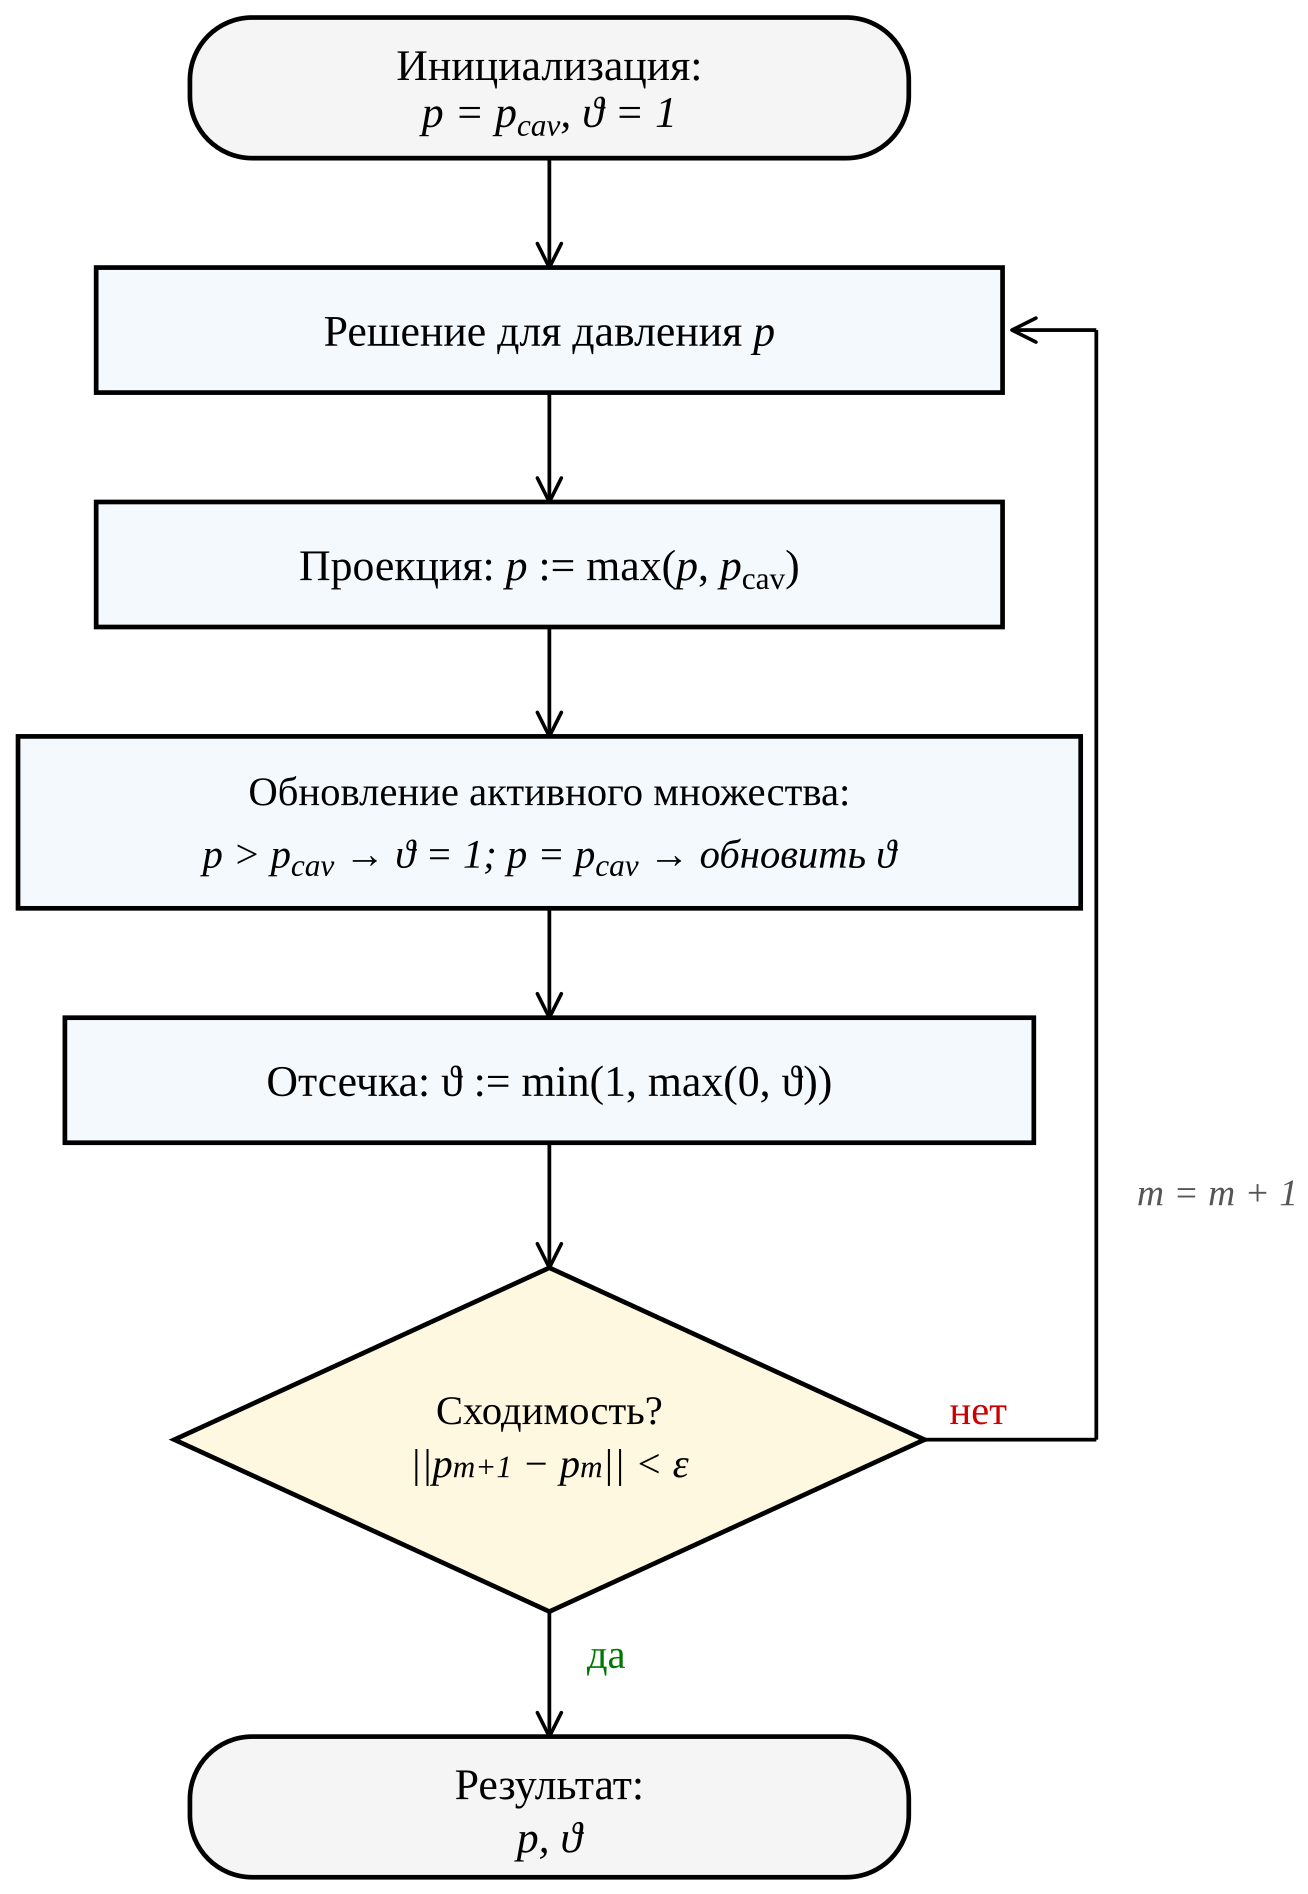
\includegraphics[width=\textwidth,height=0.9\textheight,keepaspectratio]{figures/ch02/fig_2_20.png}
\caption{Блок-схема итерационного алгоритма решения задачи JFO}
\label{fig:jfo_algorithm}
\end{figure}

%% Блок 8: Завершающий абзац
Описанная схема при консервативной аппроксимации потоков обеспечивает
массосохраняющее решение задачи кавитации~\cite{elrod1975,meng2017}
и применяется далее ко всем рассматриваемым постановкам (упорный,
радиальный и возвратно-поступательный подшипники).  Подробности
реализации, включая аппроксимацию потоков на гранях ячеек, выбор
солвера и диагностику баланса массы, приведены в главе~3.


% \FloatBarrier
% \FloatBarrier
\section*{Выводы по главе 2}
\phantomsection\addcontentsline{toc}{section}{Выводы по главе 2}

В главе~2 сформулирована единая математическая основа для численного
моделирования смазочного слоя в подшипниках скольжения как для гладкой,
так и для детерминированно микроструктурированной рабочей поверхности.

\begin{enumerate}[wide, labelindent=\parindent, nosep]
  \item Для трёх типовых постановок (упорной, радиальной
    и возвратно-поступательной) введены согласованные поверхностные
    координаты, масштабы безразмеризации и унифицированная форма
    уравнения Рейнольдса, что обеспечивает сопоставимость результатов
    и возможность переноса алгоритмов между постановками.
  \item Сформулирована параметрическая модель детерминированного
    микрорельефа в виде добавки к базовой функции зазора:
    $h = h_{\mathrm{base}} + \Delta h$, где $\Delta h$ задаётся суммой
    вкладов локализованных элементов.  Введены основные геометрические
    параметры элемента (глубина~$h_p$, полуоси~$a$, $b$,
    ориентация~$\alpha$, параметр плоского дна~$\rho_0$,
    длина канавок~$\ell$).
  \item Систематизированы типы геометрии микроструктур
    (эллипсоидальная, параболическая, коническая, косинусная, smoothstep,
    с плоским дном -- для эллиптических элементов; поперечный
    и продольный профили -- для канавок).
    Описаны типы раскладки элементов на поверхности (прямоугольная,
    шахматная, гексагональная, спиральная по принципу филлотаксиса,
    а также раскладка канавок) и сформулировано правило включения
    элементов в область текстурирования.
  \item Введён компактный набор безразмерных параметров микрорельефа
    ($H_p$, $A^{*}$, $B^{*}$, $\kappa$, $P_1^{*}$, $P_2^{*}$, $\phi$,
    $\rho_0$, $\ell^{*}$), позволяющий проводить параметрические
    исследования и сравнивать различные конфигурации при одинаковых
    безразмерных параметрах.
  \item Рассмотрена физическая природа кавитации и показаны ограничения
    инженерного подхода отсечения давления снизу (условие Гюмбеля),
    связанные с нарушением баланса массы.  Для корректного учёта разрыва
    плёнки сформулирована массосохраняющая постановка кавитации (JFO),
    включающая уравнение
    сохранения для~$\vartheta h$ и условия комплементарности
    для~$p$ и~$\vartheta$.
  \item Описана связь постановки JFO с численной реализацией:
    дискретизация в консервативной форме и итерационное решение методом
    активного множества.  Подробности дискретизации потоков, выбора
    решателя и проверки массобаланса вынесены в главу~3.
\end{enumerate}

Сформулированные модели, параметризация микрорельефа и массосохраняющая
модель кавитации (JFO) образуют основу для реализации расчётного алгоритма
и проведения вычислительных экспериментов, представленных в последующих
главах.


\FloatBarrier
\section*{Контрольные вопросы}
\phantomsection\addcontentsline{toc}{section}{Контрольные вопросы}

\begin{enumerate}
\item Из~каких уравнений выводится уравнение Рейнольдса?
\item Какие допущения используются при~выводе уравнения Рейнольдса?
\item Как~записывается уравнение Рейнольдса для~плоскопараллельной задачи (упорный подшипник)?
\item В~чём отличие постановки задачи для~радиального и~упорного подшипников?
\item Как~учитывается геометрия микрорельефа в~функции зазора?
\item Какие схемы расположения элементов микрорельефа существуют (кольцевое, шахматное, филлотаксис)?
\item Что~такое безразмеризация и~зачем она~применяется?
\item Что~такое модель JFO и~какую проблему она~решает?
\item Как~формулируются граничные условия при~кавитации?
\item Какие функционалы используются для~оценки характеристик подшипника?
\item Что~такое условия комплементарности в~постановке JFO?
\item В~чём состоит конкуренция двух гидродинамических эффектов при~текстурировании поверхности?
\end{enumerate}
